\PassOptionsToPackage{unicode=true}{hyperref} % options for packages loaded elsewhere
\PassOptionsToPackage{hyphens}{url}
%
\documentclass[]{book}
\usepackage{lmodern}
\usepackage{amssymb,amsmath}
\usepackage{ifxetex,ifluatex}
\usepackage{fixltx2e} % provides \textsubscript
\ifnum 0\ifxetex 1\fi\ifluatex 1\fi=0 % if pdftex
  \usepackage[T1]{fontenc}
  \usepackage[utf8]{inputenc}
  \usepackage{textcomp} % provides euro and other symbols
\else % if luatex or xelatex
  \usepackage{unicode-math}
  \defaultfontfeatures{Ligatures=TeX,Scale=MatchLowercase}
\fi
% use upquote if available, for straight quotes in verbatim environments
\IfFileExists{upquote.sty}{\usepackage{upquote}}{}
% use microtype if available
\IfFileExists{microtype.sty}{%
\usepackage[]{microtype}
\UseMicrotypeSet[protrusion]{basicmath} % disable protrusion for tt fonts
}{}
\IfFileExists{parskip.sty}{%
\usepackage{parskip}
}{% else
\setlength{\parindent}{0pt}
\setlength{\parskip}{6pt plus 2pt minus 1pt}
}
\usepackage{hyperref}
\hypersetup{
            pdftitle={behaviouR: R package and tutorials for online teaching of fundamental concepts in behavior and ecology},
            pdfauthor={Dena J. Clink},
            pdfborder={0 0 0},
            breaklinks=true}
\urlstyle{same}  % don't use monospace font for urls
\usepackage{color}
\usepackage{fancyvrb}
\newcommand{\VerbBar}{|}
\newcommand{\VERB}{\Verb[commandchars=\\\{\}]}
\DefineVerbatimEnvironment{Highlighting}{Verbatim}{commandchars=\\\{\}}
% Add ',fontsize=\small' for more characters per line
\usepackage{framed}
\definecolor{shadecolor}{RGB}{248,248,248}
\newenvironment{Shaded}{\begin{snugshade}}{\end{snugshade}}
\newcommand{\AlertTok}[1]{\textcolor[rgb]{0.94,0.16,0.16}{#1}}
\newcommand{\AnnotationTok}[1]{\textcolor[rgb]{0.56,0.35,0.01}{\textbf{\textit{#1}}}}
\newcommand{\AttributeTok}[1]{\textcolor[rgb]{0.77,0.63,0.00}{#1}}
\newcommand{\BaseNTok}[1]{\textcolor[rgb]{0.00,0.00,0.81}{#1}}
\newcommand{\BuiltInTok}[1]{#1}
\newcommand{\CharTok}[1]{\textcolor[rgb]{0.31,0.60,0.02}{#1}}
\newcommand{\CommentTok}[1]{\textcolor[rgb]{0.56,0.35,0.01}{\textit{#1}}}
\newcommand{\CommentVarTok}[1]{\textcolor[rgb]{0.56,0.35,0.01}{\textbf{\textit{#1}}}}
\newcommand{\ConstantTok}[1]{\textcolor[rgb]{0.00,0.00,0.00}{#1}}
\newcommand{\ControlFlowTok}[1]{\textcolor[rgb]{0.13,0.29,0.53}{\textbf{#1}}}
\newcommand{\DataTypeTok}[1]{\textcolor[rgb]{0.13,0.29,0.53}{#1}}
\newcommand{\DecValTok}[1]{\textcolor[rgb]{0.00,0.00,0.81}{#1}}
\newcommand{\DocumentationTok}[1]{\textcolor[rgb]{0.56,0.35,0.01}{\textbf{\textit{#1}}}}
\newcommand{\ErrorTok}[1]{\textcolor[rgb]{0.64,0.00,0.00}{\textbf{#1}}}
\newcommand{\ExtensionTok}[1]{#1}
\newcommand{\FloatTok}[1]{\textcolor[rgb]{0.00,0.00,0.81}{#1}}
\newcommand{\FunctionTok}[1]{\textcolor[rgb]{0.00,0.00,0.00}{#1}}
\newcommand{\ImportTok}[1]{#1}
\newcommand{\InformationTok}[1]{\textcolor[rgb]{0.56,0.35,0.01}{\textbf{\textit{#1}}}}
\newcommand{\KeywordTok}[1]{\textcolor[rgb]{0.13,0.29,0.53}{\textbf{#1}}}
\newcommand{\NormalTok}[1]{#1}
\newcommand{\OperatorTok}[1]{\textcolor[rgb]{0.81,0.36,0.00}{\textbf{#1}}}
\newcommand{\OtherTok}[1]{\textcolor[rgb]{0.56,0.35,0.01}{#1}}
\newcommand{\PreprocessorTok}[1]{\textcolor[rgb]{0.56,0.35,0.01}{\textit{#1}}}
\newcommand{\RegionMarkerTok}[1]{#1}
\newcommand{\SpecialCharTok}[1]{\textcolor[rgb]{0.00,0.00,0.00}{#1}}
\newcommand{\SpecialStringTok}[1]{\textcolor[rgb]{0.31,0.60,0.02}{#1}}
\newcommand{\StringTok}[1]{\textcolor[rgb]{0.31,0.60,0.02}{#1}}
\newcommand{\VariableTok}[1]{\textcolor[rgb]{0.00,0.00,0.00}{#1}}
\newcommand{\VerbatimStringTok}[1]{\textcolor[rgb]{0.31,0.60,0.02}{#1}}
\newcommand{\WarningTok}[1]{\textcolor[rgb]{0.56,0.35,0.01}{\textbf{\textit{#1}}}}
\usepackage{longtable,booktabs}
% Fix footnotes in tables (requires footnote package)
\IfFileExists{footnote.sty}{\usepackage{footnote}\makesavenoteenv{longtable}}{}
\usepackage{graphicx,grffile}
\makeatletter
\def\maxwidth{\ifdim\Gin@nat@width>\linewidth\linewidth\else\Gin@nat@width\fi}
\def\maxheight{\ifdim\Gin@nat@height>\textheight\textheight\else\Gin@nat@height\fi}
\makeatother
% Scale images if necessary, so that they will not overflow the page
% margins by default, and it is still possible to overwrite the defaults
% using explicit options in \includegraphics[width, height, ...]{}
\setkeys{Gin}{width=\maxwidth,height=\maxheight,keepaspectratio}
\setlength{\emergencystretch}{3em}  % prevent overfull lines
\providecommand{\tightlist}{%
  \setlength{\itemsep}{0pt}\setlength{\parskip}{0pt}}
\setcounter{secnumdepth}{5}
% Redefines (sub)paragraphs to behave more like sections
\ifx\paragraph\undefined\else
\let\oldparagraph\paragraph
\renewcommand{\paragraph}[1]{\oldparagraph{#1}\mbox{}}
\fi
\ifx\subparagraph\undefined\else
\let\oldsubparagraph\subparagraph
\renewcommand{\subparagraph}[1]{\oldsubparagraph{#1}\mbox{}}
\fi

% set default figure placement to htbp
\makeatletter
\def\fps@figure{htbp}
\makeatother

\usepackage{booktabs}
\usepackage{amsthm}
\makeatletter
\def\thm@space@setup{%
  \thm@preskip=8pt plus 2pt minus 4pt
  \thm@postskip=\thm@preskip
}
\makeatother
\usepackage[]{natbib}
\bibliographystyle{plainnat}

\title{behaviouR: R package and tutorials for online teaching of fundamental concepts in behavior and ecology}
\author{Dena J. Clink}
\date{2020-08-25}

\begin{document}
\maketitle

{
\setcounter{tocdepth}{1}
\tableofcontents
}
\hypertarget{welcome}{%
\chapter*{Welcome}\label{welcome}}
\addcontentsline{toc}{chapter}{Welcome}

\begin{center}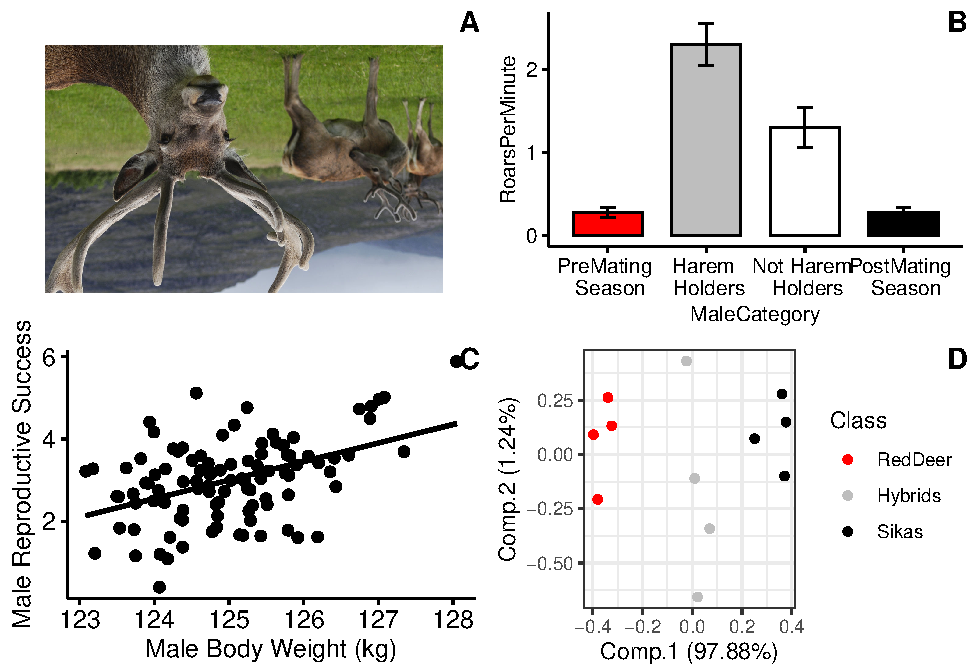
\includegraphics{behaviouR-R-package-tutorials_files/figure-latex/unnamed-chunk-1-1} \end{center}

To get started you should download the package from Github using the following code.

\begin{Shaded}
\begin{Highlighting}[]
\CommentTok{# Install devtools from CRAN}
\KeywordTok{install.packages}\NormalTok{(}\StringTok{"devtools"}\NormalTok{)}

\CommentTok{# Install 'behaviouR' package from Gitub}
\NormalTok{devtools}\OperatorTok{::}\KeywordTok{install_github}\NormalTok{(}\StringTok{"https://github.com/DenaJGibbon/behaviouR"}\NormalTok{)}
\end{Highlighting}
\end{Shaded}

Note: If you have never used R before I highly recommend that you check out the primers here: \url{https://rstudio.cloud/learn/primers}.

You can navigate using the tabs at the left and/or the arrows.

\hypertarget{computer-lab-1.-data-exploration-and-visualization}{%
\chapter*{Computer Lab 1. Data exploration and visualization}\label{computer-lab-1.-data-exploration-and-visualization}}
\addcontentsline{toc}{chapter}{Computer Lab 1. Data exploration and visualization}

\begin{center}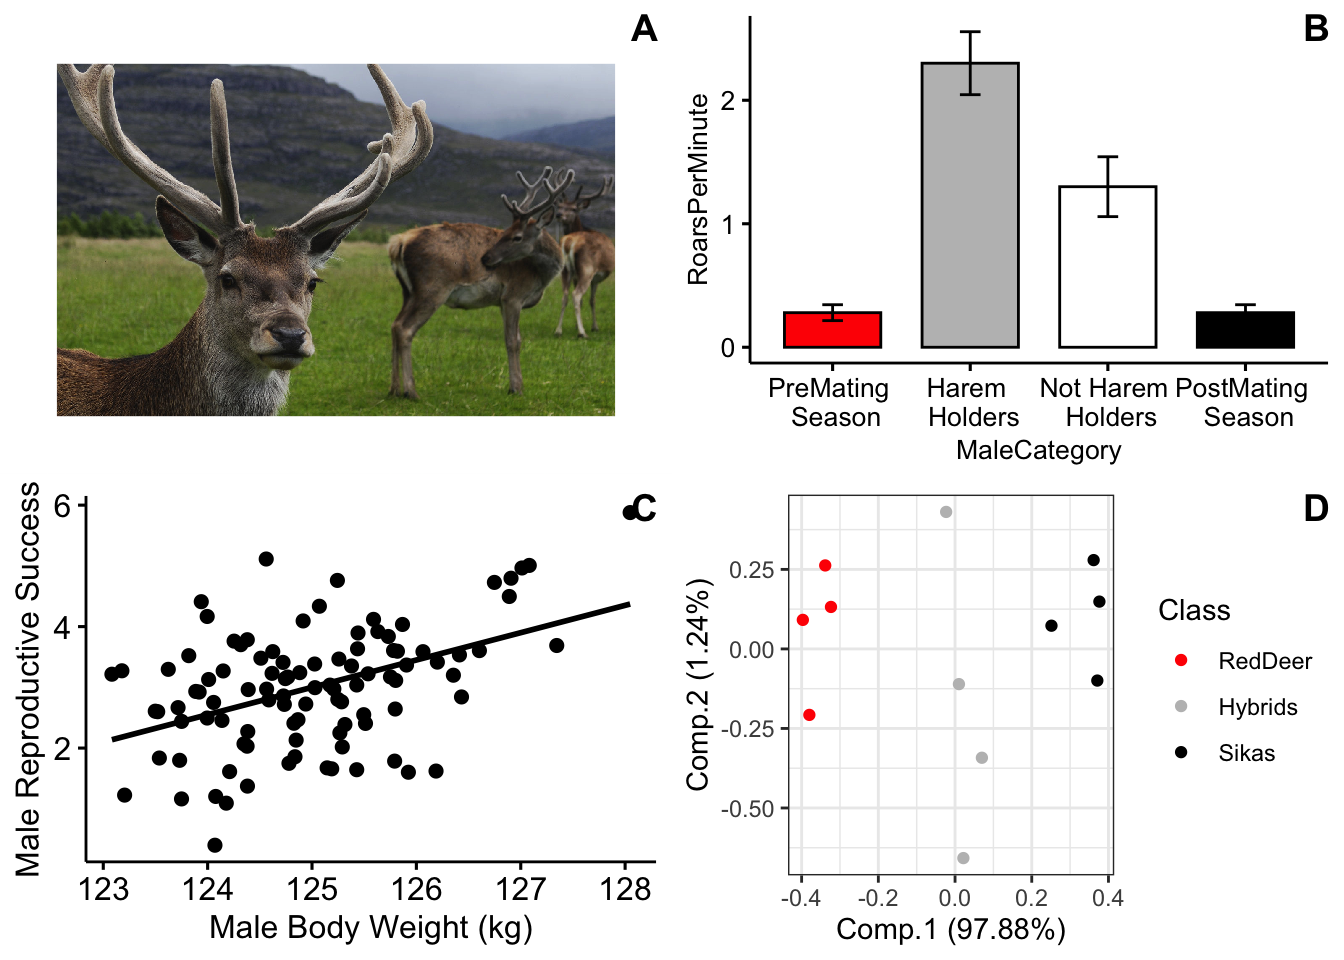
\includegraphics{behaviouR-R-package-tutorials_files/figure-latex/unnamed-chunk-3-1} \end{center}

\emph{Background}\\
Our examples for this lab will focus on roaring behavior in red deer. Red deer on Rum Island, Scotland form harems during the mating season. Harem holding males fight off other males during this time, and many of these males have signs of fighting injuries. Clutton-Brock and colleagues hypothesized that because of the injury associated with fights that red deer males should use honest indicators of each others fighting abilities, and that the main indicator of strength and fighting ability was the male roars.

\emph{Goals of the exercises}\\
The main goal(s) of today's lab are to:\\
1) teach you about different types of data visualization and types of data.\\
2) help you to start to become familiar with using R.\\
3) to get you to think about the ways that scientists analyze data.

\emph{Suggested readings}:\\
Clutton-Brock, Tim H., and Steven D. Albon. ``The roaring of red deer and the evolution of honest advertisement.'' \emph{Behaviour} 69.3-4 (1979): 145-170.

Reby D, McComb K. Anatomical constraints generate honesty: acoustic cues to age and weight in the roars of red deer stags. Animal behaviour. 2003 Mar 1;65(3):519-30.

Long, A. M., N. P. Moore, and T. J. Hayden. ``Vocalizations in red deer (\emph{Cervus elaphus}), sika deer (\emph{Cervus nippon}), and red× sika hybrids.'' Journal of Zoology 244.1 (1998): 123-134.

\emph{Getting started}\\
First we need to load the relevant packages. Packages contain all the functions that are needed for data analysis. The `behaviouR' package loads many other packages that have important functions.

\begin{Shaded}
\begin{Highlighting}[]
\CommentTok{# First we load the relevant packages}
\KeywordTok{library}\NormalTok{(behaviouR)}
\KeywordTok{library}\NormalTok{(ggpubr)}
\KeywordTok{library}\NormalTok{(ggfortify)}
\end{Highlighting}
\end{Shaded}

\hypertarget{part-1.-categorical-data}{%
\section*{Part 1. Categorical data}\label{part-1.-categorical-data}}
\addcontentsline{toc}{section}{Part 1. Categorical data}

Categorical variables represent types of data that can be divided into groups.
Our first example will census a simulated population of red deer to determine the proportion of individuals in different developmental stages.

\begin{Shaded}
\begin{Highlighting}[]
\NormalTok{## Lab 1a. Categorical data}
\CommentTok{# Here we create a simulated population with four categories (Infant, Juvenile, AdultFemale and AdultMale)}
\NormalTok{DeerPopulationDF <-}\StringTok{ }\KeywordTok{data.frame}\NormalTok{(}\DataTypeTok{DevelopmentStage=}\KeywordTok{c}\NormalTok{(}\StringTok{'Infant'}\NormalTok{,}\StringTok{'Juvenile'}\NormalTok{,}\StringTok{'AdultFemale'}\NormalTok{,}\StringTok{'AdultMale'}\NormalTok{),}
                         \DataTypeTok{NumberOfIndividuals=}\KeywordTok{c}\NormalTok{(}\DecValTok{15}\NormalTok{,}\DecValTok{50}\NormalTok{,}\DecValTok{125}\NormalTok{,}\DecValTok{200}\NormalTok{))}

\CommentTok{# We then print the object so that we can see the output}
\NormalTok{DeerPopulationDF}
\end{Highlighting}
\end{Shaded}

\begin{verbatim}
##   DevelopmentStage NumberOfIndividuals
## 1           Infant                  15
## 2         Juvenile                  50
## 3      AdultFemale                 125
## 4        AdultMale                 200
\end{verbatim}

Now we want to plot the data. We will use a simple barplot to start.

Throughout these tutorials we will use functions from the `ggpubr' package for plotting; see \url{https://rpkgs.datanovia.com/ggpubr/} for more details. For more information on the great work the developer is doing see \url{http://www.alboukadel.com/} and \url{http://www.sthda.com/english/}.

\begin{Shaded}
\begin{Highlighting}[]
\CommentTok{# Now we want to plot the data. We will use a simple barplot to start.}
\KeywordTok{ggbarplot}\NormalTok{(DeerPopulationDF, }\DataTypeTok{x=}\StringTok{'DevelopmentStage'}\NormalTok{, }\DataTypeTok{y=}\StringTok{'NumberOfIndividuals'}\NormalTok{)}
\end{Highlighting}
\end{Shaded}

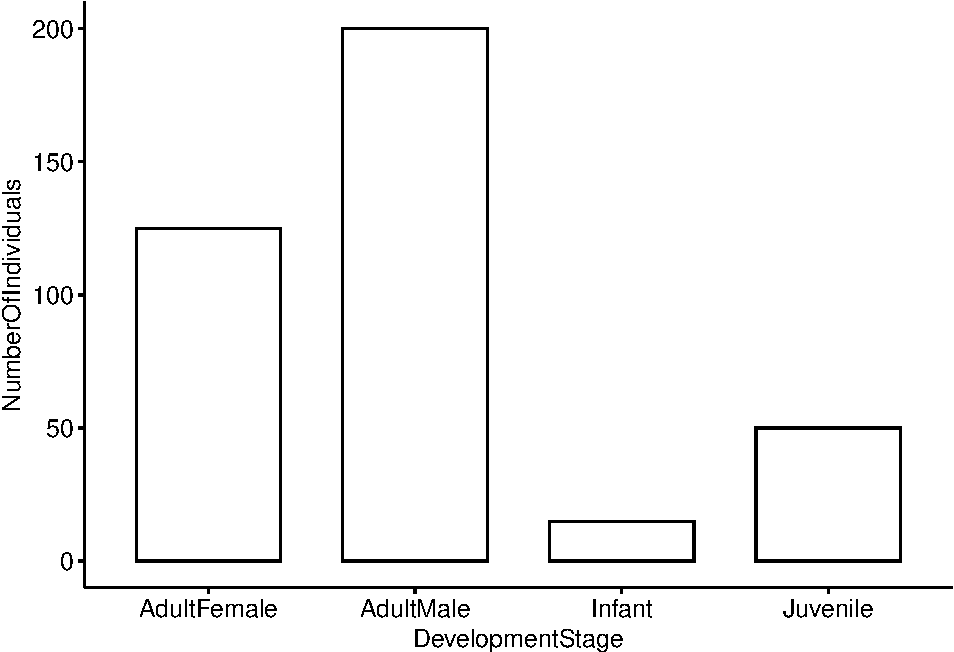
\includegraphics{behaviouR-R-package-tutorials_files/figure-latex/unnamed-chunk-6-1.pdf}

\emph{Please answer the following questions:}\\
Question 1. How would you interpret this figure? Which category has the most individuals, and which has the least?

Question 2a. This is a simulated popuation, but what do you think the ratio of males to females would mean for male-male competition?

Question 2b. Modify the code above so that our simulated deer population has a more even ratio of males to females.

\hypertarget{part-2.-categorical-and-continuous-data}{%
\section*{Part 2. Categorical and continuous data}\label{part-2.-categorical-and-continuous-data}}
\addcontentsline{toc}{section}{Part 2. Categorical and continuous data}

Our second example will investigate roaring rates in deer as a function of status and breeding season. The categories we will use are: pre-mating season, harem holder, not harem holder and post-mating season.Our outcome variable (mean number of roars per minute) is continuous; it represents actual numerical measurements.

We will work with a toy dataset that is based on Figure 2 in Clutton-Brock et al.~1979. For each category we have five observations which represent the average number of calls per minute. For each category we have a total of five observations.

\begin{Shaded}
\begin{Highlighting}[]
\NormalTok{## Lab 1b. Categorical and continuous data}
\CommentTok{# Load the dataset so that we can use it }
\KeywordTok{data}\NormalTok{(}\StringTok{"MaleDeerRoarDF"}\NormalTok{)}

\CommentTok{# We can check the structure of the dataframe by using the command 'head'}
\KeywordTok{head}\NormalTok{(MaleDeerRoarDF)}
\end{Highlighting}
\end{Shaded}

\begin{verbatim}
##      MaleCategory RoarsPerMinute
## 1 PreMatingSeason           0.25
## 2 PreMatingSeason           0.50
## 3 PreMatingSeason           0.25
## 4 PreMatingSeason           0.30
## 5 PreMatingSeason           0.10
## 6    HaremHolders           2.50
\end{verbatim}

Now we will plot the categorical data. First we will use a barplot with error bars representing the standard deviation. See \url{https://www.biologyforlife.com/interpreting-error-bars.html} and \url{https://www.biologyforlife.com/standard-deviation.html} for more information about error bars.

\begin{Shaded}
\begin{Highlighting}[]
\CommentTok{# Now we will plot the categorical data with standard deviations. }
\KeywordTok{ggbarplot}\NormalTok{(MaleDeerRoarDF, }\DataTypeTok{x=}\StringTok{'MaleCategory'}\NormalTok{, }\DataTypeTok{y=}\StringTok{'RoarsPerMinute'}\NormalTok{, }
          \DataTypeTok{add =} \KeywordTok{c}\NormalTok{(}\StringTok{"mean_sd"}\NormalTok{),}\DataTypeTok{xtickslab.rt =} \DecValTok{90}\NormalTok{)}
\end{Highlighting}
\end{Shaded}

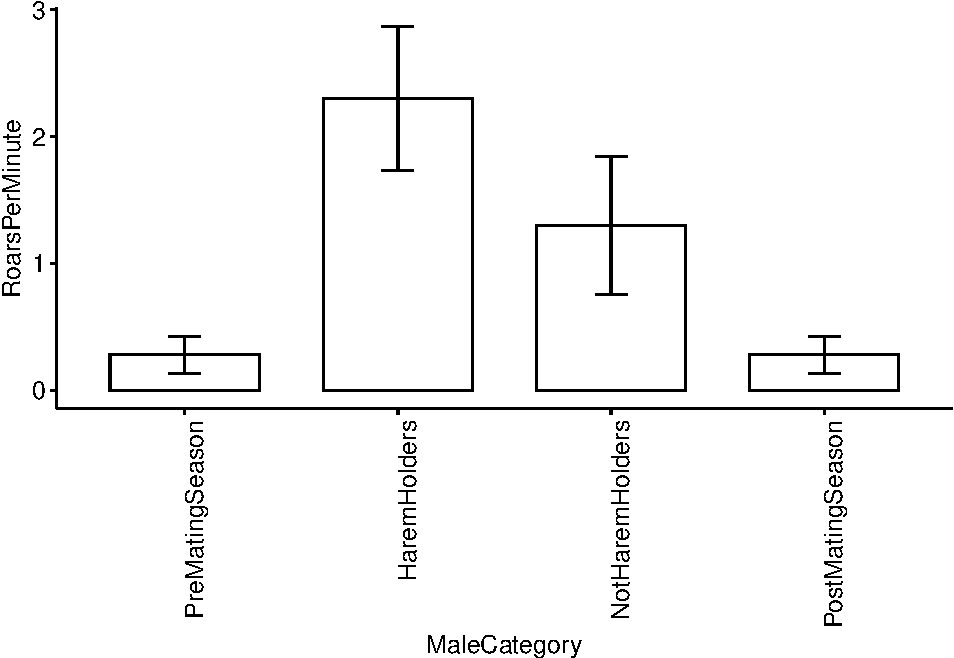
\includegraphics{behaviouR-R-package-tutorials_files/figure-latex/unnamed-chunk-8-1.pdf}

Although it shows us what we need, we can also include some colors in our plot. To do this I added the `fill = 'MaleCategory' argument, which tells R to color the plot based on male categories.

\begin{Shaded}
\begin{Highlighting}[]
\CommentTok{# Now we will plot the categorical data with colors for each category.}
\KeywordTok{ggbarplot}\NormalTok{(MaleDeerRoarDF, }\DataTypeTok{x=}\StringTok{'MaleCategory'}\NormalTok{, }\DataTypeTok{y=}\StringTok{'RoarsPerMinute'}\NormalTok{, }\DataTypeTok{fill =} \StringTok{'MaleCategory'}\NormalTok{,}
          \DataTypeTok{add =} \KeywordTok{c}\NormalTok{(}\StringTok{"mean_sd"}\NormalTok{),}\DataTypeTok{xtickslab.rt =} \DecValTok{90}\NormalTok{)}\OperatorTok{+}\StringTok{ }\KeywordTok{theme}\NormalTok{(}\DataTypeTok{legend.position =} \StringTok{"none"}\NormalTok{)}
\end{Highlighting}
\end{Shaded}

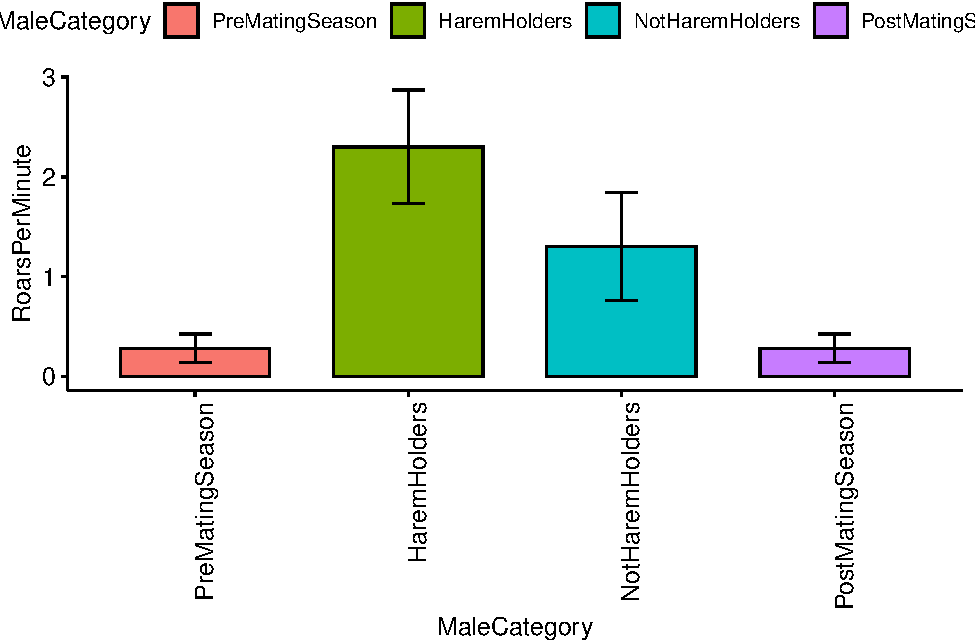
\includegraphics{behaviouR-R-package-tutorials_files/figure-latex/unnamed-chunk-9-1.pdf}

Color for plots is often based on personal preference, below I modified the colors using the `palette' argument.
NOTE: The use of color-blind friendly palettes is becoming increasingly popular among scientists.

\begin{Shaded}
\begin{Highlighting}[]
\CommentTok{# Now we will plot the categorical data with user-specified colors for each category.}
\KeywordTok{ggbarplot}\NormalTok{(MaleDeerRoarDF, }\DataTypeTok{x=}\StringTok{'MaleCategory'}\NormalTok{, }\DataTypeTok{y=}\StringTok{'RoarsPerMinute'}\NormalTok{, }\DataTypeTok{fill =} \StringTok{'MaleCategory'}\NormalTok{,}
          \DataTypeTok{palette =} \KeywordTok{c}\NormalTok{(}\StringTok{'red'}\NormalTok{,}\StringTok{'gray'}\NormalTok{,}\StringTok{'white'}\NormalTok{,}\StringTok{'black'}\NormalTok{),}
          \DataTypeTok{add =} \KeywordTok{c}\NormalTok{(}\StringTok{"mean_se"}\NormalTok{),}\DataTypeTok{xtickslab.rt =} \DecValTok{90}\NormalTok{)}\OperatorTok{+}\StringTok{ }\KeywordTok{theme}\NormalTok{(}\DataTypeTok{legend.position =} \StringTok{"none"}\NormalTok{)}
\end{Highlighting}
\end{Shaded}

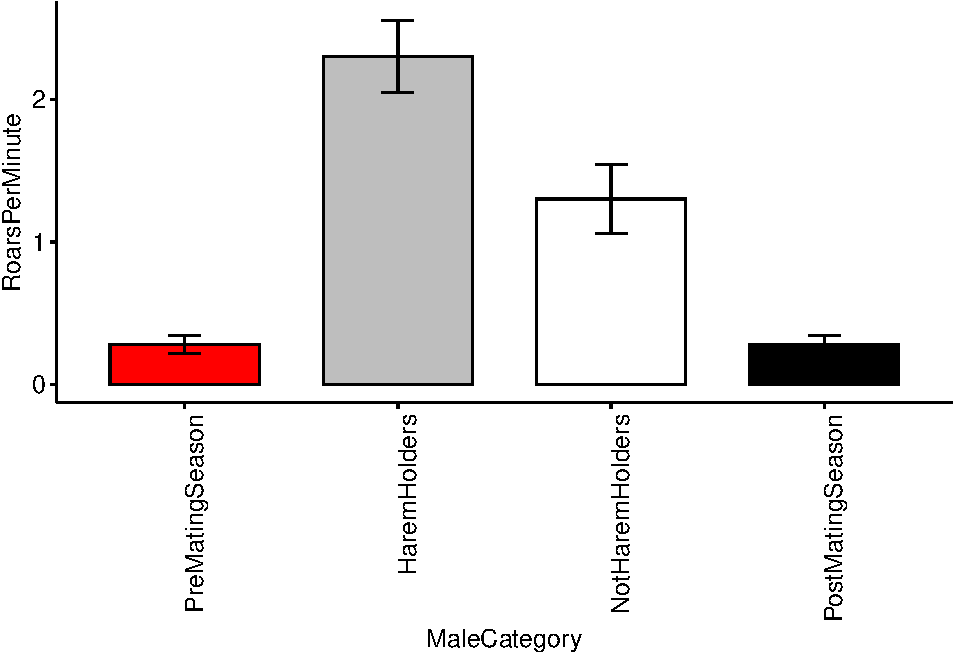
\includegraphics{behaviouR-R-package-tutorials_files/figure-latex/unnamed-chunk-10-1.pdf}

\emph{Please answer the following questions:}

Question 3. How do you interpret the barplot figure?

Question 4. Visit this site (\url{http://www.stat.columbia.edu/~tzheng/files/Rcolor.pdf}) and change the colors of the plot. Hint: change `palette = c('red',`gray',`white',`black')`to 'palette = c('color1',`color2',`color3',`color4')'.

\hypertarget{part-3.-categorical-and-continuous-data}{%
\section*{Part 3. Categorical and continuous data}\label{part-3.-categorical-and-continuous-data}}
\addcontentsline{toc}{section}{Part 3. Categorical and continuous data}

Continuous data represent numerical measurements, and when both our variables of interest are continuous we can plot them in a different way.

For this example we will consider the relationship between male red deer body weight (in kilograms) and male reproductive success (which is estimated by the number of days that he associated with females during the breeding season).

Below we have a function that will simulate data for us, and we can specify the level of correlation.

We also assign a mean body weight for males in our population. We can also change the male reproductive success value. The starting values that we will use are from Reby \& McComb 2003.

\begin{Shaded}
\begin{Highlighting}[]
\NormalTok{## Lab 1c. Categorical and continuous data}
\CommentTok{# This is the function that simulates our data. N is the number of individuals,   }
\CommentTok{# CorrelationCoefficient tells us how correlated our data are,  }
\CommentTok{# MaleMeanBodyWeight is the mean body weight of males in our population and }
\CommentTok{# MeanFemalesInHarem is the mean number of females in the harem.}
\NormalTok{MaleRedDeerDF <-}\StringTok{ }\KeywordTok{CorrelatedDataSimulationFunction}\NormalTok{(}\DataTypeTok{N=}\DecValTok{100}\NormalTok{, }
                                                  \DataTypeTok{CorrelationCoefficient=} \FloatTok{0.45}\NormalTok{,}
                                                  \DataTypeTok{MaleMeanBodyWeight =} \DecValTok{125}\NormalTok{,}
                                                  \DataTypeTok{MaleReproductiveSuccess =} \DecValTok{3}\NormalTok{)}

\CommentTok{# We can check the output}
\KeywordTok{head}\NormalTok{(MaleRedDeerDF)}
\end{Highlighting}
\end{Shaded}

\begin{verbatim}
##   MaleBodyWeight MaleReproductiveSuccess
## 1       125.2576                3.466009
## 2       125.1888                1.658102
## 3       124.7266                2.858253
## 4       124.1372                2.455370
## 5       125.4283                1.643711
## 6       124.3844                2.272255
\end{verbatim}

Now we plot the data the data as before, but this time we make a scatterplot

\begin{Shaded}
\begin{Highlighting}[]
\CommentTok{# Make a scatterplot of the data.}
\KeywordTok{ggscatter}\NormalTok{(}\DataTypeTok{data=}\NormalTok{MaleRedDeerDF,}\DataTypeTok{x=}\StringTok{'MaleBodyWeight'}\NormalTok{,}\DataTypeTok{y=}\StringTok{'MaleReproductiveSuccess'}\NormalTok{)}
\end{Highlighting}
\end{Shaded}

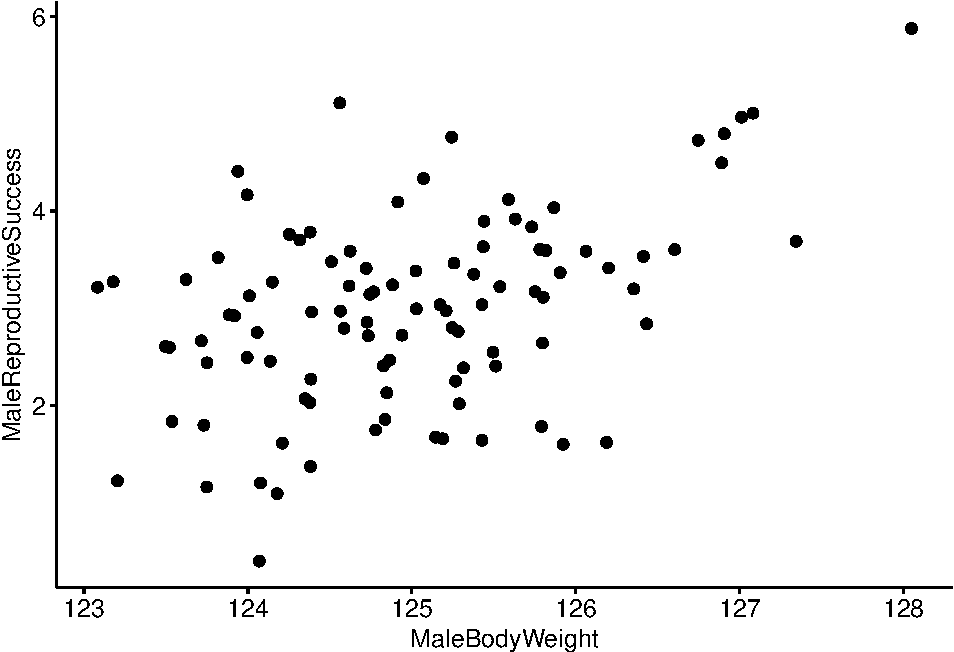
\includegraphics{behaviouR-R-package-tutorials_files/figure-latex/unnamed-chunk-12-1.pdf}

It looks like there is a correlation between our two variables, but it would be better visualized with a trend line. We can do that by including add=`reg.line'.

\begin{Shaded}
\begin{Highlighting}[]
\CommentTok{# Make a scatterplot with a trendline.}
\KeywordTok{ggscatter}\NormalTok{(}\DataTypeTok{data=}\NormalTok{MaleRedDeerDF,}\DataTypeTok{x=}\StringTok{'MaleBodyWeight'}\NormalTok{,}\DataTypeTok{y=}\StringTok{'MaleReproductiveSuccess'}\NormalTok{,}
          \DataTypeTok{add=}\StringTok{'reg.line'}\NormalTok{)}
\end{Highlighting}
\end{Shaded}

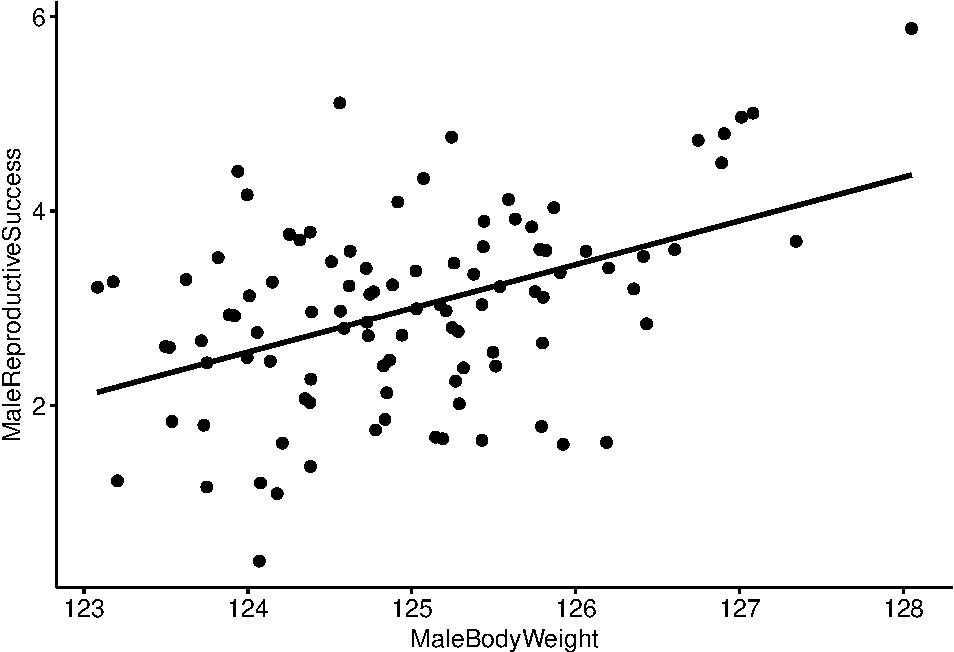
\includegraphics{behaviouR-R-package-tutorials_files/figure-latex/unnamed-chunk-13-1.pdf}

Now we can use R to create a linear model to quantitatively investigate the relationship between our two variables. Linear models describe the relationship of a continuous variable (in this case `MaleReproductiveSuccess') as a function of predictor variable(s). In the linear model below we are interested in the relationship between MaleBodyWeight and MaleReproductiveSuccess.

\begin{Shaded}
\begin{Highlighting}[]
\CommentTok{# Create a linear model where MaleBodyWeight is the independent variable}
\CommentTok{# and FemalesInHarem is the dependent variable.}
\NormalTok{MaleDeerModel <-}\StringTok{ }\KeywordTok{lm}\NormalTok{(MaleReproductiveSuccess }\OperatorTok{~}\StringTok{ }\NormalTok{MaleBodyWeight,}\DataTypeTok{data=}\NormalTok{MaleRedDeerDF)}
\end{Highlighting}
\end{Shaded}

We can look at the output of the model and we see that our coefficient for MaleBodyWeight is 0.45. We interpret this to mean that for every 1 kg increase in male body mass, we would expect to see a 0.45 increase in the reproductive success of the male. Since we simulated population so that there would be a correlation 0.45 between our two variables we already knew that this would be the outcome.

\begin{Shaded}
\begin{Highlighting}[]
\CommentTok{# We can look at the output of the model  }
\NormalTok{MaleDeerModel}
\end{Highlighting}
\end{Shaded}

\begin{verbatim}
## 
## Call:
## lm(formula = MaleReproductiveSuccess ~ MaleBodyWeight, data = MaleRedDeerDF)
## 
## Coefficients:
##    (Intercept)  MaleBodyWeight  
##         -53.25            0.45
\end{verbatim}

There are many ways that we can test whether the results of our model are reliable. A common way is through the use of p-values; a somewhat more intuitive way is through the use of model comparison using Akaike information criterion (AIC). AIC provides an estimate of how well the model fits the data.

NOTE: AIC can be used to compare two our more models created using the same dataset, but the relative AIC values are what is important, and you must use the same data for all models.

We will set up two models for this exercise. Our first model will be our 'null'model which does not include MaleBodyWeight as a predictor. Our next model will be our model of interest that does contain MaleBodyWeight as a predictor.

\begin{Shaded}
\begin{Highlighting}[]
\CommentTok{# Create a null model and a model with MaleBodyWeight as a predictor.}
\NormalTok{MaleDeerNull <-}\StringTok{ }\KeywordTok{lm}\NormalTok{(MaleReproductiveSuccess }\OperatorTok{~}\StringTok{ }\DecValTok{1}\NormalTok{, }\DataTypeTok{data=}\NormalTok{MaleRedDeerDF)}
\NormalTok{MaleDeerModel <-}\StringTok{ }\KeywordTok{lm}\NormalTok{(MaleReproductiveSuccess }\OperatorTok{~}\StringTok{ }\NormalTok{MaleBodyWeight,}\DataTypeTok{data=}\NormalTok{MaleRedDeerDF)}
\end{Highlighting}
\end{Shaded}

We can now use a function created to compare models using a modified version of AIC (adjusted for small sample sizes).

\begin{Shaded}
\begin{Highlighting}[]
\CommentTok{# Compare models using AIC.}
\NormalTok{bbmle}\OperatorTok{::}\KeywordTok{AICctab}\NormalTok{(MaleDeerModel,MaleDeerNull, }\DataTypeTok{weights=}\NormalTok{T)}
\end{Highlighting}
\end{Shaded}

\begin{verbatim}
##               dAICc df weight
## MaleDeerModel  0.0  3  1     
## MaleDeerNull  20.5  2  <0.001
\end{verbatim}

NOTE: In this example case the model which contains MaleBodyWeight is ranked higher. We interpret this to mean that there is a reliably positive relationship between MaleBodyWeight and MaleReproductiveSuccess. In other words, as male body weight increases we see an increase in his reproductive success.

\emph{Please answer the following questions:}

Question 5a. What happens when you change the correlation coefficent from 0.45 to a much smaller number and re-run the code?

Question 5b. What about when you change it to a much bigger number?

\hypertarget{part-4.-multivariate-data}{%
\section*{Part 4. Multivariate data}\label{part-4.-multivariate-data}}
\addcontentsline{toc}{section}{Part 4. Multivariate data}

In some cases we have multiple measurements of different variables from the same individual; in this case our data would be considered `multivariate'.

Lets create a toy dataset of red deer, sika deer and red x sika hybrid vocalizations (based on Long et al.~1998). We will simulate four vocalizations per individual and we will measure three aspects of the vocalizations- the duration, the minimum frequency and the maximum frequency of the vocalization. We will then visualize our data using principal component analysis (PCA). PCA is a commonly used data reduction technique.

For more information see \url{https://www.nature.com/articles/nmeth.4346.pdf}.

\begin{Shaded}
\begin{Highlighting}[]
\NormalTok{## Lab 1d. Multivariate data}
\CommentTok{# Just as before we load our data}
\KeywordTok{data}\NormalTok{(}\StringTok{"DeerSpeciesAcousticFeatures"}\NormalTok{)}

\CommentTok{# Check the structure}
\KeywordTok{head}\NormalTok{(DeerSpeciesAcousticFeatures)}
\end{Highlighting}
\end{Shaded}

\begin{verbatim}
##   Duration MinFrequency MaxFrequency   Class
## 1       15           50          125 RedDeer
## 2       14           49          127 RedDeer
## 3       12           51          126 RedDeer
## 4       13           52          127 RedDeer
## 5       17           35          125 Hybrids
## 6       19           37          126 Hybrids
\end{verbatim}

Now we run the PCA. Note: You can only do PCA on numeric data, so we remove the class category.

\begin{Shaded}
\begin{Highlighting}[]
\CommentTok{# Here is our modified dataset that we will use for PCA}
\NormalTok{DeerSpeciesAcousticFeatures[,}\OperatorTok{-}\KeywordTok{c}\NormalTok{(}\DecValTok{4}\NormalTok{)] }
\end{Highlighting}
\end{Shaded}

\begin{verbatim}
##    Duration MinFrequency MaxFrequency
## 1        15           50          125
## 2        14           49          127
## 3        12           51          126
## 4        13           52          127
## 5        17           35          125
## 6        19           37          126
## 7        15           34          123
## 8        16           32          127
## 9        21           20          125
## 10       22           20          126
## 11       23           21          124
## 12       20           25          127
\end{verbatim}

\begin{Shaded}
\begin{Highlighting}[]
\CommentTok{# Run the PCA using the 'princomp' function}
\NormalTok{DeerSpeciesAcousticFeaturesPCA <-}\StringTok{ }\KeywordTok{princomp}\NormalTok{(DeerSpeciesAcousticFeatures[,}\OperatorTok{-}\KeywordTok{c}\NormalTok{(}\DecValTok{4}\NormalTok{)])}
\end{Highlighting}
\end{Shaded}

Then we will plot the results
NOTE: each point represents one roar and the colors represent the class category.

\begin{Shaded}
\begin{Highlighting}[]
\CommentTok{# Plot the results of our PCA.}
\NormalTok{ggplot2}\OperatorTok{::}\KeywordTok{autoplot}\NormalTok{(DeerSpeciesAcousticFeaturesPCA, }\DataTypeTok{data =}\NormalTok{ DeerSpeciesAcousticFeatures, }\DataTypeTok{colour =} \StringTok{'Class'}\NormalTok{,}
         \DataTypeTok{loadings =} \OtherTok{FALSE}\NormalTok{)}\OperatorTok{+}\KeywordTok{theme_bw}\NormalTok{()}
\end{Highlighting}
\end{Shaded}

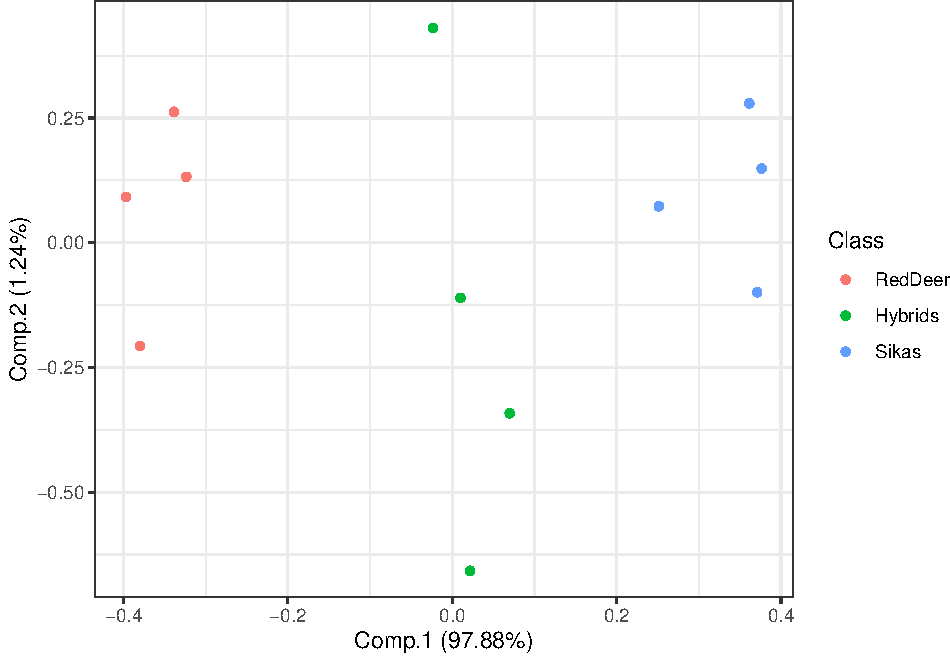
\includegraphics{behaviouR-R-package-tutorials_files/figure-latex/unnamed-chunk-20-1.pdf}

What if we are interested in which features best distinguish between our groups?
We can visualize this using the following code:

\begin{Shaded}
\begin{Highlighting}[]
\CommentTok{# Plot the PCA with arrows indicating which features are important for distinguishing between groups}
\NormalTok{ggplot2}\OperatorTok{::}\KeywordTok{autoplot}\NormalTok{(DeerSpeciesAcousticFeaturesPCA, }\DataTypeTok{data =}\NormalTok{ DeerSpeciesAcousticFeatures, }\DataTypeTok{colour =} \StringTok{'Class'}\NormalTok{,}
         \DataTypeTok{loadings =} \OtherTok{TRUE}\NormalTok{, }\DataTypeTok{loadings.colour =} \StringTok{'red'}\NormalTok{,}
         \DataTypeTok{loadings.label =} \OtherTok{TRUE}\NormalTok{,}
         \DataTypeTok{loadings.label.size =} \DecValTok{5}\NormalTok{)}\OperatorTok{+}\KeywordTok{theme_bw}\NormalTok{()}
\end{Highlighting}
\end{Shaded}

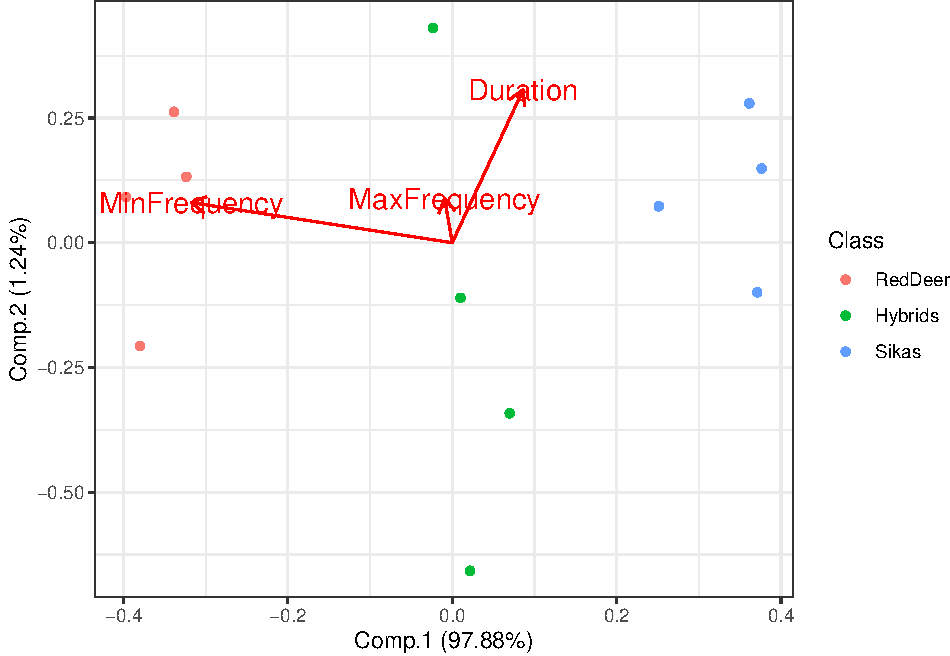
\includegraphics{behaviouR-R-package-tutorials_files/figure-latex/unnamed-chunk-21-1.pdf}

This shows that the feature that best distinguishes between red deer and sika is the minimum frequency of their vocalizations. If you look on the x-axis (Comp.1) you can see that there is a substantial amount of separation between these groups.

\emph{Please answer the following questions:}

Question 6. In your own words, explain why we would want to use PCA for data visualization? What can we learn about the data when it is visualized this way?

\hypertarget{computer-lab-2.-activity-budgets-and-ethograms}{%
\chapter*{Computer Lab 2. Activity Budgets and Ethograms}\label{computer-lab-2.-activity-budgets-and-ethograms}}
\addcontentsline{toc}{chapter}{Computer Lab 2. Activity Budgets and Ethograms}

\begin{center}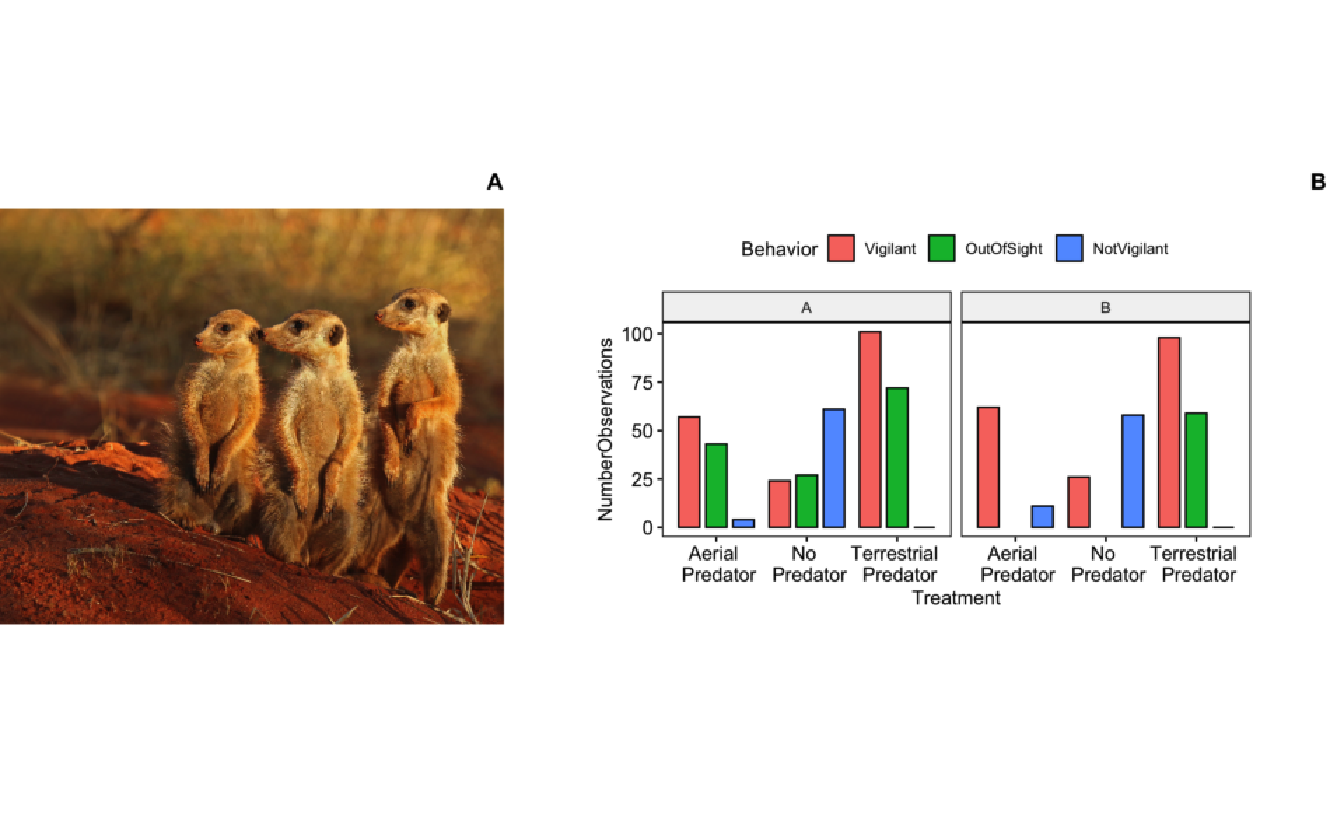
\includegraphics{behaviouR-R-package-tutorials_files/figure-latex/unnamed-chunk-22-1} \end{center}

\emph{Background}\\
In this lab you will continue to become familiar with the ways that we visualize and analyze behavioral data. For this lab I assume students have conducted Field Labs 1 and 2, so you should be familiar with how focal behavioral data are collected. Field Lab 1 data collection involves observation of animals in your own backyard and the creation of an ethogram. For Field Lab 2 data students learn how to collect focal data and scan data using meerkat videos following the methods outlined in: Hammond 2019, Vigilance behaviour in meerkats, ASAB Education.

\emph{Goals of the exercises}\\
The main goal(s) of today's lab are to:\\
1) Enter and visualize your ethogram data\\
2) Calculate meerkat activity budgets
3) Compare inter-observer reliability from the meerkat data

\emph{Getting started}\\
First we need to load the relevant packages for our data analysis. Packages contain all the functions that are needed for data analysis.

\begin{Shaded}
\begin{Highlighting}[]
\KeywordTok{library}\NormalTok{(behaviouR)}
\KeywordTok{library}\NormalTok{(ggpubr)}
\end{Highlighting}
\end{Shaded}

\hypertarget{part-1.-enter-and-visualize-your-ethogram-data}{%
\section*{Part 1. Enter and visualize your ethogram data}\label{part-1.-enter-and-visualize-your-ethogram-data}}
\addcontentsline{toc}{section}{Part 1. Enter and visualize your ethogram data}

Here we will do an exploratory analysis of the ethograms that you created in Field Lab 1.
First we will use some simulated (or made up) data to create our ethogram. In R we call the objects that contain our data `dataframes'.

\begin{Shaded}
\begin{Highlighting}[]
\NormalTok{EthogramDF <-}\StringTok{ }
\StringTok{  }\KeywordTok{data.frame}\NormalTok{(}\DataTypeTok{Behavior=}\KeywordTok{c}\NormalTok{(}\StringTok{'Resting'}\NormalTok{,}\StringTok{'Locomotion'}\NormalTok{,}\StringTok{'Foraging'}\NormalTok{,}\StringTok{'Calling'}\NormalTok{,}\StringTok{'Playing'}\NormalTok{,}\StringTok{'Other'}\NormalTok{),}
                 \DataTypeTok{TimesObserved=}\KeywordTok{c}\NormalTok{(}\DecValTok{5}\NormalTok{,}\DecValTok{7}\NormalTok{,}\DecValTok{3}\NormalTok{,}\DecValTok{21}\NormalTok{,}\DecValTok{1}\NormalTok{,}\DecValTok{0}\NormalTok{))}
\end{Highlighting}
\end{Shaded}

If you run the object `EthogramDF' you should see your table:

\begin{Shaded}
\begin{Highlighting}[]
\NormalTok{EthogramDF}
\end{Highlighting}
\end{Shaded}

\begin{verbatim}
##     Behavior TimesObserved
## 1    Resting             5
## 2 Locomotion             7
## 3   Foraging             3
## 4    Calling            21
## 5    Playing             1
## 6      Other             0
\end{verbatim}

A common command to check data structure is `str'. Here we can see our dataframe has two variables:`Behavior' and `TimesObserved'.

\begin{Shaded}
\begin{Highlighting}[]
\KeywordTok{str}\NormalTok{(EthogramDF)}
\end{Highlighting}
\end{Shaded}

\begin{verbatim}
## 'data.frame':    6 obs. of  2 variables:
##  $ Behavior     : Factor w/ 6 levels "Calling","Foraging",..: 6 3 2 1 5 4
##  $ TimesObserved: num  5 7 3 21 1 0
\end{verbatim}

Now we can make a barplot to visualize our results using the `ggpubr' package

\begin{Shaded}
\begin{Highlighting}[]
\KeywordTok{ggbarplot}\NormalTok{(}\DataTypeTok{data=}\NormalTok{EthogramDF, }\DataTypeTok{x=}\StringTok{'Behavior'}\NormalTok{, }\DataTypeTok{y=}\StringTok{'TimesObserved'}\NormalTok{,}\DataTypeTok{fill=}\StringTok{'grey'}\NormalTok{)}
\end{Highlighting}
\end{Shaded}

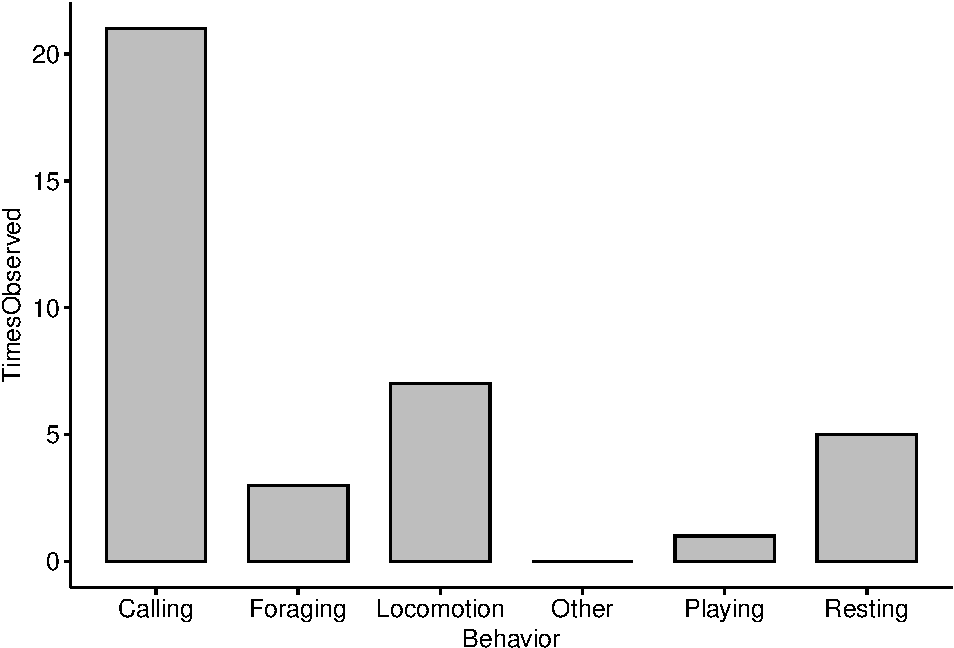
\includegraphics{behaviouR-R-package-tutorials_files/figure-latex/unnamed-chunk-27-1.pdf}

In the space below I want you to add in your own ethogram categories and create a plot based on the ethogram you created in Field lab 1.

Change the Behavior categories (i.e.~Category1) to the categories you used in your ethogram and the TimesObserved values to the actual values you recorded

\begin{Shaded}
\begin{Highlighting}[]
\NormalTok{EthogramDFupdated <-}\StringTok{ }\KeywordTok{data.frame}\NormalTok{(}\DataTypeTok{Behavior=}\KeywordTok{c}\NormalTok{(}\StringTok{'Category1'}\NormalTok{,}\StringTok{'Category2'}\NormalTok{,}\StringTok{'Category3'}\NormalTok{,}
                                           \StringTok{'Category4'}\NormalTok{,}\StringTok{'Category5'}\NormalTok{,}\StringTok{'Category6'}\NormalTok{),}
                         \DataTypeTok{TimesObserved=}\KeywordTok{c}\NormalTok{(}\DecValTok{1}\NormalTok{,}\DecValTok{2}\NormalTok{,}\DecValTok{3}\NormalTok{,}\DecValTok{4}\NormalTok{,}\DecValTok{5}\NormalTok{,}\DecValTok{6}\NormalTok{))}
\end{Highlighting}
\end{Shaded}

If you run the object you should see your dataframe

\begin{Shaded}
\begin{Highlighting}[]
\KeywordTok{head}\NormalTok{(EthogramDFupdated)}
\end{Highlighting}
\end{Shaded}

\begin{verbatim}
##    Behavior TimesObserved
## 1 Category1             1
## 2 Category2             2
## 3 Category3             3
## 4 Category4             4
## 5 Category5             5
## 6 Category6             6
\end{verbatim}

NOTE: Your plot will look different than this as you will enter your own data above!

\begin{Shaded}
\begin{Highlighting}[]
\KeywordTok{ggbarplot}\NormalTok{(}\DataTypeTok{data=}\NormalTok{EthogramDFupdated, }\DataTypeTok{x=}\StringTok{'Behavior'}\NormalTok{, }\DataTypeTok{y=}\StringTok{'TimesObserved'}\NormalTok{,}\DataTypeTok{fill=}\StringTok{'grey'}\NormalTok{,}\DataTypeTok{xtickslab.rt =} \DecValTok{90}\NormalTok{)}
\end{Highlighting}
\end{Shaded}

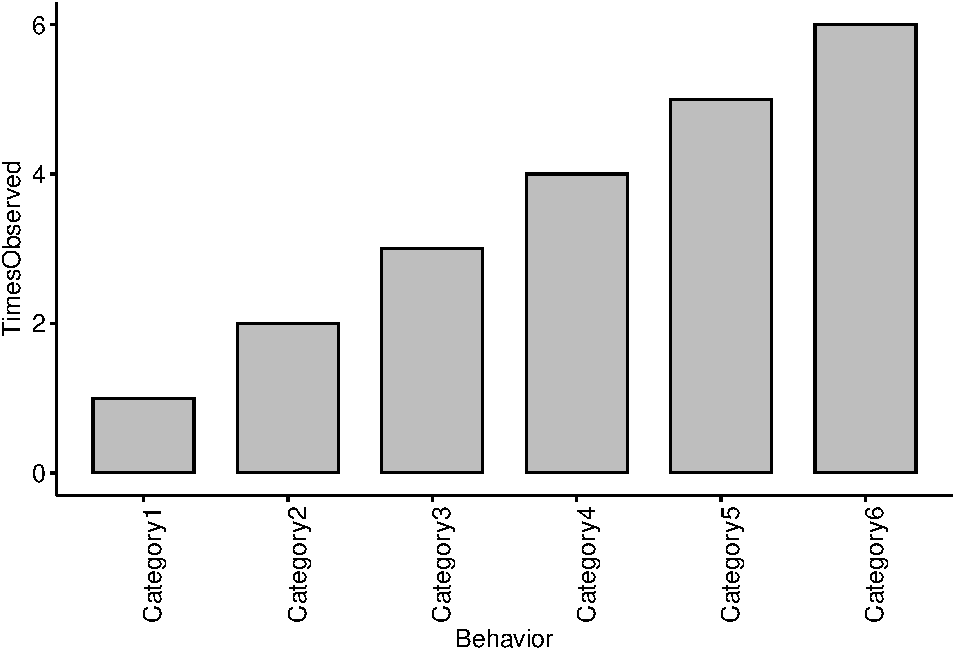
\includegraphics{behaviouR-R-package-tutorials_files/figure-latex/unnamed-chunk-30-1.pdf}

\textbf{Question 1}\\
\emph{Change the code to reflect the categories you used in your ethogram and change the TimesObserved values to the actual values you recorded. NOTE: You may need to add more categories if your ethogram had more than six. What trends did you notice in terms of behaviors observed?}

\hypertarget{part-2.-calculate-meerkat-activity-budgets.}{%
\section*{Part 2. Calculate meerkat activity budgets.}\label{part-2.-calculate-meerkat-activity-budgets.}}
\addcontentsline{toc}{section}{Part 2. Calculate meerkat activity budgets.}

Our previous ethograms only included counts of different behaviors that we observed, but we did not standardize our results in any way. Activity budgets give an indication of how much time an animal spends doing each activity; these are generally expressed as percentages.

First we need to import the data. If you are using RStudio Cloud you can import your data by clicking the `upload' button and find the datasheet saved on your computer. You can then use the following lines to read your data into R.

\begin{Shaded}
\begin{Highlighting}[]
\NormalTok{MeerkatFocalData <-}\StringTok{ }\KeywordTok{read.csv}\NormalTok{(}\StringTok{'MeerkatFocalData.csv'}\NormalTok{)}
\NormalTok{MeerkatScanData <-}\StringTok{ }\KeywordTok{read.csv}\NormalTok{(}\StringTok{'MeerkatScanData.csv'}\NormalTok{)}
\end{Highlighting}
\end{Shaded}

We also have sample data saved in the package so we can load that using the following code

\begin{Shaded}
\begin{Highlighting}[]
\KeywordTok{data}\NormalTok{(}\StringTok{"MeerkatFocalData"}\NormalTok{)}
\KeywordTok{data}\NormalTok{(}\StringTok{"MeerkatScanData"}\NormalTok{)}
\end{Highlighting}
\end{Shaded}

NOTE: If you are using your own data you will want to keep the file names the exact same or R won't be able to find the data.
Let's check the structure of our data.

\begin{Shaded}
\begin{Highlighting}[]
\KeywordTok{str}\NormalTok{(MeerkatFocalData)}
\end{Highlighting}
\end{Shaded}

\begin{verbatim}
## 'data.frame':    28 obs. of  6 variables:
##  $ StartTimeMin            : int  0 1 2 3 3 4 4 5 5 5 ...
##  $ StartTimeSec            : int  30 20 40 0 30 0 20 0 30 50 ...
##  $ BehaviorCode            : Factor w/ 5 levels "Drinking","Eating",..: 2 4 1 1 2 3 2 3 3 3 ...
##  $ TimeSeconds             : int  30 80 160 180 210 240 260 300 330 350 ...
##  $ SecondsEngagedinBehavior: int  30 50 80 20 30 30 20 40 30 20 ...
##  $ Partner                 : Factor w/ 2 levels "A","B": 1 1 1 1 1 1 1 1 1 1 ...
\end{verbatim}

Then we calcuate the total number of seconds for each behavior. There are many different ways that we can summarize our data using R, but we will use the package `dplyr'.

Here we take the sum for each unique behavior and return it

\begin{Shaded}
\begin{Highlighting}[]
\NormalTok{MeerkatFocalData }\OperatorTok\StringTok{ }
\StringTok{  }\NormalTok{dplyr}\OperatorTok{::}\KeywordTok{group_by}\NormalTok{(BehaviorCode) }\OperatorTok\StringTok{ }
\StringTok{  }\NormalTok{dplyr}\OperatorTok{::}\KeywordTok{summarise}\NormalTok{(}\DataTypeTok{TotalSeconds =} \KeywordTok{sum}\NormalTok{(SecondsEngagedinBehavior))}
\end{Highlighting}
\end{Shaded}

\begin{verbatim}
## # A tibble: 5 x 2
##   BehaviorCode TotalSeconds
##   <fct>               <int>
## 1 Drinking              200
## 2 Eating                150
## 3 Foraging              350
## 4 Locomotion            250
## 5 Sentry                240
\end{verbatim}

Then we need to save the output as an R object

\begin{Shaded}
\begin{Highlighting}[]
\NormalTok{MeerkatFocalDataSummary <-}\StringTok{ }\NormalTok{MeerkatFocalData }\OperatorTok\StringTok{ }
\StringTok{  }\NormalTok{dplyr}\OperatorTok{::}\KeywordTok{group_by}\NormalTok{(BehaviorCode) }\OperatorTok\StringTok{ }
\StringTok{  }\NormalTok{dplyr}\OperatorTok{::}\KeywordTok{summarise}\NormalTok{(}\DataTypeTok{TotalSeconds =} \KeywordTok{sum}\NormalTok{(SecondsEngagedinBehavior))}
\end{Highlighting}
\end{Shaded}

Now we need to standardize for our total observation time. We divide by 600 because our video was 10 minutes (or 600 seconds) long.

\begin{Shaded}
\begin{Highlighting}[]
\NormalTok{MeerkatFocalDataSummary}\OperatorTok{$}\NormalTok{ActivityBudget <-}\StringTok{ }\NormalTok{MeerkatFocalDataSummary}\OperatorTok{$}\NormalTok{TotalSeconds}\OperatorTok{/}\DecValTok{600}\OperatorTok{*}\DecValTok{100}
\end{Highlighting}
\end{Shaded}

Now let's plot our results!
NOTE: The example here is using fake data.

\begin{Shaded}
\begin{Highlighting}[]
\KeywordTok{ggbarplot}\NormalTok{(}\DataTypeTok{data=}\NormalTok{MeerkatFocalDataSummary,}\DataTypeTok{x=}\StringTok{'BehaviorCode'}\NormalTok{,}\DataTypeTok{y=}\StringTok{'ActivityBudget'}\NormalTok{,}\DataTypeTok{fill=}\StringTok{'grey'}\NormalTok{)}\OperatorTok{+}\KeywordTok{ylab}\NormalTok{(}\StringTok{'Percent of Time'}\NormalTok{)}
\end{Highlighting}
\end{Shaded}

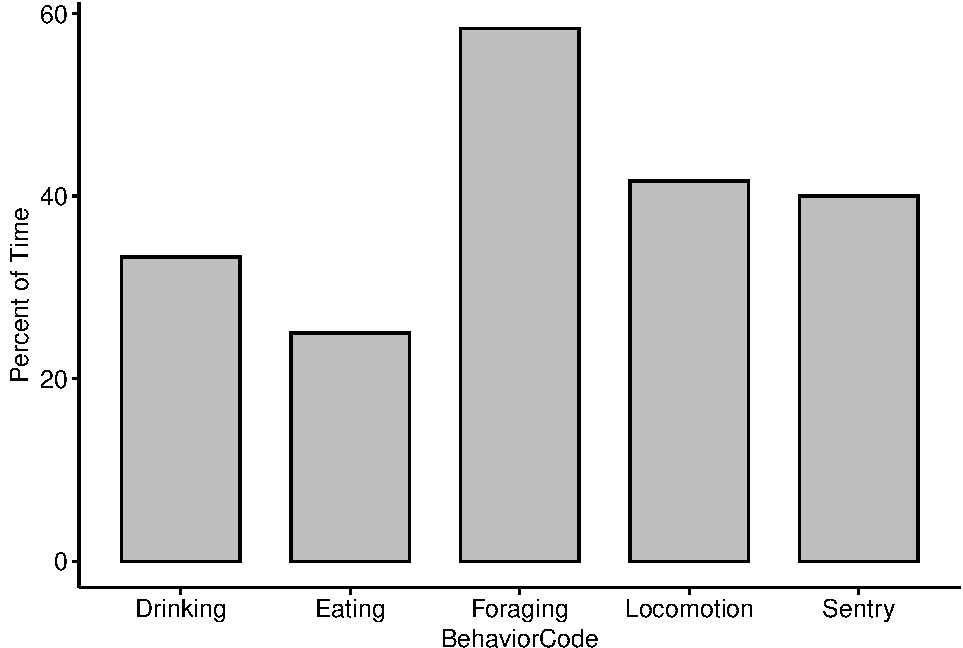
\includegraphics{behaviouR-R-package-tutorials_files/figure-latex/unnamed-chunk-37-1.pdf}

Now lets see if there were differences between you and your partner. We need to save the output as an R object, but this time including the sums by partner.

\begin{Shaded}
\begin{Highlighting}[]
\NormalTok{MeerkatFocalDataPartner <-}\StringTok{ }\NormalTok{MeerkatFocalData }\OperatorTok\StringTok{ }
\StringTok{  }\NormalTok{dplyr}\OperatorTok{::}\KeywordTok{group_by}\NormalTok{(BehaviorCode,Partner) }\OperatorTok\StringTok{ }
\StringTok{  }\NormalTok{dplyr}\OperatorTok{::}\KeywordTok{summarise}\NormalTok{(}\DataTypeTok{TotalSeconds =} \KeywordTok{sum}\NormalTok{(SecondsEngagedinBehavior))}
\end{Highlighting}
\end{Shaded}

Again, we divide by 600 because our video was 10 minutes (or 600 seconds) long. We then multiply by 100 so that we can report in percentages.

\begin{Shaded}
\begin{Highlighting}[]
\NormalTok{MeerkatFocalDataPartner}\OperatorTok{$}\NormalTok{ActivityBudget <-}\StringTok{ }\NormalTok{MeerkatFocalDataPartner}\OperatorTok{$}\NormalTok{TotalSeconds}\OperatorTok{/}\DecValTok{600}\OperatorTok{*}\DecValTok{100}
\end{Highlighting}
\end{Shaded}

Now we compare our data with our partner's. Note that there are two new lines in the code below. The fill argument tells R which category or factor to use to color the bars. The position argument tells R to place the bars side-by-side.

\begin{Shaded}
\begin{Highlighting}[]
\KeywordTok{ggbarplot}\NormalTok{(}\DataTypeTok{data=}\NormalTok{MeerkatFocalDataPartner,}\DataTypeTok{x=}\StringTok{'BehaviorCode'}\NormalTok{,}\DataTypeTok{y=}\StringTok{'ActivityBudget'}\NormalTok{, }\DataTypeTok{fill=}\StringTok{'Partner'}\NormalTok{,}
          \DataTypeTok{position =} \KeywordTok{position_dodge}\NormalTok{(}\FloatTok{0.9}\NormalTok{))}\OperatorTok{+}\KeywordTok{ylab}\NormalTok{(}\StringTok{'Percent of Time'}\NormalTok{)}
\end{Highlighting}
\end{Shaded}

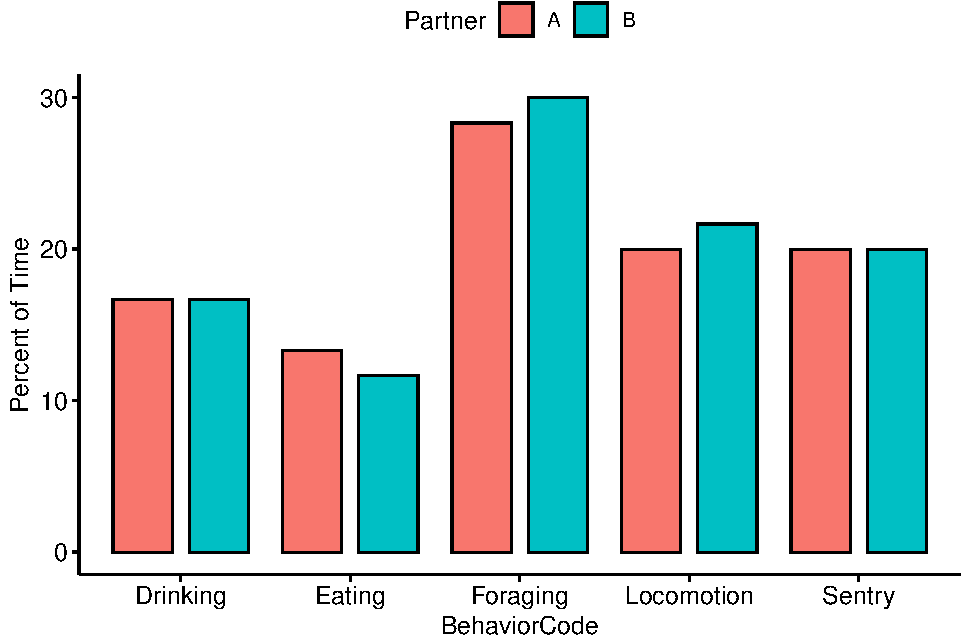
\includegraphics{behaviouR-R-package-tutorials_files/figure-latex/unnamed-chunk-40-1.pdf}

\textbf{Question 3}.\\
\emph{Were there any noticeable differences between you and your partner's activity budgets?}

\hypertarget{part-3.-scan-sampling-and-inter-observer-reliability.}{%
\section*{Part 3. Scan sampling and inter-observer reliability.}\label{part-3.-scan-sampling-and-inter-observer-reliability.}}
\addcontentsline{toc}{section}{Part 3. Scan sampling and inter-observer reliability.}

Load your data as you did before, but this time upload the `MeerkatScanData.csv' file.

Check the structure of our data. If we use `head' it will return the first few rows of our dataframe.

\begin{Shaded}
\begin{Highlighting}[]
\KeywordTok{head}\NormalTok{(MeerkatScanData)}
\end{Highlighting}
\end{Shaded}

\begin{verbatim}
##   Time Vigilant NotVigilant OutOfSight  Treatment Partner
## 1   10        1           3          2 NoPredator       A
## 2   20        1           5          0 NoPredator       A
## 3   30        2           3          1 NoPredator       A
## 4   40        2           4          0 NoPredator       A
## 5   50        1           4          1 NoPredator       A
## 6   60        2           4          1 NoPredator       A
\end{verbatim}

For this analysis the `Time' column isn't needed so we can remove it; It is the first column so we use 1 in the code below.

\begin{Shaded}
\begin{Highlighting}[]
\NormalTok{MeerkatScanData <-MeerkatScanData[,}\OperatorTok{-}\KeywordTok{c}\NormalTok{(}\DecValTok{1}\NormalTok{)]}
\end{Highlighting}
\end{Shaded}

R deals with blanks in dataframes by converting them to `NA'. This is useful for some cases, but we want to convert our blanks to zeros using the following code.

\begin{Shaded}
\begin{Highlighting}[]
\NormalTok{MeerkatScanData[}\KeywordTok{is.na}\NormalTok{(MeerkatScanData)] <-}\StringTok{ }\DecValTok{0}
\end{Highlighting}
\end{Shaded}

Here we take the sum for each unique behavior and return it.

\begin{Shaded}
\begin{Highlighting}[]
\NormalTok{MeerkatScanData }\OperatorTok\StringTok{ }
\StringTok{  }\NormalTok{dplyr}\OperatorTok{::}\KeywordTok{group_by}\NormalTok{(Treatment) }\OperatorTok\StringTok{ }
\StringTok{  }\NormalTok{dplyr}\OperatorTok{::}\KeywordTok{summarise}\NormalTok{(}\DataTypeTok{Vigilant =} \KeywordTok{sum}\NormalTok{(Vigilant),}
                   \DataTypeTok{OutOfSight=}\KeywordTok{sum}\NormalTok{(OutOfSight),}
                   \DataTypeTok{NotVigilant=}\KeywordTok{sum}\NormalTok{(NotVigilant))}
\end{Highlighting}
\end{Shaded}

\begin{verbatim}
## # A tibble: 3 x 4
##   Treatment           Vigilant OutOfSight NotVigilant
##   <fct>                  <int>      <dbl>       <int>
## 1 AerialPredator           119         73          15
## 2 NoPredator                50         64         119
## 3 TerrestrialPredator      199        131           0
\end{verbatim}

We need to save the output as an R object

\begin{Shaded}
\begin{Highlighting}[]
\NormalTok{MeerkatScanDataSummary <-}\StringTok{ }\NormalTok{MeerkatScanData }\OperatorTok\StringTok{ }
\StringTok{  }\NormalTok{dplyr}\OperatorTok{::}\KeywordTok{group_by}\NormalTok{(Treatment,Partner) }\OperatorTok\StringTok{ }
\StringTok{  }\NormalTok{dplyr}\OperatorTok{::}\KeywordTok{summarise}\NormalTok{(}\DataTypeTok{Vigilant =} \KeywordTok{sum}\NormalTok{(Vigilant),}
                   \DataTypeTok{OutOfSight=}\KeywordTok{sum}\NormalTok{(OutOfSight),}
                   \DataTypeTok{NotVigilant=}\KeywordTok{sum}\NormalTok{(NotVigilant))}
\end{Highlighting}
\end{Shaded}

There are many functions in R that allow us to change the format of our data. This one changes the format to one that is more easily used by `ggpubr'

\begin{Shaded}
\begin{Highlighting}[]
\NormalTok{MeerkatScanDataSummaryLong <-}\StringTok{ }\NormalTok{reshape2}\OperatorTok{::}\KeywordTok{melt}\NormalTok{(MeerkatScanDataSummary, }\DataTypeTok{id.vars=}\KeywordTok{c}\NormalTok{(}\StringTok{"Treatment"}\NormalTok{, }\StringTok{"Partner"}\NormalTok{))}
\KeywordTok{str}\NormalTok{(MeerkatScanDataSummaryLong)}
\end{Highlighting}
\end{Shaded}

\begin{verbatim}
## 'data.frame':    18 obs. of  4 variables:
##  $ Treatment: Factor w/ 3 levels "AerialPredator",..: 1 1 2 2 3 3 1 1 2 2 ...
##  $ Partner  : Factor w/ 2 levels "A","B": 1 2 1 2 1 2 1 2 1 2 ...
##  $ variable : Factor w/ 3 levels "Vigilant","OutOfSight",..: 1 1 1 1 1 1 2 2 2 2 ...
##  $ value    : num  57 62 24 26 101 98 43 30 27 37 ...
\end{verbatim}

Now we change the column names so they are better for plotting

\begin{Shaded}
\begin{Highlighting}[]
\KeywordTok{colnames}\NormalTok{(MeerkatScanDataSummaryLong) <-}\StringTok{ }\KeywordTok{c}\NormalTok{(}\StringTok{'Treatment'}\NormalTok{,}\StringTok{'Partner'}\NormalTok{,}\StringTok{'Behavior'}\NormalTok{,}\StringTok{'NumberObservations'}\NormalTok{)}

\NormalTok{MeerkatScanDataSummaryLong}\OperatorTok{$}\NormalTok{Treatment <-}\StringTok{ }\NormalTok{plyr}\OperatorTok{::}\KeywordTok{revalue}\NormalTok{(MeerkatScanDataSummaryLong}\OperatorTok{$}\NormalTok{Treatment,}
                                                \KeywordTok{c}\NormalTok{(}\DataTypeTok{AerialPredator=}\StringTok{'Aerial }\CharTok{\textbackslash{}n}\StringTok{ Predator'}\NormalTok{,}
                                                  \DataTypeTok{NoPredator=}\StringTok{'No }\CharTok{\textbackslash{}n}\StringTok{ Predator'}\NormalTok{,}
                                                  \DataTypeTok{TerrestrialPredator=}\StringTok{'Terrestrial }\CharTok{\textbackslash{}n}\StringTok{ Predator'}\NormalTok{))}
\end{Highlighting}
\end{Shaded}

And now we can visually compare our results with our partners. Note that in order to separate the plots by partner we use facet.by = `Partner'.

\begin{Shaded}
\begin{Highlighting}[]
\KeywordTok{ggbarplot}\NormalTok{(}\DataTypeTok{data=}\NormalTok{MeerkatScanDataSummaryLong,}\DataTypeTok{x=}\StringTok{'Treatment'}\NormalTok{,}\DataTypeTok{y=}\StringTok{'NumberObservations'}\NormalTok{, }\DataTypeTok{fill=}\StringTok{'Behavior'}\NormalTok{,}
          \DataTypeTok{position =} \KeywordTok{position_dodge}\NormalTok{(}\FloatTok{0.9}\NormalTok{),}\DataTypeTok{facet.by =} \StringTok{'Partner'}\NormalTok{)}
\end{Highlighting}
\end{Shaded}

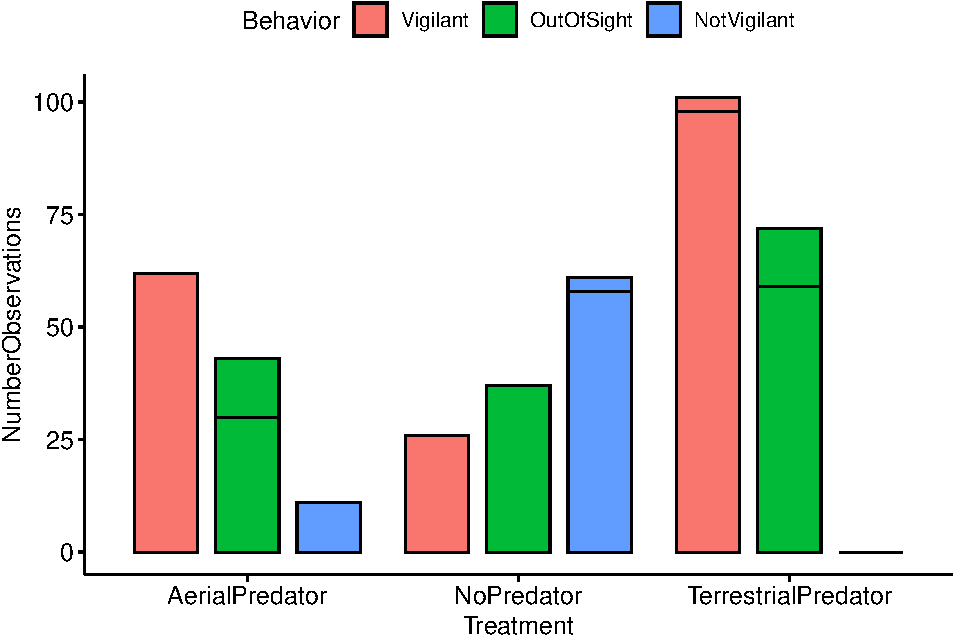
\includegraphics{behaviouR-R-package-tutorials_files/figure-latex/unnamed-chunk-48-1.pdf}

Now we want to calculate inter-observer reliablity.
NOTE: that you will want to change the A and B to the names you used in the datasheet

\begin{Shaded}
\begin{Highlighting}[]
\NormalTok{Partner1Data <-}\StringTok{ }\KeywordTok{subset}\NormalTok{(MeerkatScanData,Partner}\OperatorTok{==}\StringTok{'A'}\NormalTok{)}
\NormalTok{Partner1Data <-}\StringTok{ }\NormalTok{Partner1Data[,}\OperatorTok{-}\KeywordTok{c}\NormalTok{(}\DecValTok{5}\NormalTok{)] }\CommentTok{# We remove the 'Partner' column so that we only focus on scans}

\NormalTok{Partner2Data <-}\StringTok{ }\KeywordTok{subset}\NormalTok{(MeerkatScanData,Partner}\OperatorTok{==}\StringTok{'B'}\NormalTok{)}
\NormalTok{Partner2Data <-}\StringTok{ }\NormalTok{Partner2Data[,}\OperatorTok{-}\KeywordTok{c}\NormalTok{(}\DecValTok{5}\NormalTok{)] }\CommentTok{# We remove the 'Partner' column so that we only focus on scans}
\end{Highlighting}
\end{Shaded}

Reliability is often and most simply expressed as a correlation coefficient. A correlation of 1 means a perfect positive association between two sets of measurements, whereas a correlation of zero means the complete absence of a linear association. Reliability is generally calcuated for each category of behavior.

\begin{Shaded}
\begin{Highlighting}[]
\CommentTok{# Here we calculate reliability for vigilance}
\NormalTok{VigilantCorrelation <-}\StringTok{ }\KeywordTok{cor}\NormalTok{(Partner1Data}\OperatorTok{$}\NormalTok{Vigilant,Partner2Data}\OperatorTok{$}\NormalTok{Vigilant)}

\CommentTok{# Here we calculate reliability for vigilance}
\NormalTok{NotVigilantCorrelation <-}\StringTok{ }\KeywordTok{cor}\NormalTok{(Partner1Data}\OperatorTok{$}\NormalTok{NotVigilant,Partner2Data}\OperatorTok{$}\NormalTok{NotVigilant)}

\CommentTok{# Here we calculate reliability for out of sight}
\NormalTok{OutOfSightCorrelation <-}\StringTok{  }\KeywordTok{cor}\NormalTok{(Partner1Data}\OperatorTok{$}\NormalTok{OutOfSight,Partner2Data}\OperatorTok{$}\NormalTok{OutOfSight)}

\CommentTok{# Print the results}
\KeywordTok{cbind.data.frame}\NormalTok{(VigilantCorrelation,NotVigilantCorrelation,OutOfSightCorrelation)}
\end{Highlighting}
\end{Shaded}

\begin{verbatim}
##   VigilantCorrelation NotVigilantCorrelation OutOfSightCorrelation
## 1           0.9027009              0.9347273             0.7840471
\end{verbatim}

NOTE: The correlation values between you and your partner will be different!

\textbf{Question 4}.\\
\emph{What was the reliability (or correlation coefficent) between you and your partner for each of the different behavioral categories? What do you think lead to these differences? }

\hypertarget{computer-lab-3.-analyzing-acoustic-data}{%
\chapter*{Computer Lab 3. Analyzing Acoustic Data}\label{computer-lab-3.-analyzing-acoustic-data}}
\addcontentsline{toc}{chapter}{Computer Lab 3. Analyzing Acoustic Data}

\begin{verbatim}
## NULL
\end{verbatim}

\begin{verbatim}
## [1] "processing sound event 1 out of 13"
## [1] "processing sound event 2 out of 13"
## [1] "processing sound event 3 out of 13"
## [1] "processing sound event 4 out of 13"
## [1] "processing sound event 5 out of 13"
## [1] "processing sound event 6 out of 13"
## [1] "processing sound event 7 out of 13"
## [1] "processing sound event 8 out of 13"
## [1] "processing sound event 9 out of 13"
## [1] "processing sound event 10 out of 13"
## [1] "processing sound event 11 out of 13"
## [1] "processing sound event 12 out of 13"
## [1] "processing sound event 13 out of 13"
\end{verbatim}

\emph{Background}\\
In this lab you will become familiar with the ways that we analyze acoustic data. You will start by analyzing focal recordings and soundscapes from Southeast Asia, and you will then upload the data you collected for Field Lab 3 and do some prelminary analysis.

\emph{Goals of the exercises}\\
The main goal(s) of today's lab are to:\\
1) Create your own spectrograms\\
2) Learn how we use PCA to visualize differences in acoustic data\\
3) Upload and visualize your own data

\emph{Getting started}\\
First we need to load the relevant packages for our data analysis. Packages contain all the functions that are needed for data analysis.
First we load the required libraries

\begin{Shaded}
\begin{Highlighting}[]
\KeywordTok{library}\NormalTok{(behaviouR)}
\KeywordTok{library}\NormalTok{(ggfortify) }
\KeywordTok{library}\NormalTok{(ggplot2)}
\end{Highlighting}
\end{Shaded}

We need to do some data prep to work through the examples

\begin{Shaded}
\begin{Highlighting}[]
\CommentTok{# First you can check where your working directory is; this is where R will store the files locally}
\KeywordTok{getwd}\NormalTok{()}

\CommentTok{# Now we will create a file at this location called 'FocalRecordings'}
\KeywordTok{dir.create}\NormalTok{(}\KeywordTok{file.path}\NormalTok{(}\StringTok{'FocalRecordings'}\NormalTok{), }\DataTypeTok{showWarnings =} \OtherTok{FALSE}\NormalTok{)}

\CommentTok{# Now we will load the sound files that were in the R package}
\NormalTok{githubURL <-}\StringTok{'https://github.com/DenaJGibbon/behaviouRdata/raw/master/data/FocalRecordings.rda'}
\NormalTok{FocalRecordings <-}\StringTok{ }\KeywordTok{get}\NormalTok{(}\KeywordTok{load}\NormalTok{(}\KeywordTok{url}\NormalTok{(githubURL)))}

\CommentTok{# Let's check the structure}
\KeywordTok{head}\NormalTok{(FocalRecordings)}

\CommentTok{# Now we will save the recordings to the new folder you created}
\ControlFlowTok{for}\NormalTok{(a }\ControlFlowTok{in} \DecValTok{1}\OperatorTok{:}\KeywordTok{length}\NormalTok{(FocalRecordings))\{}
\NormalTok{  FileName <-}\StringTok{ }\NormalTok{FocalRecordings[[a]][}\DecValTok{1}\NormalTok{][[}\DecValTok{1}\NormalTok{]]}
\NormalTok{  WaveFile <-}\StringTok{ }\NormalTok{FocalRecordings[[a]][}\DecValTok{2}\NormalTok{][[}\DecValTok{1}\NormalTok{]]}
\NormalTok{  tuneR}\OperatorTok{::}\KeywordTok{writeWave}\NormalTok{(WaveFile, }\KeywordTok{paste}\NormalTok{(}\StringTok{"FocalRecordings/"}\NormalTok{,FileName,}\DataTypeTok{sep=}\StringTok{''}\NormalTok{))}
\NormalTok{\}}
\end{Highlighting}
\end{Shaded}

\hypertarget{part-1.-loading-a-sound-file-and-making-a-spectrogram}{%
\section*{Part 1. Loading a sound file and making a spectrogram}\label{part-1.-loading-a-sound-file-and-making-a-spectrogram}}
\addcontentsline{toc}{section}{Part 1. Loading a sound file and making a spectrogram}

First we want to check which files are in the folder
There are five gibbon female recordings and five great argus recordings.

\begin{Shaded}
\begin{Highlighting}[]
\KeywordTok{list.files}\NormalTok{(}\StringTok{"FocalRecordings"}\NormalTok{)}
\end{Highlighting}
\end{Shaded}

\begin{verbatim}
##  [1] "FemaleGibbon_1.wav" "FemaleGibbon_2.wav" "FemaleGibbon_3.wav"
##  [4] "FemaleGibbon_4.wav" "FemaleGibbon.wav"   "GreatArgus_1.wav"  
##  [7] "GreatArgus_2.wav"   "GreatArgus_3.wav"   "GreatArgus_4.wav"  
## [10] "MaleSolo_1.wav"     "MaleSolo_2.wav"     "MaleSolo_3.wav"    
## [13] "MaleSolo_4.wav"
\end{verbatim}

Now let's read in one of the files for further investigation. We do that with the function `readWave'. The .wav stands for `Waveform Audio File' and is a common format that scientists use to save their sound files.

\begin{Shaded}
\begin{Highlighting}[]
\NormalTok{GibbonWaveFile <-}\StringTok{ }\NormalTok{tuneR}\OperatorTok{::}\KeywordTok{readWave}\NormalTok{(}\StringTok{"FocalRecordings/FemaleGibbon_1.wav"}\NormalTok{)}
\end{Highlighting}
\end{Shaded}

Now if we run the object it will return some information

\begin{Shaded}
\begin{Highlighting}[]
\NormalTok{GibbonWaveFile}
\end{Highlighting}
\end{Shaded}

\begin{verbatim}
## 
## Wave Object
##  Number of Samples:      572054
##  Duration (seconds):     12.97
##  Samplingrate (Hertz):   44100
##  Channels (Mono/Stereo): Mono
##  PCM (integer format):   TRUE
##  Bit (8/16/24/32/64):    16
\end{verbatim}

What we see is that the soundfile is \textasciitilde{}13 seconds long, was recorded at a sampling rate of 44100 samples per second and has a total of 572054 samples. We can check if that makes sense using the following equation (duration* sampling rate).

\begin{Shaded}
\begin{Highlighting}[]
\NormalTok{seewave}\OperatorTok{::}\KeywordTok{duration}\NormalTok{(GibbonWaveFile)}\OperatorTok{*}\StringTok{ }\NormalTok{GibbonWaveFile}\OperatorTok{@}\NormalTok{samp.rate}
\end{Highlighting}
\end{Shaded}

\begin{verbatim}
## [1] 572054
\end{verbatim}

Now we can plot the waveform from our sound file using the following code:

\begin{Shaded}
\begin{Highlighting}[]
\NormalTok{seewave}\OperatorTok{::}\KeywordTok{oscillo}\NormalTok{(GibbonWaveFile)}
\end{Highlighting}
\end{Shaded}

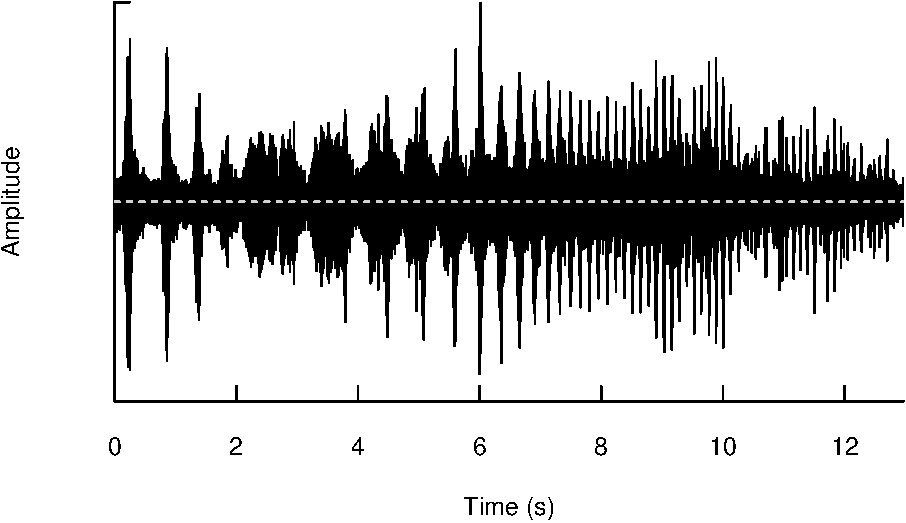
\includegraphics{behaviouR-R-package-tutorials_files/figure-latex/unnamed-chunk-58-1.pdf}

We can also zoom in so that we can actually see the shape of the wave.

\begin{Shaded}
\begin{Highlighting}[]
\NormalTok{seewave}\OperatorTok{::}\KeywordTok{oscillo}\NormalTok{(GibbonWaveFile, }\DataTypeTok{from=}\FloatTok{0.1}\NormalTok{, }\DataTypeTok{to=}\FloatTok{0.2}\NormalTok{)}
\end{Highlighting}
\end{Shaded}

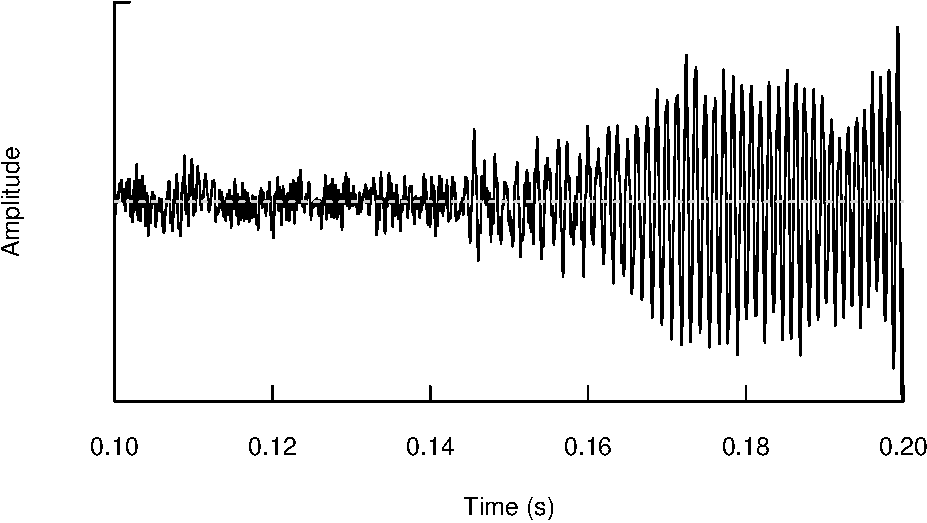
\includegraphics{behaviouR-R-package-tutorials_files/figure-latex/unnamed-chunk-59-1.pdf}

And if we zoom in again we see the wave shape even more.

\begin{Shaded}
\begin{Highlighting}[]
\NormalTok{seewave}\OperatorTok{::}\KeywordTok{oscillo}\NormalTok{(GibbonWaveFile, }\DataTypeTok{from=}\FloatTok{0.15}\NormalTok{, }\DataTypeTok{to=}\FloatTok{0.2}\NormalTok{)}
\end{Highlighting}
\end{Shaded}

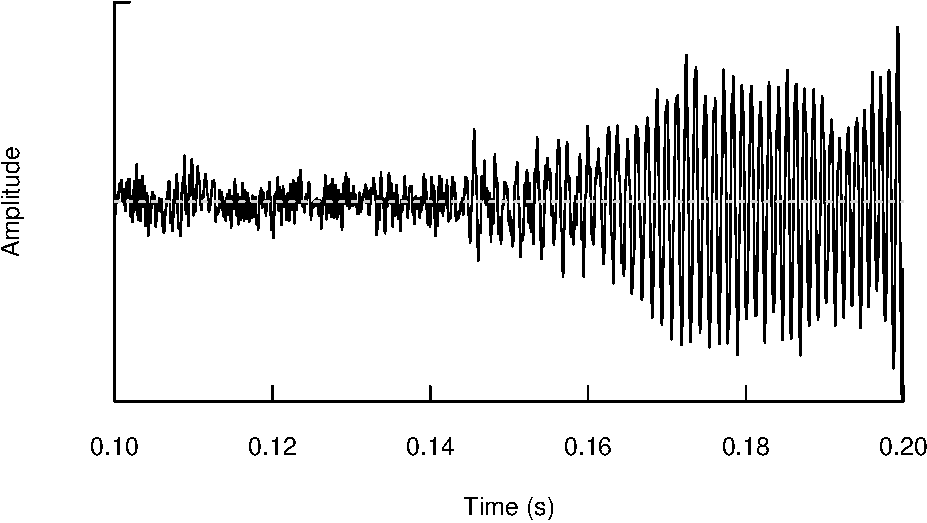
\includegraphics{behaviouR-R-package-tutorials_files/figure-latex/unnamed-chunk-60-1.pdf}

As we learned in class this week, a common way for scientists to study animal sounds is through the use of spectrograms. Here we will plot a spectrogram of a single gibbon call.

\begin{Shaded}
\begin{Highlighting}[]
\KeywordTok{SpectrogramSingle}\NormalTok{(}\DataTypeTok{sound.file =}\StringTok{"FocalRecordings/FemaleGibbon_1.wav"}\NormalTok{)}
\end{Highlighting}
\end{Shaded}

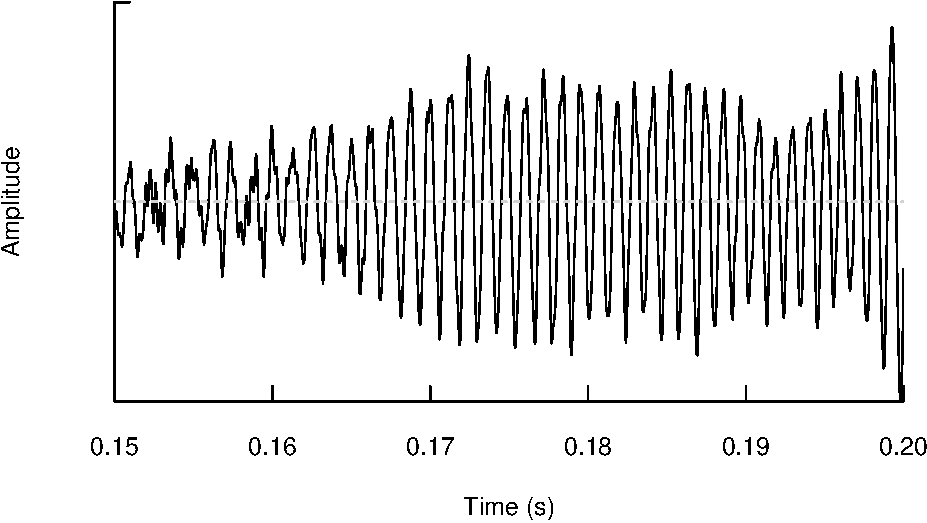
\includegraphics{behaviouR-R-package-tutorials_files/figure-latex/unnamed-chunk-61-1.pdf}

There are many different things you can change when creating a spectrogram. In the above version of the plot there is a lot of space above the gibbon calls, so we will change the frequency range to better visualize the gibbons.

\begin{Shaded}
\begin{Highlighting}[]
\KeywordTok{SpectrogramSingle}\NormalTok{(}\DataTypeTok{sound.file =}\StringTok{"FocalRecordings/FemaleGibbon_1.wav"}\NormalTok{,}
                  \DataTypeTok{min.freq =} \DecValTok{500}\NormalTok{,}\DataTypeTok{max.freq=}\DecValTok{2500}\NormalTok{)}
\end{Highlighting}
\end{Shaded}

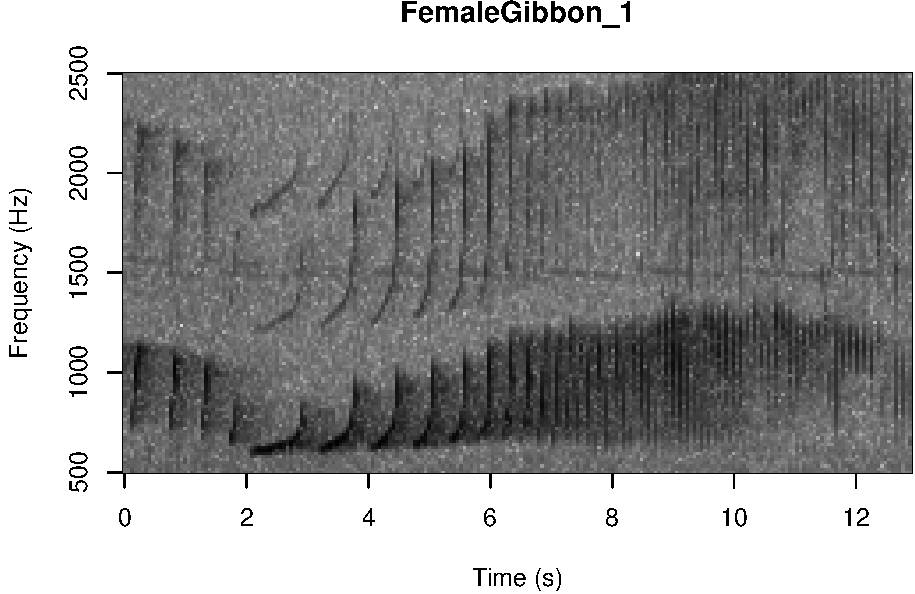
\includegraphics{behaviouR-R-package-tutorials_files/figure-latex/unnamed-chunk-62-1.pdf}

In the code we are using there is also the option to change the color of the spectrogram adding the following code:

\begin{Shaded}
\begin{Highlighting}[]
\KeywordTok{SpectrogramSingle}\NormalTok{(}\DataTypeTok{sound.file =}\StringTok{"FocalRecordings/FemaleGibbon_1.wav"}\NormalTok{,}
                  \DataTypeTok{min.freq =} \DecValTok{500}\NormalTok{,}\DataTypeTok{max.freq=}\DecValTok{2500}\NormalTok{,}
                  \DataTypeTok{Colors =} \StringTok{'Colors'}\NormalTok{)}
\end{Highlighting}
\end{Shaded}

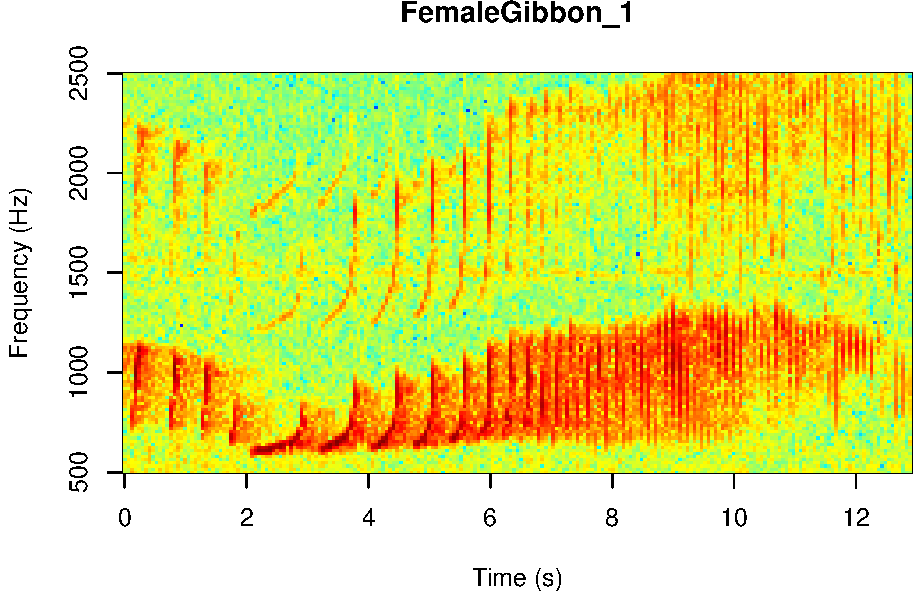
\includegraphics{behaviouR-R-package-tutorials_files/figure-latex/unnamed-chunk-63-1.pdf}

NOTE: Changing the colors doesn't change how we read the spectrograms,and different people have different preferences.

Now we can plot all of the spectrograms in our FocalRecordings file at once.

NOTE: Use the navigation buttons on the plots tab to move back and forth between the different spectrograms.

\begin{Shaded}
\begin{Highlighting}[]
\CommentTok{# We can tell R to print the spectrograms 2x2 using the code below}
\KeywordTok{par}\NormalTok{(}\DataTypeTok{mfrow=}\KeywordTok{c}\NormalTok{(}\DecValTok{2}\NormalTok{,}\DecValTok{2}\NormalTok{))}

\CommentTok{# This is the function to create the spectrograms}
  \KeywordTok{SpectrogramFunction}\NormalTok{(}\DataTypeTok{input.dir =} \StringTok{"FocalRecordings"}\NormalTok{,}\DataTypeTok{min.freq =} \DecValTok{500}\NormalTok{,}\DataTypeTok{max.freq=}\DecValTok{2500}\NormalTok{)}
\end{Highlighting}
\end{Shaded}

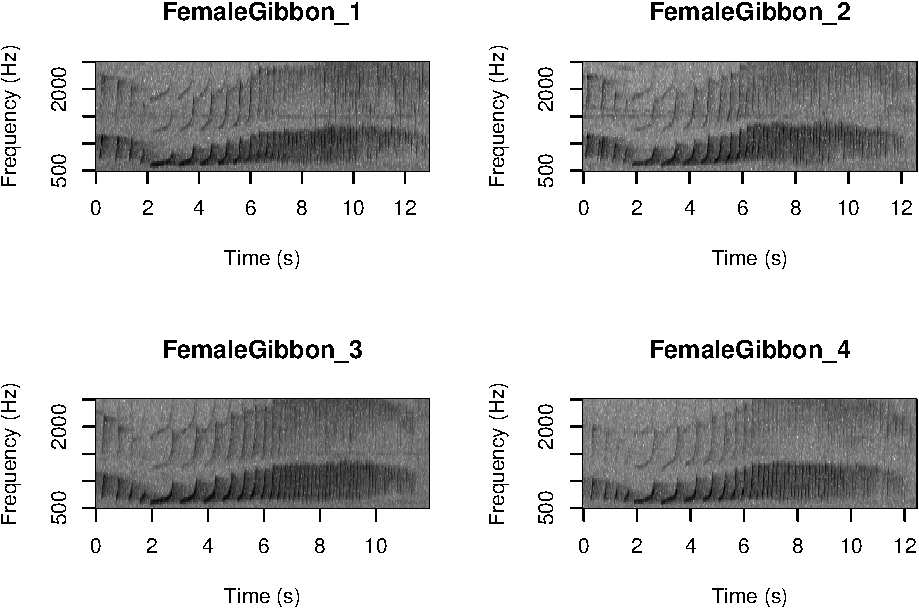
\includegraphics{behaviouR-R-package-tutorials_files/figure-latex/unnamed-chunk-64-1.pdf} 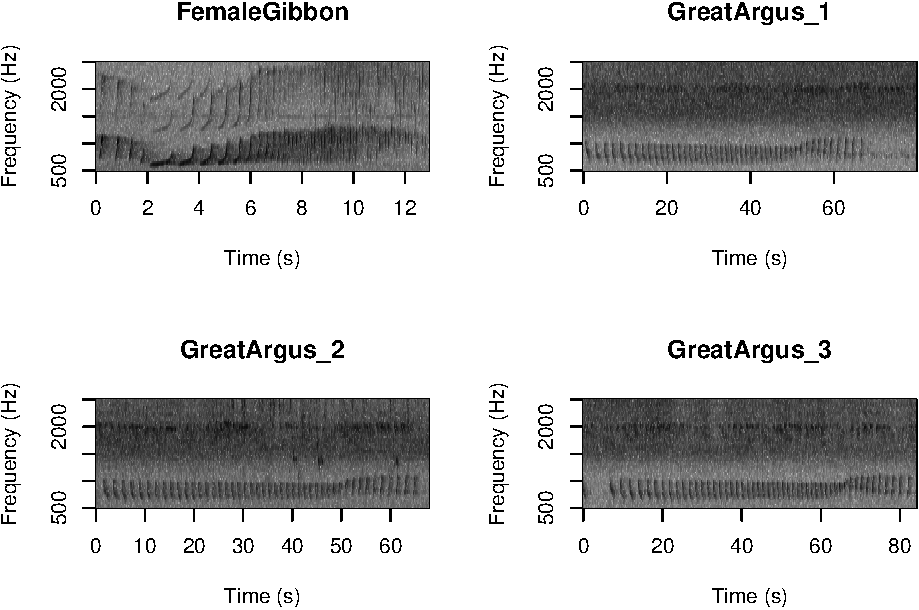
\includegraphics{behaviouR-R-package-tutorials_files/figure-latex/unnamed-chunk-64-2.pdf} 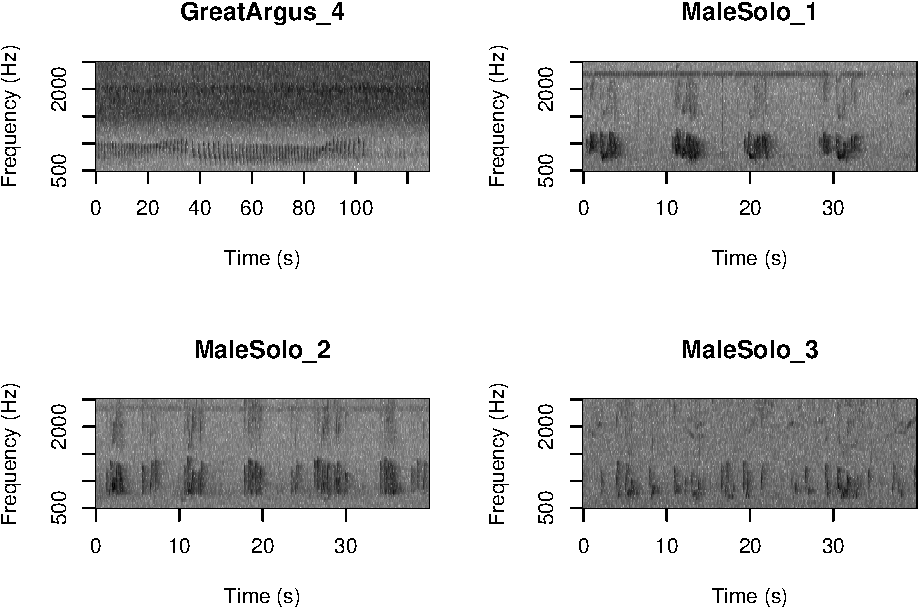
\includegraphics{behaviouR-R-package-tutorials_files/figure-latex/unnamed-chunk-64-3.pdf} 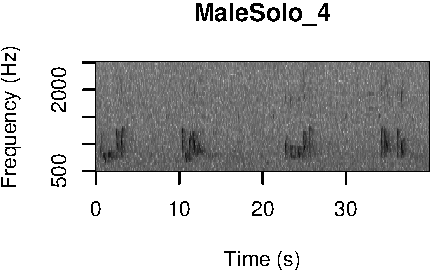
\includegraphics{behaviouR-R-package-tutorials_files/figure-latex/unnamed-chunk-64-4.pdf}

\emph{Question 1.} What differences do you notice about gibbon and great argus spectrograms?

Now that you are doing looking at the spectrograms we will clear the space. You can always re-run the code to look at the again.

\begin{Shaded}
\begin{Highlighting}[]
\KeywordTok{graphics.off}\NormalTok{()}
\end{Highlighting}
\end{Shaded}

\hypertarget{part-2.-visualizing-differences-in-gibbon-and-great-argus-calls}{%
\section*{Part 2. Visualizing differences in gibbon and great argus calls}\label{part-2.-visualizing-differences-in-gibbon-and-great-argus-calls}}
\addcontentsline{toc}{section}{Part 2. Visualizing differences in gibbon and great argus calls}

A major question in many different types of behavioral studies is whether there are differences between groups. This is also the case for acoustic data, where researchers may be interested if there are differences between sexes, populations, individuals, or vocalizations emitted in different contexts. Here we will work through a simple example where we will investigate differences in gibbon and argus calls.

The first step that we need to do is called feature extraction. There are many different ways that scientists do this, but the overarching idea is that sound data contains too much redundant information to be used on a model. Computers just don't have enough power to crunch all those numbers, so we need to identify a meaningful set of features that is smaller than using the while waveform. This is also the case for image processing.

We are going to use a feature extraction method called `Mel-frequency cepstral coefficients'. I will not expect you to know any more about them, apart from the fact they are very useful for human speech and bioaccoustics applications.

Below is the function to extract features from our focal recordings

\begin{Shaded}
\begin{Highlighting}[]
\NormalTok{FeatureDataframe <-}\StringTok{ }\KeywordTok{MFCCFunction}\NormalTok{(}\DataTypeTok{input.dir =} \StringTok{"FocalRecordings"}\NormalTok{)}
\end{Highlighting}
\end{Shaded}

In this new dataframe each row represents one gibbon or great argus call. Let's check the dimensions of this new dataframe.

\begin{Shaded}
\begin{Highlighting}[]
\KeywordTok{dim}\NormalTok{(FeatureDataframe)}
\end{Highlighting}
\end{Shaded}

\begin{verbatim}
## [1]  13 178
\end{verbatim}

This shows us that for each of the 10 calls there are 178 features. This is in contrast to a sound file. Let's check again to remind ourselves.

\begin{Shaded}
\begin{Highlighting}[]
\NormalTok{GibbonWaveFile}
\end{Highlighting}
\end{Shaded}

\begin{verbatim}
## 
## Wave Object
##  Number of Samples:      572054
##  Duration (seconds):     12.97
##  Samplingrate (Hertz):   44100
##  Channels (Mono/Stereo): Mono
##  PCM (integer format):   TRUE
##  Bit (8/16/24/32/64):    16
\end{verbatim}

This sound file is comprised of 572054 numbers. Now let's check the first row of our new dataframe which contains the new features for the same gibbon call.

\begin{Shaded}
\begin{Highlighting}[]
\CommentTok{# This isolates the first row.}
\NormalTok{FeatureDataframe[}\DecValTok{1}\NormalTok{,] }
\end{Highlighting}
\end{Shaded}

\begin{verbatim}
##          Class         1         2         3        4         5         6
## 1 FemaleGibbon -4.914312 -16.40678 -4.672827 20.59783 -4.632383 -6.999979
##          7         8        9       10        11        12        13        14
## 1 4.438287 -3.773641 -5.61846 10.73634 0.9757686 -1.163231 -6.800348 -17.70036
##          15       16       17       18       19        20        21        22
## 1 -2.564371 5.702963 8.604349 5.529339 2.561141 -2.507278 -8.423425 -6.229291
##          23        24        25        26      27       28       29       30
## 1 -3.115276 -7.588447 -23.27116 -3.826297 17.3082 8.632006 -1.60833 2.771364
##          31        32        33        34        35        36       37       38
## 1 -3.018685 -13.47489 -5.147027 -6.892077 -12.00958 -21.92954 9.776812 14.48623
##           39       40       41        42      43      44        45        46
## 1 0.08553639 2.275835 4.157477 -15.22412 -8.4252 8.55771 -7.545372 -20.37116
##          47       48        49       50       51        52        53       54
## 1 -9.496601 20.42913 0.1681313 2.009451 4.554415 -16.20235 -2.036649 9.715715
##          55        56       57        58       59        60       61       62
## 1 -1.521847 -4.390747 -23.6537 -1.739798 13.12778 -5.910114 6.569014 6.026896
##          63       64       65        66        67        68       69       70
## 1 -9.226613 -1.68419 4.550749 -5.170068 -10.94638 -20.08074 2.986301 9.424681
##          71       72      73        74         75       76       77        78
## 1 -6.254541 10.38071 -5.0744 -4.867023 -0.4075844 -2.65999 2.784278 -11.88797
##          79       80       81        82       83        84      85       86
## 1 -13.21431 5.279703 8.139582 -5.553872 5.027628 -3.739047 -3.1116 4.341732
##          87      88        89       90        91        92       93       94
## 1 -1.209793 1.00652 -1218.033 -1112.45 -830.5594 -462.4005 25.70725 66.06332
##          95        96       97       98       99       100      101      102
## 1 -5.735883 -36.24788 53.94479 37.60848 3.826036 -1222.493 -1046.01 -770.889
##         103      104      105     106       107       108       109       110
## 1 -393.6294 80.33639 49.16433 5.84342 -92.54861 -126.7318 -115.9133 -78.65571
##         111       112       113       114      115      116      117       118
## 1 -1222.167 -1044.567 -793.9816 -401.6897 87.24976 31.49047 -2.96363 -118.2727
##         119       120       121       122       123       124       125
## 1 -154.4816 -83.69734 -33.83878 -1229.136 -1086.172 -808.4772 -399.4776
##        126      127      128       129     130      131      132       133
## 1 53.89249 11.00474 11.99423 -57.18338 1.68353 85.31662 102.8748 -1239.725
##        134       135       136      137      138       139       140       141
## 1 -1088.64 -803.1513 -479.0124 44.22369 73.85069 -22.86258 -84.05236 -3.588271
##         142      143       144       145       146       147      148      149
## 1 -2.478177 9.528495 -1240.362 -1068.622 -782.7229 -440.9671 63.08211 80.21284
##         150       151       152    153       154       155       156       157
## 1 -46.79594 -82.71886 -40.87362 -75.92 -49.31079 -1285.428 -1091.577 -842.4694
##         158      159     160       161       162      163      164     165
## 1 -460.0004 72.63099 32.0981 -40.61593 -20.85975 31.29035 11.68475 66.2166
##         166       167       168       169     170      171       172       173
## 1 -1225.674 -1065.805 -823.5072 -452.4384 74.0775 24.51663 -33.48887 -13.24513
##        174      175      176      177
## 1 25.57118 3.053292 26.88251 12.97175
\end{verbatim}

\begin{Shaded}
\begin{Highlighting}[]
\CommentTok{# This tells us how many features we have.}
\KeywordTok{ncol}\NormalTok{(FeatureDataframe[}\DecValTok{1}\NormalTok{,]) }
\end{Highlighting}
\end{Shaded}

\begin{verbatim}
## [1] 178
\end{verbatim}

OK, now we are ready to do some plotting. If you remember from our earlier lab, the data structure we have here is multivariate, as each call has multiple values associated with it. So we will use the same approach (principal component analysis) to visualize our gibbon and great argus calls.

First we run the principal component analysis

\begin{Shaded}
\begin{Highlighting}[]
\NormalTok{pca_res <-}\StringTok{ }\KeywordTok{prcomp}\NormalTok{(FeatureDataframe[,}\OperatorTok{-}\KeywordTok{c}\NormalTok{(}\DecValTok{1}\NormalTok{)], }\DataTypeTok{scale. =} \OtherTok{TRUE}\NormalTok{)}
\end{Highlighting}
\end{Shaded}

Now we visualize our results

\begin{Shaded}
\begin{Highlighting}[]
\NormalTok{ggplot2}\OperatorTok{::}\KeywordTok{autoplot}\NormalTok{(pca_res, }\DataTypeTok{data =}\NormalTok{ FeatureDataframe, }
         \DataTypeTok{colour =} \StringTok{'Class'}\NormalTok{)}
\end{Highlighting}
\end{Shaded}

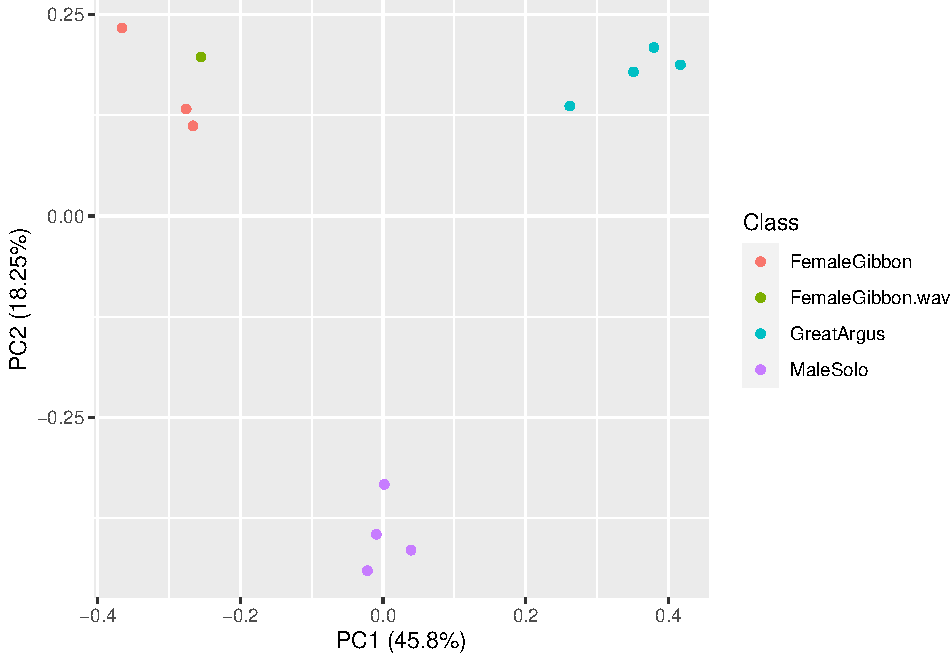
\includegraphics{behaviouR-R-package-tutorials_files/figure-latex/unnamed-chunk-71-1.pdf}

What we see in this plot is strong clustering, with the points from each class of calls more close to the other points than those of different calls.

\emph{Question 2.} How do we interpret the clustering in this PCA plot?

\hypertarget{part-3.-soundscapes}{%
\section*{Part 3. Soundscapes}\label{part-3.-soundscapes}}
\addcontentsline{toc}{section}{Part 3. Soundscapes}

Now we will do something similar to our investigation of the focal recordings, but using a soundscape example. Here we have 20-sec recordings taken from two different locations (Borneo and Sulawesi) and two different times (06:00 and 18:00). Let's check what is in the folder.

\begin{Shaded}
\begin{Highlighting}[]
\KeywordTok{list.files}\NormalTok{(}\StringTok{"SoundscapeRecordings"}\NormalTok{)}
\end{Highlighting}
\end{Shaded}

\begin{verbatim}
##  [1] "Borneo_Morning_01.wav"   "Borneo_Morning_02.wav"  
##  [3] "Borneo_Morning_03.wav"   "Borneo_Morning_04.wav"  
##  [5] "Borneo_Night_01.wav"     "Borneo_Night_02.wav"    
##  [7] "Borneo_Night_03.wav"     "Borneo_Night_04.wav"    
##  [9] "Sulawesi_Morning_01.wav" "Sulawesi_Morning_02.wav"
## [11] "Sulawesi_Morning_03.wav" "Sulawesi_Morning_04.wav"
## [13] "Sulawesi_Night_01.wav"   "Sulawesi_Night_02.wav"  
## [15] "Sulawesi_Night_03.wav"   "Sulawesi_Night_04.wav"
\end{verbatim}

Now we will create spectrograms for each recording

\begin{Shaded}
\begin{Highlighting}[]
\KeywordTok{par}\NormalTok{(}\DataTypeTok{mfrow=}\KeywordTok{c}\NormalTok{(}\DecValTok{2}\NormalTok{,}\DecValTok{2}\NormalTok{))}
\KeywordTok{SpectrogramFunctionSite}\NormalTok{(}\DataTypeTok{input.dir =} \StringTok{"SoundscapeRecordings"}\NormalTok{,}
                    \DataTypeTok{min.freq =} \DecValTok{0}\NormalTok{,}\DataTypeTok{max.freq=}\DecValTok{20000}\NormalTok{)}
\end{Highlighting}
\end{Shaded}

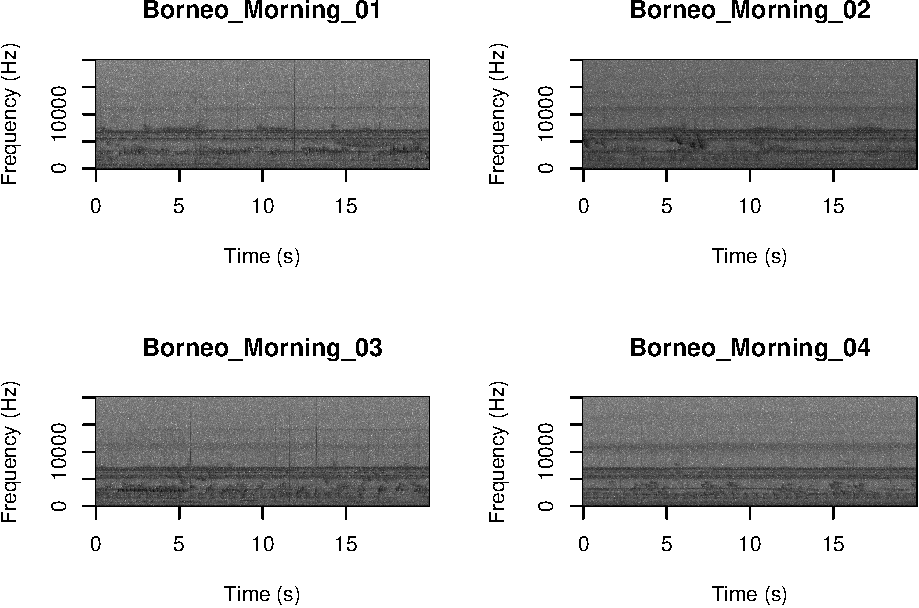
\includegraphics{behaviouR-R-package-tutorials_files/figure-latex/unnamed-chunk-73-1.pdf} 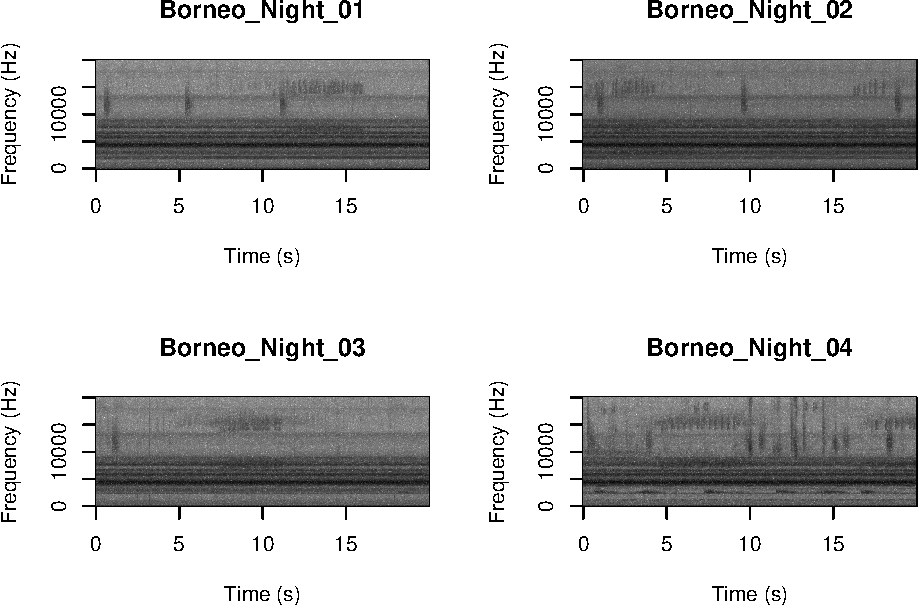
\includegraphics{behaviouR-R-package-tutorials_files/figure-latex/unnamed-chunk-73-2.pdf} 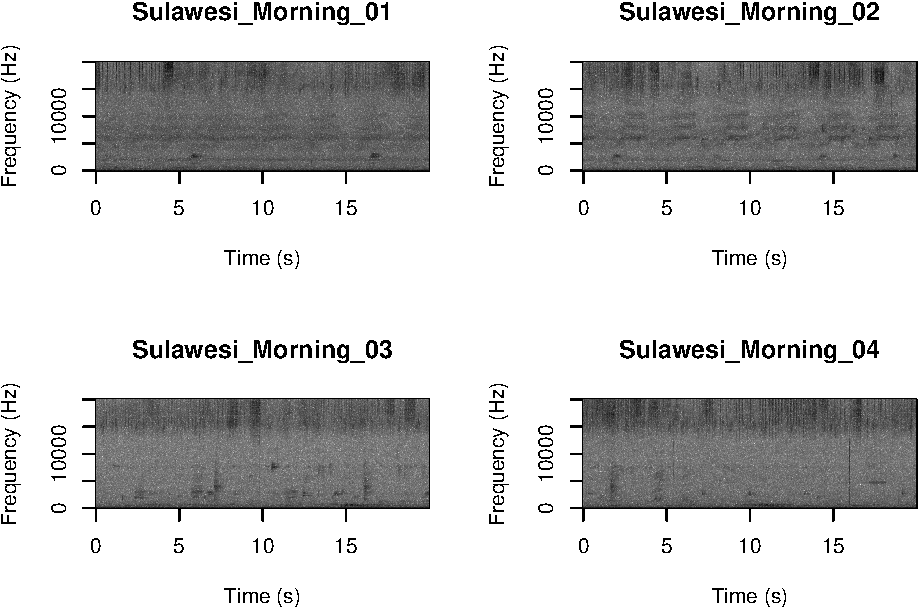
\includegraphics{behaviouR-R-package-tutorials_files/figure-latex/unnamed-chunk-73-3.pdf} 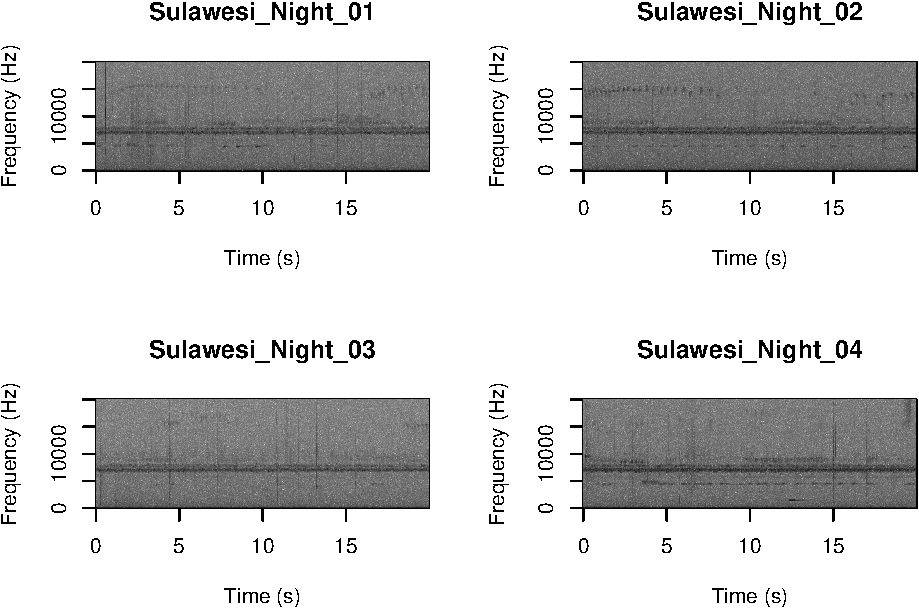
\includegraphics{behaviouR-R-package-tutorials_files/figure-latex/unnamed-chunk-73-4.pdf}

Now that you are doing looking at the figure we will clear the space. You can always re-run the code to look at the again.

\begin{Shaded}
\begin{Highlighting}[]
\KeywordTok{graphics.off}\NormalTok{()}
\end{Highlighting}
\end{Shaded}

Now just as above we will do feature extraction of our soundscape recordings. Thiswill convert our dataset into a smaller, much more manageable size.

\begin{Shaded}
\begin{Highlighting}[]
\NormalTok{SoundscapeFeatureDataframe <-}\StringTok{ }
\StringTok{  }\KeywordTok{MFCCFunctionSite}\NormalTok{(}\DataTypeTok{input.dir =} \StringTok{"SoundscapeRecordings"}\NormalTok{)}
\end{Highlighting}
\end{Shaded}

Check the resulting structure of the dataframe to make sure it looks OK.

\begin{Shaded}
\begin{Highlighting}[]
\KeywordTok{dim}\NormalTok{(SoundscapeFeatureDataframe)}
\end{Highlighting}
\end{Shaded}

\begin{verbatim}
## [1]  16 177
\end{verbatim}

Now we visualize our results

\begin{Shaded}
\begin{Highlighting}[]
\NormalTok{pca_res <-}\StringTok{ }\KeywordTok{prcomp}\NormalTok{(SoundscapeFeatureDataframe[,}\OperatorTok{-}\KeywordTok{c}\NormalTok{(}\DecValTok{1}\NormalTok{)], }\DataTypeTok{scale. =} \OtherTok{TRUE}\NormalTok{)}
\NormalTok{ggplot2}\OperatorTok{::}\KeywordTok{autoplot}\NormalTok{(pca_res, }\DataTypeTok{data =}\NormalTok{ SoundscapeFeatureDataframe, }
         \DataTypeTok{colour =} \StringTok{'Class'}\NormalTok{)}
\end{Highlighting}
\end{Shaded}

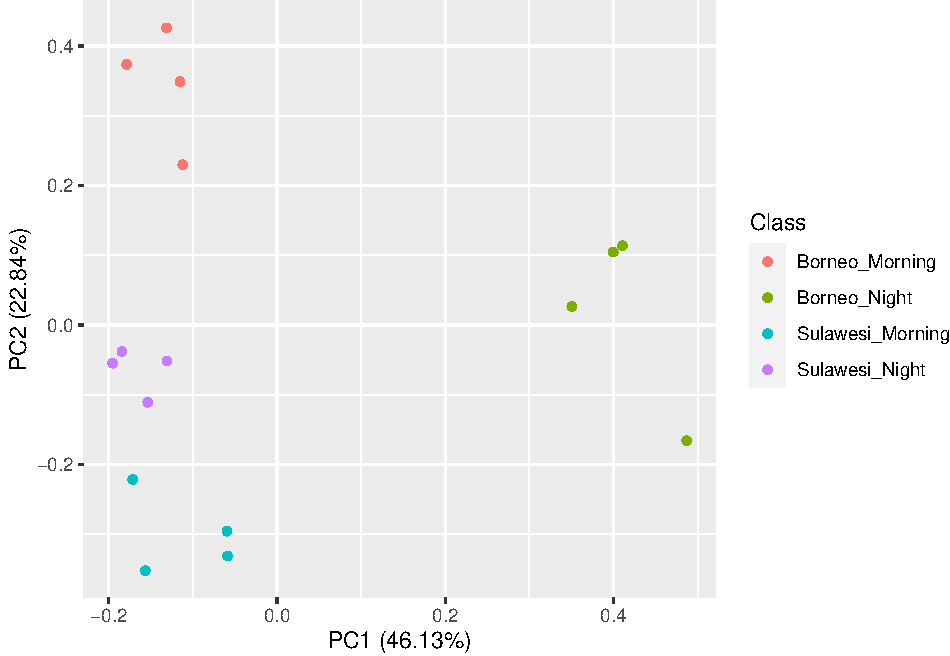
\includegraphics{behaviouR-R-package-tutorials_files/figure-latex/unnamed-chunk-77-1.pdf}

It looks like the Borneo\_Night sampling period was much different from the rest! Let's look at a single spectrogram from each sampling location and time.

\begin{Shaded}
\begin{Highlighting}[]
\KeywordTok{par}\NormalTok{(}\DataTypeTok{mfrow=}\KeywordTok{c}\NormalTok{(}\DecValTok{2}\NormalTok{,}\DecValTok{2}\NormalTok{))}
\KeywordTok{SpectrogramSingle}\NormalTok{(}\DataTypeTok{sound.file =}\StringTok{"SoundscapeRecordings/Borneo_Night_01.wav"}\NormalTok{,}
                  \DataTypeTok{min.freq =} \DecValTok{0}\NormalTok{,}\DataTypeTok{max.freq=}\DecValTok{22000}\NormalTok{,}
                  \DataTypeTok{Colors =} \StringTok{'Colors'}\NormalTok{,}\DataTypeTok{downsample =} \OtherTok{FALSE}\NormalTok{)}

\KeywordTok{SpectrogramSingle}\NormalTok{(}\DataTypeTok{sound.file =}\StringTok{"SoundscapeRecordings/Borneo_Morning_01.wav"}\NormalTok{,}
                  \DataTypeTok{min.freq =} \DecValTok{0}\NormalTok{,}\DataTypeTok{max.freq=}\DecValTok{22000}\NormalTok{,}
                  \DataTypeTok{Colors =} \StringTok{'Colors'}\NormalTok{,}\DataTypeTok{downsample =} \OtherTok{FALSE}\NormalTok{)}

\KeywordTok{SpectrogramSingle}\NormalTok{(}\DataTypeTok{sound.file =}\StringTok{"SoundscapeRecordings/Sulawesi_Night_01.wav"}\NormalTok{,}
                  \DataTypeTok{min.freq =} \DecValTok{0}\NormalTok{,}\DataTypeTok{max.freq=}\DecValTok{22000}\NormalTok{,}
                  \DataTypeTok{Colors =} \StringTok{'Colors'}\NormalTok{,}\DataTypeTok{downsample =} \OtherTok{FALSE}\NormalTok{)}

\KeywordTok{SpectrogramSingle}\NormalTok{(}\DataTypeTok{sound.file =}\StringTok{"SoundscapeRecordings/Sulawesi_Morning_01.wav"}\NormalTok{,}
                  \DataTypeTok{min.freq =} \DecValTok{0}\NormalTok{,}\DataTypeTok{max.freq=}\DecValTok{22000}\NormalTok{,}
                  \DataTypeTok{Colors =} \StringTok{'Colors'}\NormalTok{,}\DataTypeTok{downsample =} \OtherTok{FALSE}\NormalTok{)}
\end{Highlighting}
\end{Shaded}

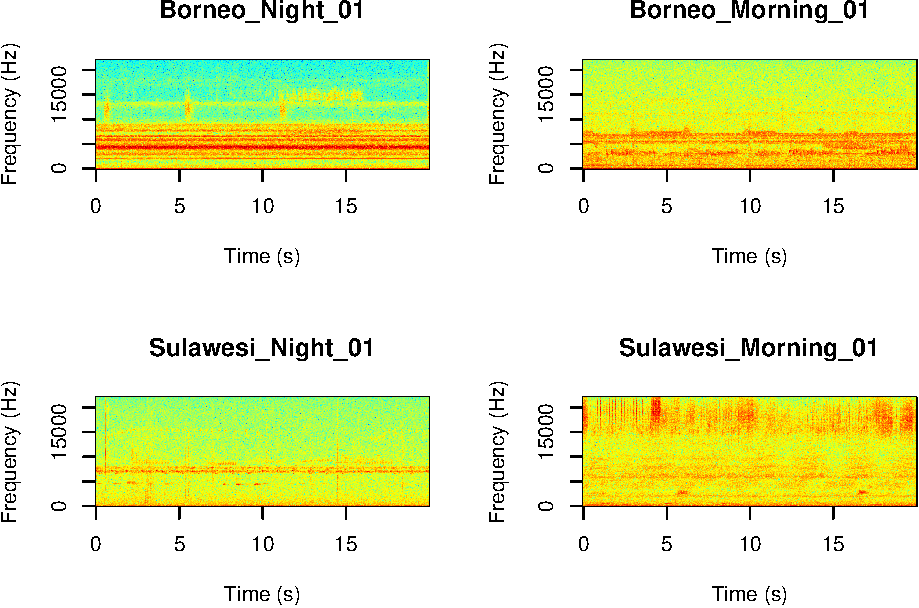
\includegraphics{behaviouR-R-package-tutorials_files/figure-latex/unnamed-chunk-78-1.pdf}

\emph{Question 3}. You can listen to example sound files on the Canvas page. Between looking at the spectrograms and listening to the sound files what do you think are the main differences between the different locations and times?

\hypertarget{part-4.-now-it-is-time-to-analyze-the-data-you-collected-for-this-weeks-field-lab.}{%
\section*{Part 4. Now it is time to analyze the data you collected for this week's field lab.}\label{part-4.-now-it-is-time-to-analyze-the-data-you-collected-for-this-weeks-field-lab.}}
\addcontentsline{toc}{section}{Part 4. Now it is time to analyze the data you collected for this week's field lab.}

Upload your sound files into either the `MyFocalRecordings' folder or the 'MySoundscapeRecordings'folder and run the code below.

NOTE: Make sure to delete the existing files before you add your own!

\hypertarget{part-4a.-your-focal-recordings}{%
\subsection{Part 4a. Your focal recordings}\label{part-4a.-your-focal-recordings}}

First lets visualize the spectrograms. You may want to change the frequency settings depending on the frequency range of your focal animals.

\begin{Shaded}
\begin{Highlighting}[]
\CommentTok{# We can tell R to print the spectrograms 2x2 using the code below}
\KeywordTok{par}\NormalTok{(}\DataTypeTok{mfrow=}\KeywordTok{c}\NormalTok{(}\DecValTok{2}\NormalTok{,}\DecValTok{2}\NormalTok{))}

\CommentTok{# This is the function to create the spectrograms}
\KeywordTok{SpectrogramFunction}\NormalTok{(}\DataTypeTok{input.dir =} \StringTok{"MyFocalRecordings"}\NormalTok{,}\DataTypeTok{min.freq =} \DecValTok{200}\NormalTok{,}\DataTypeTok{max.freq=}\DecValTok{2000}\NormalTok{)}
\end{Highlighting}
\end{Shaded}

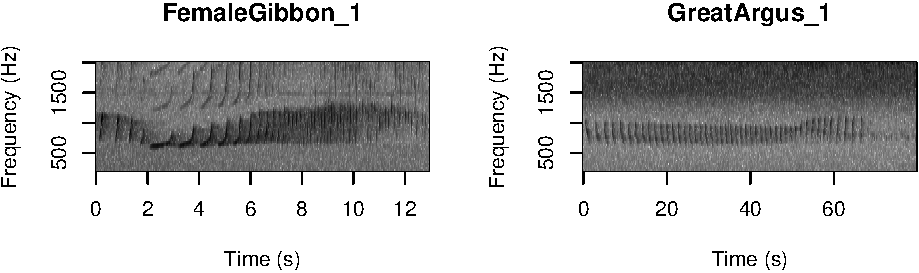
\includegraphics{behaviouR-R-package-tutorials_files/figure-latex/unnamed-chunk-79-1.pdf}

Here is the function to extract the features. Again, based on the frequency range of your focal recordings you may want to change the frequency settings.

\begin{Shaded}
\begin{Highlighting}[]
\NormalTok{MyFeatureDataFrame <-}\StringTok{ }\KeywordTok{MFCCFunction}\NormalTok{(}\DataTypeTok{input.dir =} \StringTok{"MyFocalRecordings"}\NormalTok{,}\DataTypeTok{min.freq =} \DecValTok{200}\NormalTok{,}\DataTypeTok{max.freq=}\DecValTok{2000}\NormalTok{)}
\end{Highlighting}
\end{Shaded}

Then we run the principal component analysis

\begin{Shaded}
\begin{Highlighting}[]
\NormalTok{pca_res <-}\StringTok{ }\KeywordTok{prcomp}\NormalTok{(MyFeatureDataFrame[,}\OperatorTok{-}\KeywordTok{c}\NormalTok{(}\DecValTok{1}\NormalTok{)], }\DataTypeTok{scale. =} \OtherTok{TRUE}\NormalTok{)}
\end{Highlighting}
\end{Shaded}

Now we visualize our results

\begin{Shaded}
\begin{Highlighting}[]
\NormalTok{ggplot2}\OperatorTok{::}\KeywordTok{autoplot}\NormalTok{(pca_res, }\DataTypeTok{data =}\NormalTok{ MyFeatureDataFrame,}
         \DataTypeTok{colour =} \StringTok{'Class'}\NormalTok{)}
\end{Highlighting}
\end{Shaded}

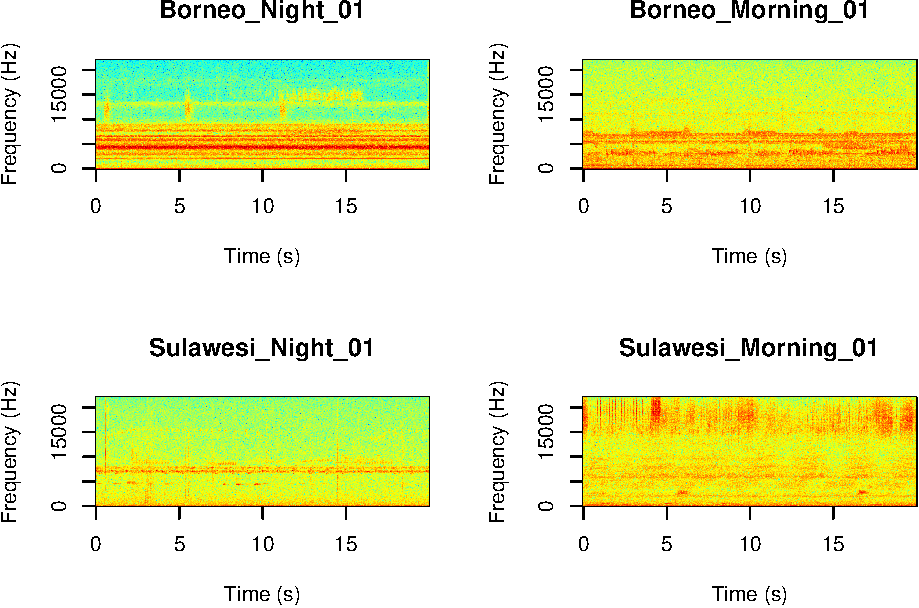
\includegraphics{behaviouR-R-package-tutorials_files/figure-latex/unnamed-chunk-82-1.pdf}

\hypertarget{part-4b.-soundscape-recordings}{%
\subsection{Part 4b. Soundscape recordings}\label{part-4b.-soundscape-recordings}}

First lets visualize the spectrograms. You probably don't want to change the frequency settings for this.

\begin{Shaded}
\begin{Highlighting}[]
\CommentTok{# We can tell R to print the spectrograms 2x2 using the code below}
\KeywordTok{par}\NormalTok{(}\DataTypeTok{mfrow=}\KeywordTok{c}\NormalTok{(}\DecValTok{2}\NormalTok{,}\DecValTok{2}\NormalTok{))}

\CommentTok{# This is the function to create the spectrograms}
\KeywordTok{SpectrogramFunction}\NormalTok{(}\DataTypeTok{input.dir =} \StringTok{"MySoundscapeRecordings"}\NormalTok{,}\DataTypeTok{min.freq =} \DecValTok{200}\NormalTok{,}\DataTypeTok{max.freq=}\DecValTok{10000}\NormalTok{)}
\end{Highlighting}
\end{Shaded}

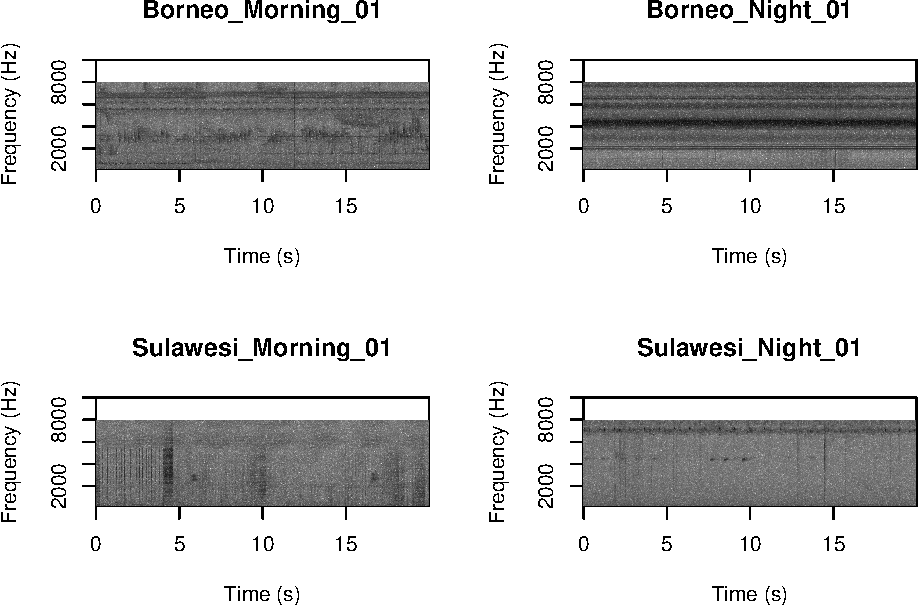
\includegraphics{behaviouR-R-package-tutorials_files/figure-latex/unnamed-chunk-83-1.pdf}

Then we extract the features, which in this case are the MFCCs.

\begin{Shaded}
\begin{Highlighting}[]
\NormalTok{MySoundscapeFeatureDataframe <-}\StringTok{ }
\StringTok{  }\KeywordTok{MFCCFunctionSite}\NormalTok{(}\DataTypeTok{input.dir =} \StringTok{"MySoundscapeRecordings"}\NormalTok{,}\DataTypeTok{min.freq =} \DecValTok{200}\NormalTok{,}\DataTypeTok{max.freq=}\DecValTok{10000}\NormalTok{)}
\end{Highlighting}
\end{Shaded}

Check the resulting structure of the dataframe to make sure it looks OK.

\begin{Shaded}
\begin{Highlighting}[]
\KeywordTok{dim}\NormalTok{(MySoundscapeFeatureDataframe)}
\end{Highlighting}
\end{Shaded}

Now we visualize our results

\begin{Shaded}
\begin{Highlighting}[]
\NormalTok{pca_res <-}\StringTok{ }\KeywordTok{prcomp}\NormalTok{(MySoundscapeFeatureDataframe[,}\OperatorTok{-}\KeywordTok{c}\NormalTok{(}\DecValTok{1}\NormalTok{)], }\DataTypeTok{scale. =} \OtherTok{TRUE}\NormalTok{)}
\NormalTok{ggplot2}\OperatorTok{::}\KeywordTok{autoplot}\NormalTok{(pca_res, }\DataTypeTok{data =}\NormalTok{ MySoundscapeFeatureDataframe, }
         \DataTypeTok{colour =} \StringTok{'Class'}\NormalTok{)}
\end{Highlighting}
\end{Shaded}

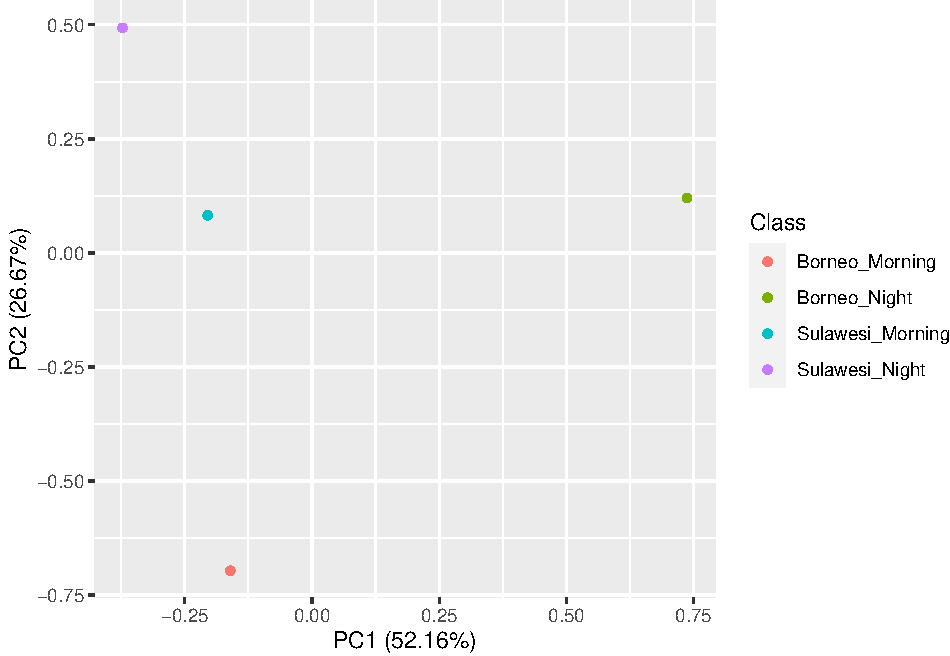
\includegraphics{behaviouR-R-package-tutorials_files/figure-latex/unnamed-chunk-86-1.pdf}

\emph{Question 4}. Do you see evidence of clustering in either your focal recordings or soundscape recordings?

\hypertarget{computer-lab-4.-vigilance-behavior}{%
\chapter*{Computer Lab 4. Vigilance behavior}\label{computer-lab-4.-vigilance-behavior}}
\addcontentsline{toc}{chapter}{Computer Lab 4. Vigilance behavior}

\begin{center}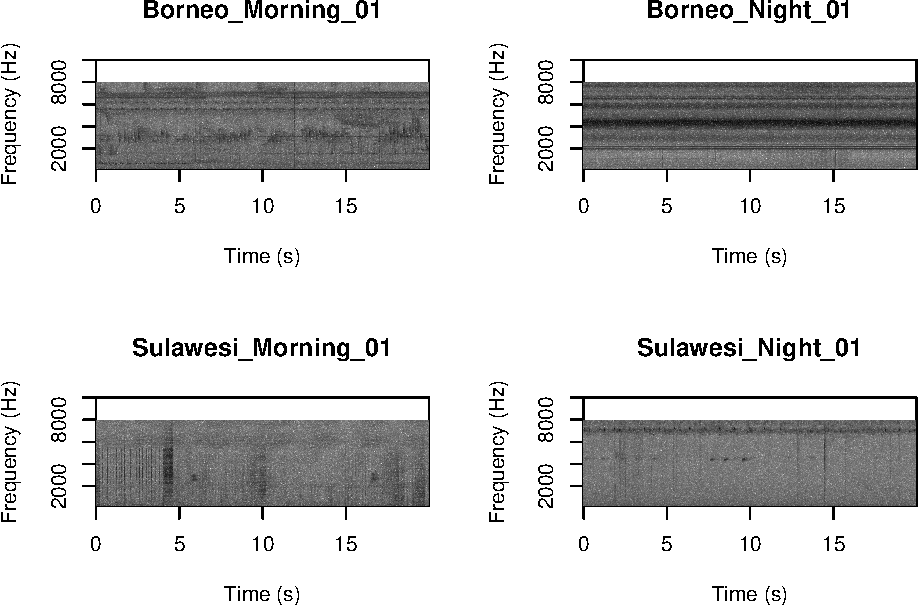
\includegraphics{behaviouR-R-package-tutorials_files/figure-latex/unnamed-chunk-87-1} \end{center}

\emph{Background}\\
In this lab we will continue our work investigating vigilance behaviors in geese and meerkats.

\emph{Goals of the exercises}\\
The main goal(s) of today's lab are to:\\
1) Use the data on goose vigilance behavior to investigate the relationship between group size and vigilance behaviors.\\
2) Analyze the data collected during the meerkat lab to test for differences in vigilant behavior across predator treatment groups.\\
3) Continue to become familar with the way scientists analyze and interpret data.

\emph{Getting started}\\
First we need to load the relevant packages for our data analysis. Packages contain all the functions that are needed for data analysis.
First we load the required libraries

\begin{Shaded}
\begin{Highlighting}[]
\KeywordTok{library}\NormalTok{(behaviouR)}
\KeywordTok{library}\NormalTok{(ggpubr)}
\end{Highlighting}
\end{Shaded}

\hypertarget{part-1-barnacle-goose-vigilance}{%
\section*{Part 1: Barnacle goose vigilance}\label{part-1-barnacle-goose-vigilance}}
\addcontentsline{toc}{section}{Part 1: Barnacle goose vigilance}

First, load the goose data that you collected using the following code.

\begin{Shaded}
\begin{Highlighting}[]
\NormalTok{BarnacleGooseData <-}\StringTok{ }\KeywordTok{read.csv}\NormalTok{(}\StringTok{'BarnacleGooseData.csv'}\NormalTok{)}
\end{Highlighting}
\end{Shaded}

Or you can use the data that comes with the package.

\begin{Shaded}
\begin{Highlighting}[]
\KeywordTok{data}\NormalTok{(}\StringTok{"BarnacleGooseData"}\NormalTok{)}
\end{Highlighting}
\end{Shaded}

\hypertarget{part-1a-surveillance-behavior}{%
\subsection*{Part 1a: Surveillance behavior}\label{part-1a-surveillance-behavior}}
\addcontentsline{toc}{subsection}{Part 1a: Surveillance behavior}

First, we will calculate the surveillance rate (or the number of heads up per minute). Let's start by looking at the total number of `head up' behaviors in our data. To investigate this relationship we will create a scatterplot.

\begin{Shaded}
\begin{Highlighting}[]
\CommentTok{# Scatterplot of total number of 'head up' in our data}
\KeywordTok{ggscatter}\NormalTok{(}\DataTypeTok{data=}\NormalTok{BarnacleGooseData,}
          \DataTypeTok{x=}\StringTok{'FlockSize'}\NormalTok{,}\DataTypeTok{y=}\StringTok{'TotalHeadsUp'}\NormalTok{)}\OperatorTok{+}\KeywordTok{ylab}\NormalTok{(}\StringTok{'Surveillance rate'}\NormalTok{)}
\end{Highlighting}
\end{Shaded}

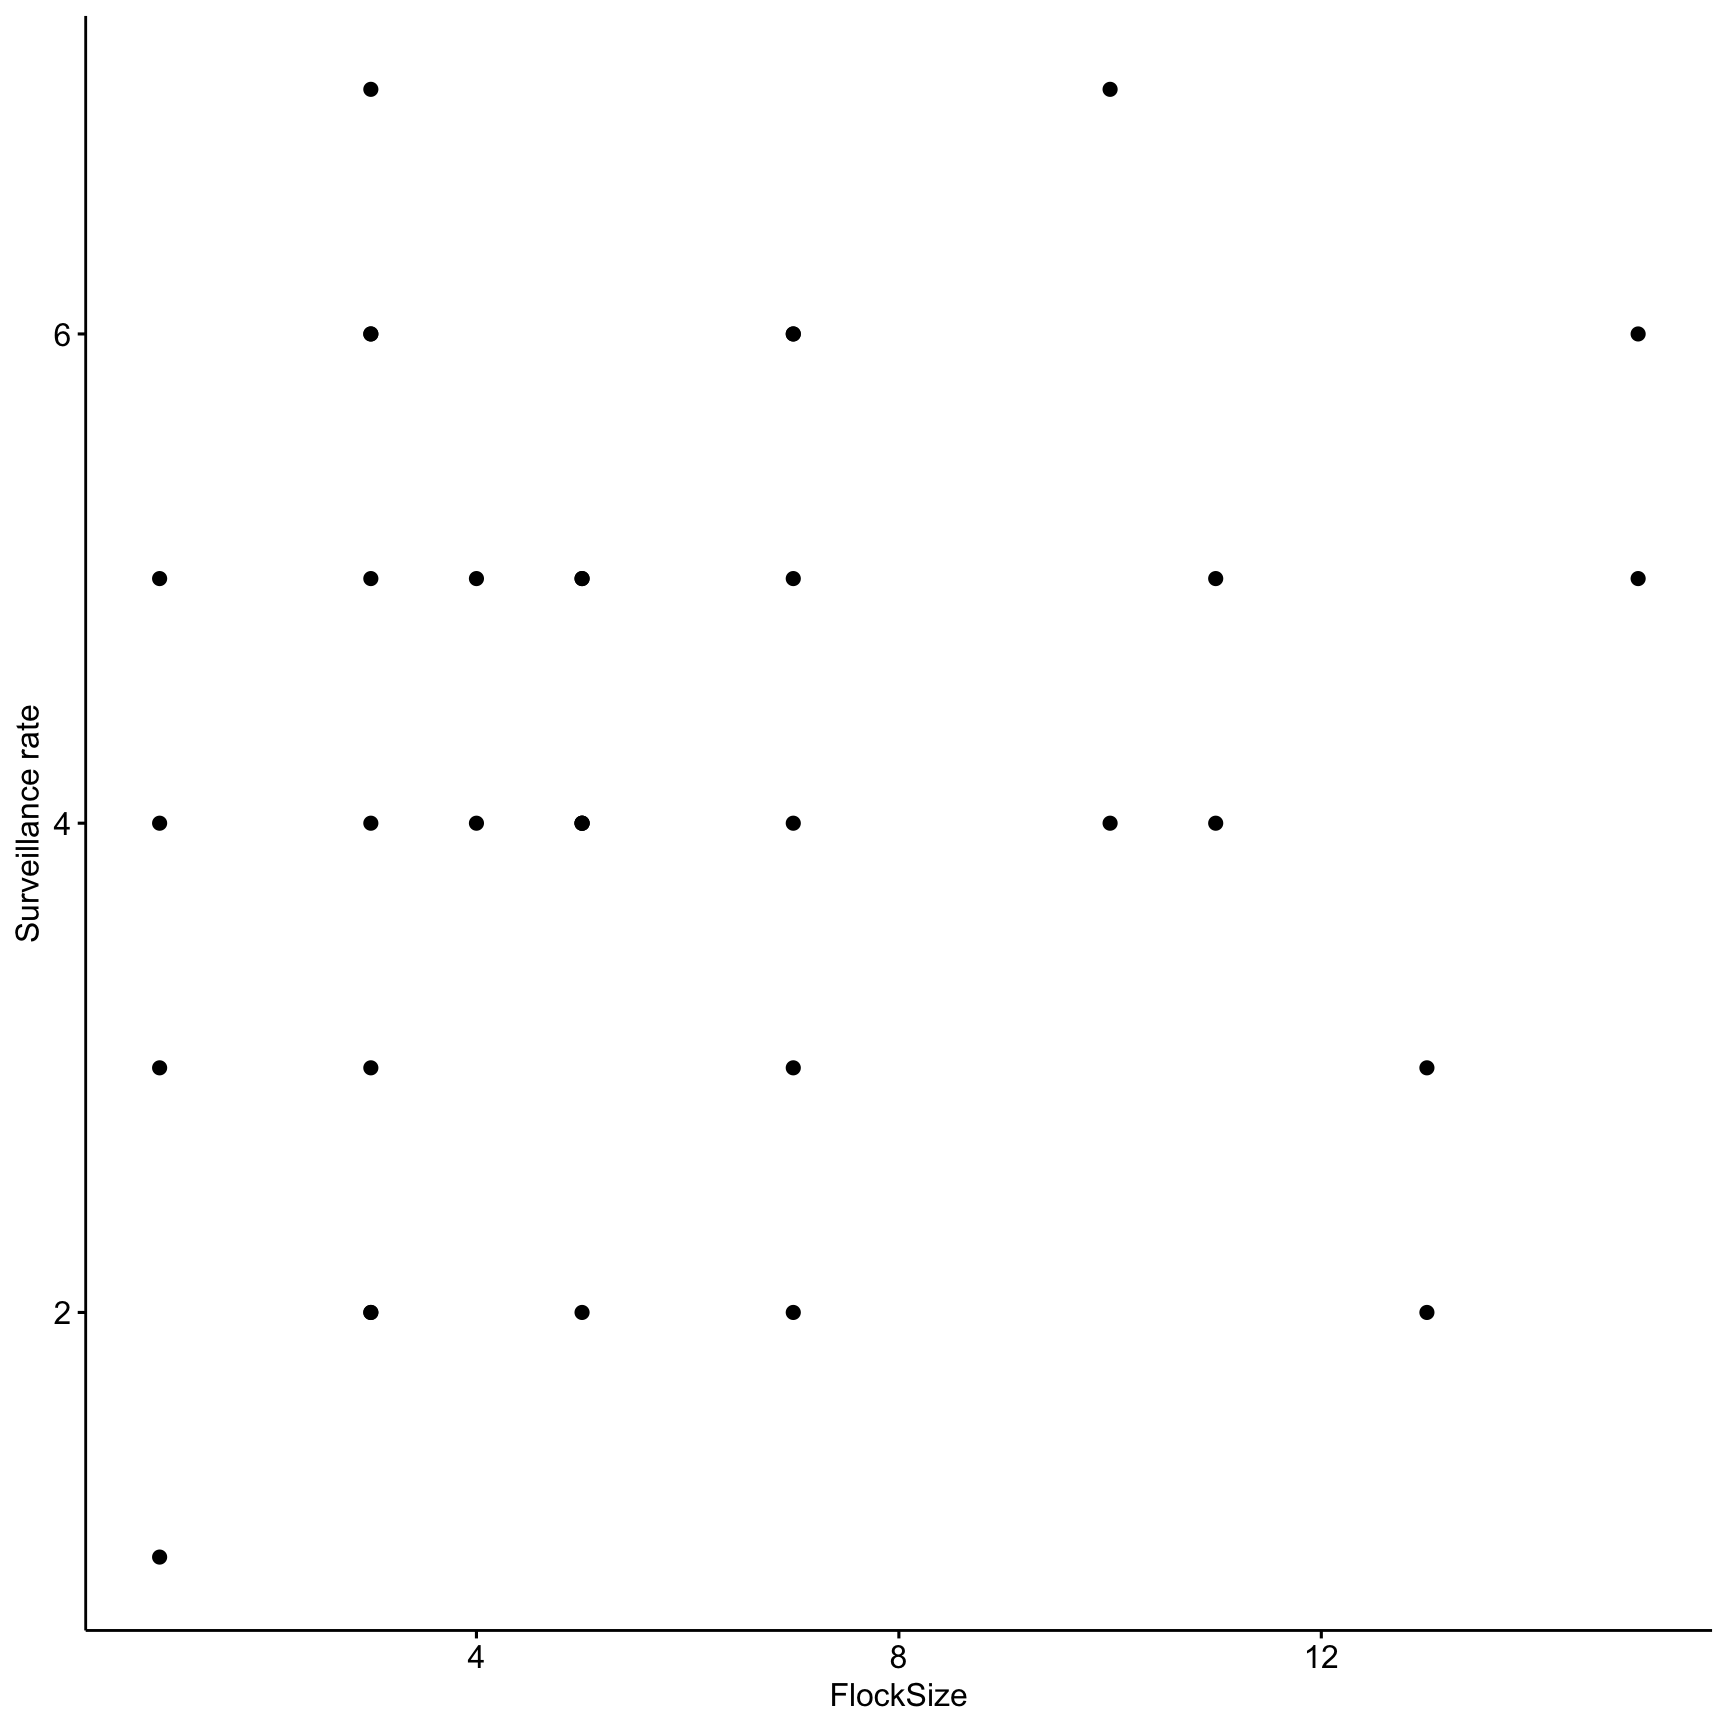
\includegraphics{behaviouR-R-package-tutorials_files/figure-latex/unnamed-chunk-91-1.pdf}

Now let's add a trend line to see if there is a relationship between flock size and the total number of `head up' behaviors

\begin{Shaded}
\begin{Highlighting}[]
\CommentTok{# Scatterplot of total number of 'head up' in our data with a trend line.}

\KeywordTok{ggscatter}\NormalTok{(}\DataTypeTok{data=}\NormalTok{BarnacleGooseData,}
          \DataTypeTok{x=}\StringTok{'FlockSize'}\NormalTok{,}\DataTypeTok{y=}\StringTok{'TotalHeadsUp'}\NormalTok{,}\DataTypeTok{add=}\StringTok{'reg.line'}\NormalTok{)}\OperatorTok{+}\KeywordTok{ylab}\NormalTok{(}\StringTok{'Surveillance rate'}\NormalTok{)}
\end{Highlighting}
\end{Shaded}

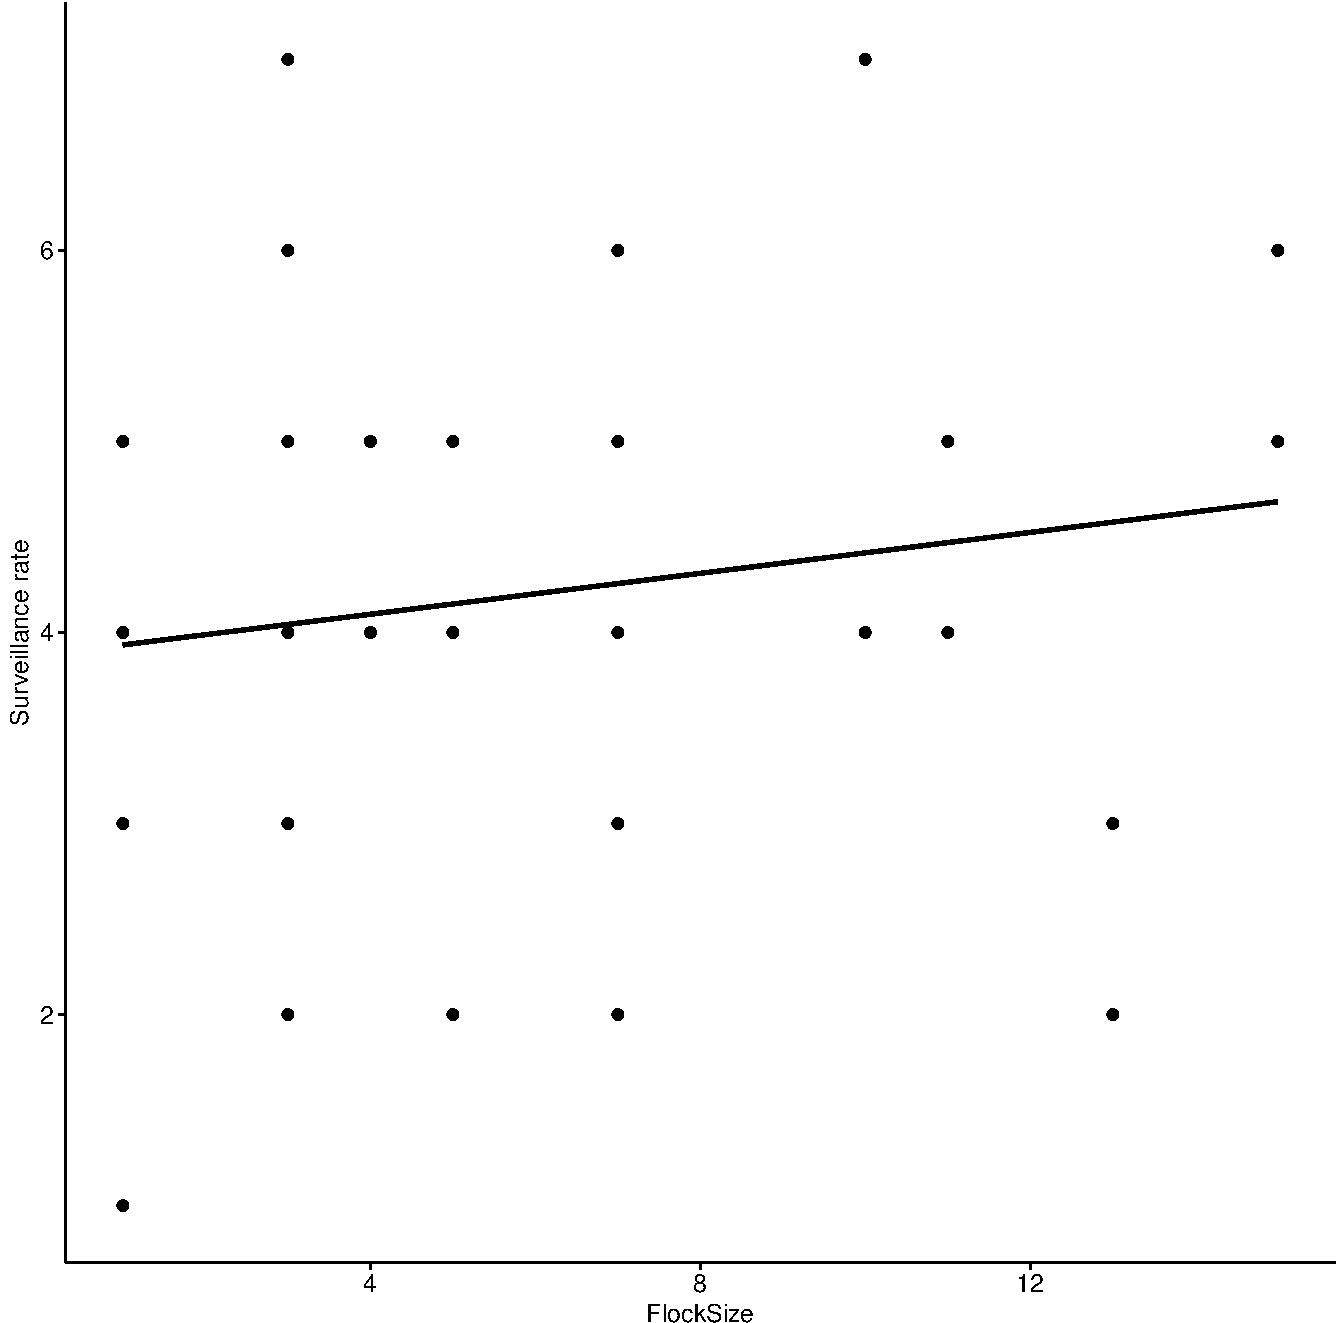
\includegraphics{behaviouR-R-package-tutorials_files/figure-latex/unnamed-chunk-92-1.pdf}

Let's see if there were any differences between you and your partner. We will also add the command `cor.coef = T' which will give us the correlation coefficient (R) along with an associated p-value.

\begin{Shaded}
\begin{Highlighting}[]
\CommentTok{# }\AlertTok{NOTE}\CommentTok{: The data here are simulated so your plots should look different}
\KeywordTok{ggscatter}\NormalTok{(}\DataTypeTok{data=}\NormalTok{BarnacleGooseData,}
          \DataTypeTok{x=}\StringTok{'FlockSize'}\NormalTok{,}\DataTypeTok{y=}\StringTok{'TotalHeadsUp'}\NormalTok{,}\DataTypeTok{add=}\StringTok{'reg.line'}\NormalTok{, }\DataTypeTok{facet.by =} \StringTok{'Partner'}\NormalTok{,}
          \DataTypeTok{cor.coef =}\NormalTok{ T)}\OperatorTok{+}\KeywordTok{ylab}\NormalTok{(}\StringTok{'Surveillance rate'}\NormalTok{)}
\end{Highlighting}
\end{Shaded}

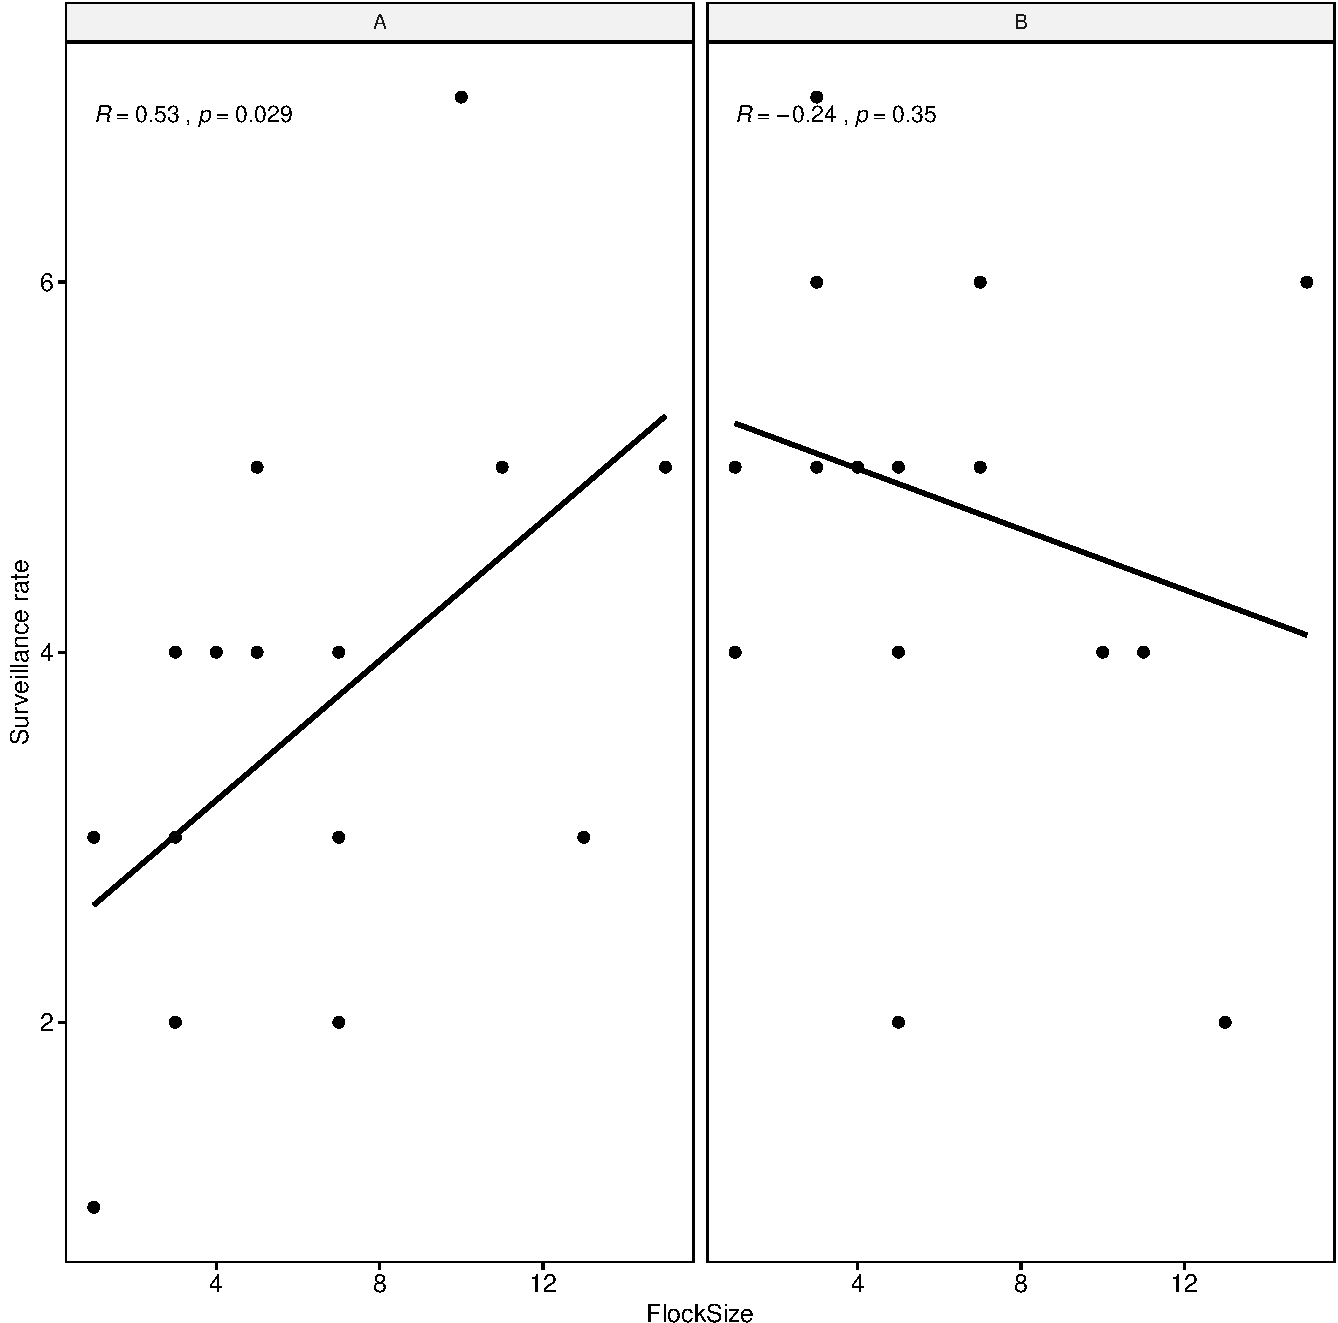
\includegraphics{behaviouR-R-package-tutorials_files/figure-latex/unnamed-chunk-93-1.pdf}

Let's plot you and your partner's data in different colors.

\begin{Shaded}
\begin{Highlighting}[]
\KeywordTok{ggscatter}\NormalTok{(}\DataTypeTok{data=}\NormalTok{BarnacleGooseData,}
          \DataTypeTok{x=}\StringTok{'FlockSize'}\NormalTok{,}\DataTypeTok{y=}\StringTok{'TotalHeadsUp'}\NormalTok{,}\DataTypeTok{add=}\StringTok{'reg.line'}\NormalTok{, }\DataTypeTok{facet.by =} \StringTok{'Partner'}\NormalTok{,}
          \DataTypeTok{color =} \StringTok{'Partner'}\NormalTok{, }\DataTypeTok{palette =}\KeywordTok{c}\NormalTok{(}\StringTok{'black'}\NormalTok{,}\StringTok{'blue'}\NormalTok{),}
          \DataTypeTok{cor.coef =}\NormalTok{ T)}\OperatorTok{+}\KeywordTok{ylab}\NormalTok{(}\StringTok{'Surveillance rate'}\NormalTok{)}
\end{Highlighting}
\end{Shaded}

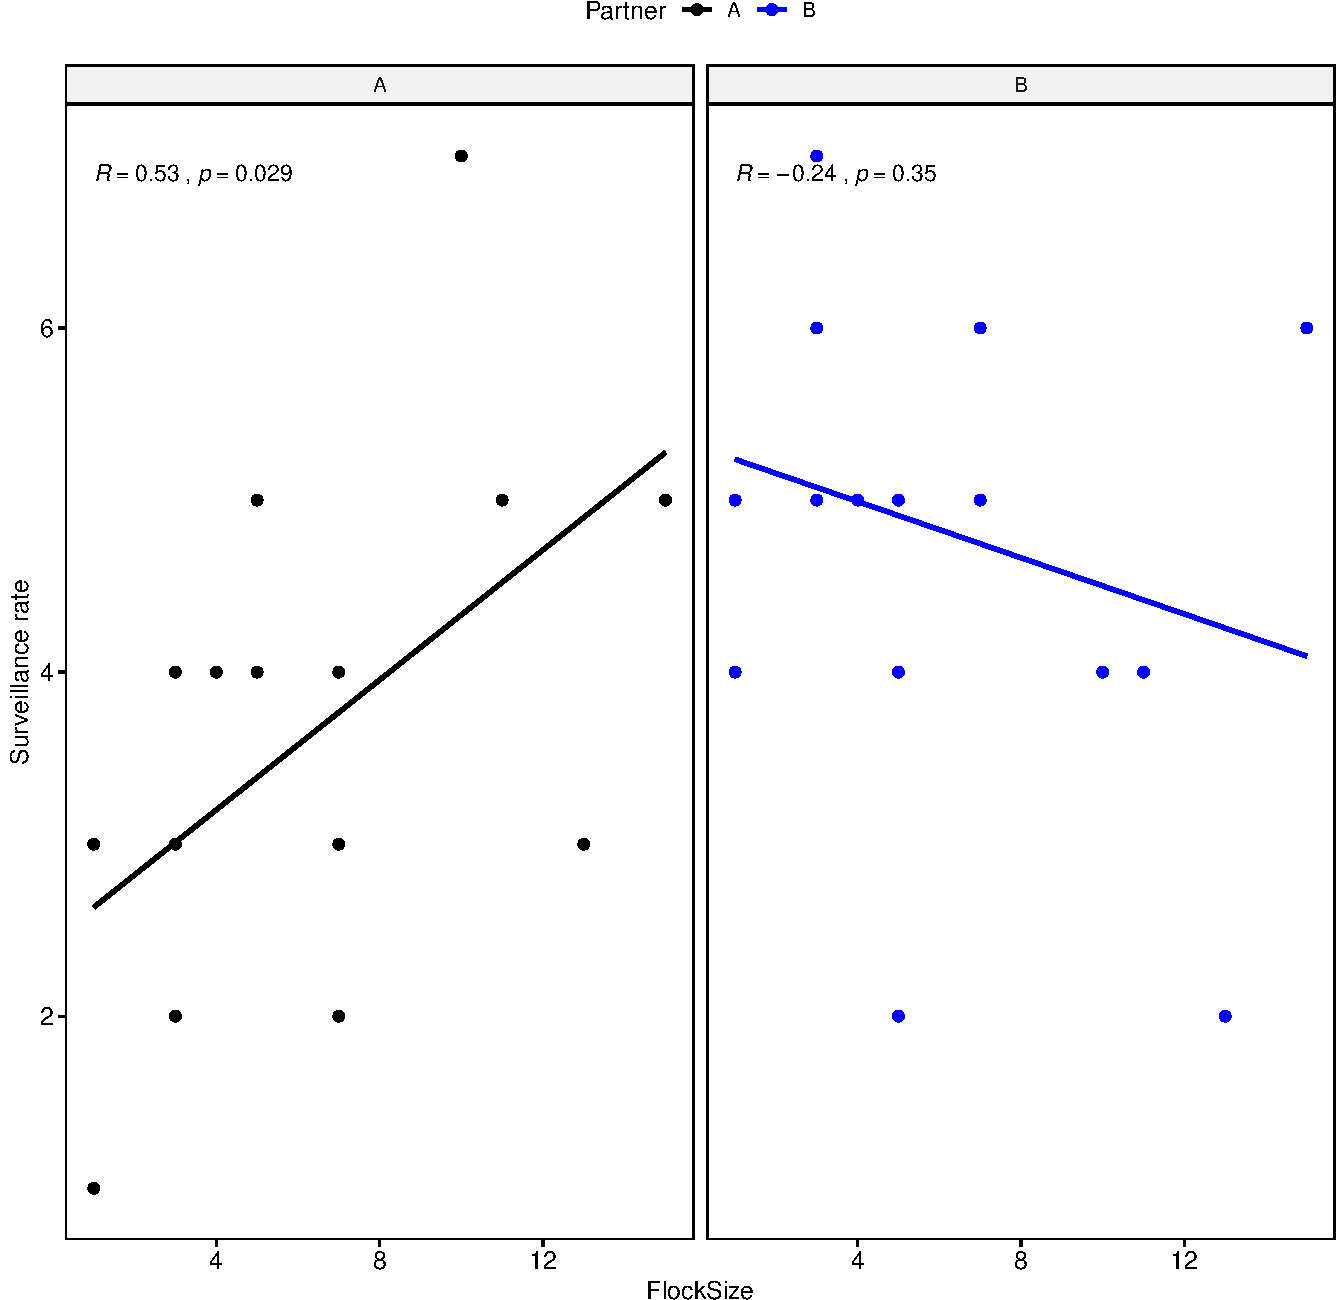
\includegraphics{behaviouR-R-package-tutorials_files/figure-latex/unnamed-chunk-94-1.pdf}

\textbf{Question 1}: Were there any major differences between you and your partner in terms of the observed relationship between flock size and surveillance rate?

Now we will do model selection using Akaike information criterion (AIC). First we create a null model and then we create a model with flock size as a predictor of total number of heads up. In the model code we specify that we are using a Poisson distribution, as we are dealing with count data instead of a continuous variable.

\begin{Shaded}
\begin{Highlighting}[]
\CommentTok{# This is our null model}
\NormalTok{SurveillanceNullModel <-}\StringTok{ }\KeywordTok{glm}\NormalTok{(TotalHeadsUp }\OperatorTok{~}\StringTok{ }\NormalTok{(}\DecValTok{1}\OperatorTok{/}\NormalTok{Partner),}\DataTypeTok{family=}\NormalTok{poisson , }\DataTypeTok{data=}\NormalTok{BarnacleGooseData)}

\CommentTok{# This is our model with flock size as a predictor of total number of heads up}
\NormalTok{SurveillanceModel <-}\StringTok{ }\KeywordTok{glm}\NormalTok{(TotalHeadsUp }\OperatorTok{~}\StringTok{ }\NormalTok{FlockSize }\OperatorTok{+}\StringTok{ }\NormalTok{(}\DecValTok{1}\OperatorTok{/}\NormalTok{Partner) ,}\DataTypeTok{family=}\NormalTok{poisson, }\DataTypeTok{data=}\NormalTok{BarnacleGooseData)}

\CommentTok{# Then we compare the models using AIC}
\NormalTok{bbmle}\OperatorTok{::}\KeywordTok{AICtab}\NormalTok{(SurveillanceNullModel,SurveillanceModel)}
\end{Highlighting}
\end{Shaded}

\begin{verbatim}
##                       dAIC df
## SurveillanceNullModel 0.0  1 
## SurveillanceModel     1.6  2
\end{verbatim}

\textbf{Question 2}: If the null model is ranked higher than the model with flock size as a predictor, how do would we interpret this finding? What if the model with flock size as a predictor was ranked higher? What were your results?

\hypertarget{part-1b-time-vigilant-secmin}{%
\subsection*{Part 1b: Time vigilant (sec/min)}\label{part-1b-time-vigilant-secmin}}
\addcontentsline{toc}{subsection}{Part 1b: Time vigilant (sec/min)}

Now we will look at the relationship between the duration (calculated as seconds per minute) that the geese were vigilant as a function of flock size.

\begin{Shaded}
\begin{Highlighting}[]
\CommentTok{# Scatterplot of time vigilant (sec/min) as a function of group size}
\KeywordTok{ggscatter}\NormalTok{(}\DataTypeTok{data=}\NormalTok{BarnacleGooseData,}
          \DataTypeTok{x=}\StringTok{'FlockSize'}\NormalTok{,}\DataTypeTok{y=}\StringTok{'TimeSecHeadUp'}\NormalTok{)}\OperatorTok{+}\KeywordTok{ylab}\NormalTok{(}\StringTok{'time vigilant (sec/min)'}\NormalTok{)}
\end{Highlighting}
\end{Shaded}

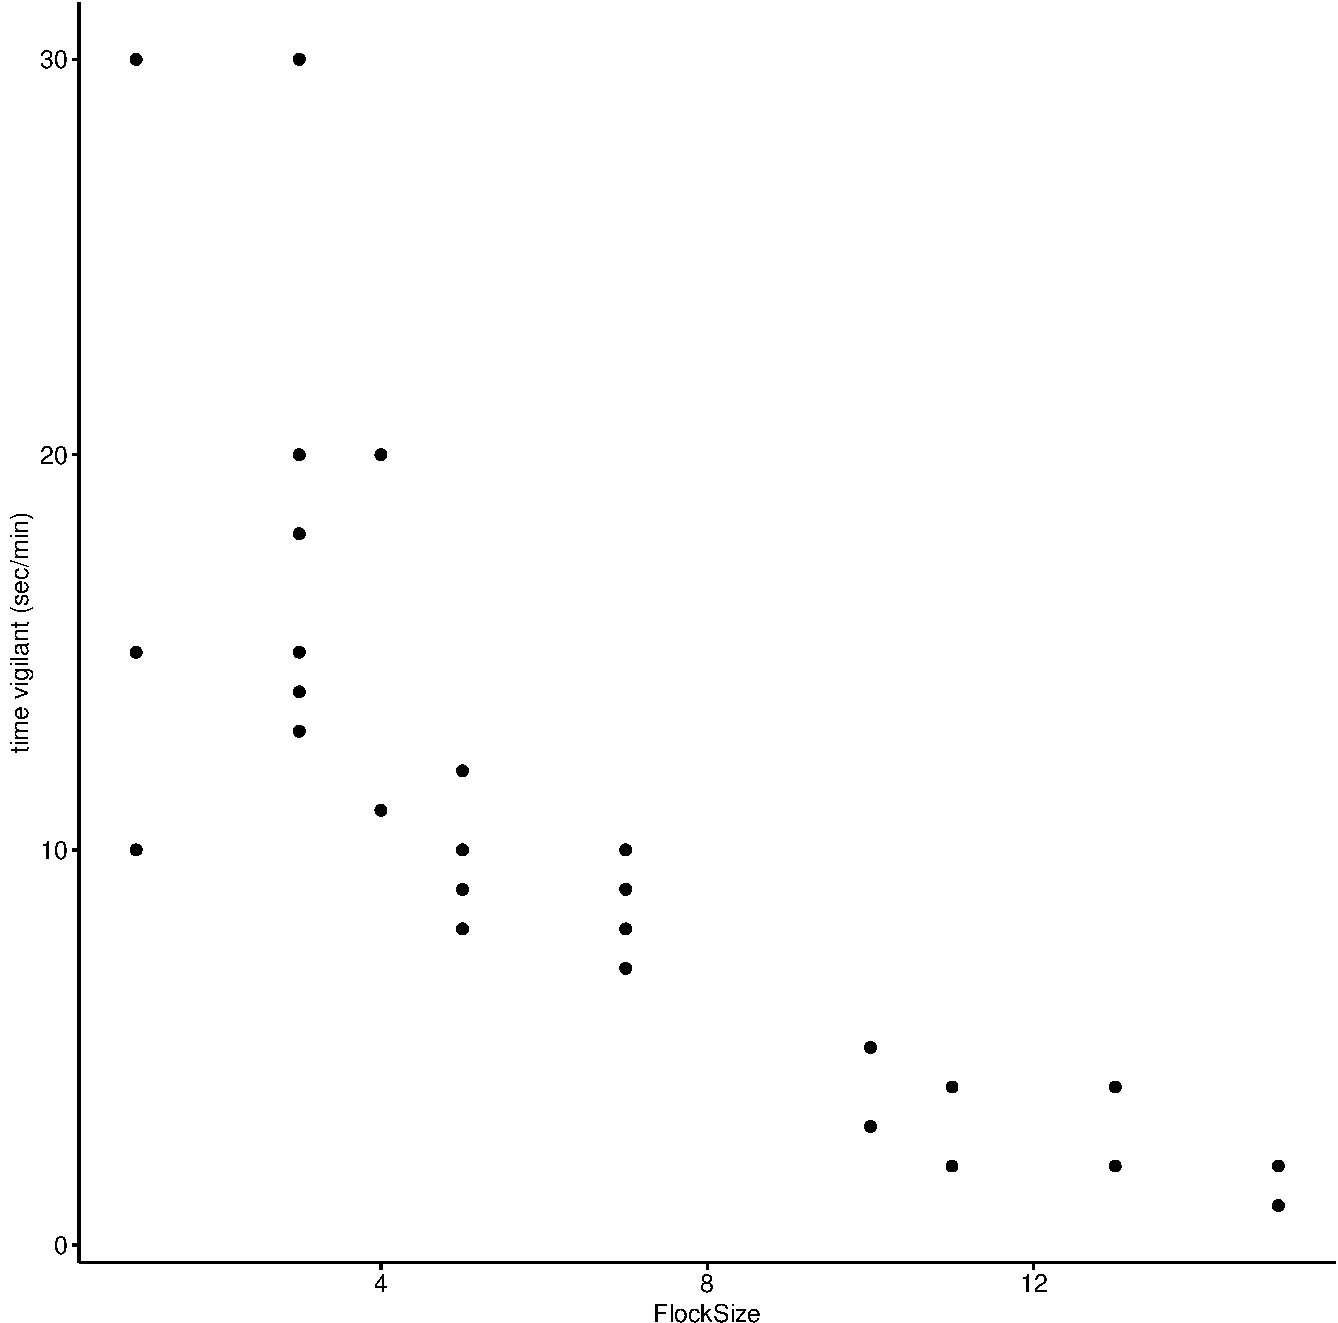
\includegraphics{behaviouR-R-package-tutorials_files/figure-latex/unnamed-chunk-96-1.pdf}

Now let's add a trend line to see if there is a relationship between flock size and the duration of vigilance.

\begin{Shaded}
\begin{Highlighting}[]
\CommentTok{# Scatterplot of duration of vigilance behavior in our data with a trend line.}

\KeywordTok{ggscatter}\NormalTok{(}\DataTypeTok{data=}\NormalTok{BarnacleGooseData,}\DataTypeTok{x=}\StringTok{'FlockSize'}\NormalTok{,}\DataTypeTok{y=}\StringTok{'TimeSecHeadUp'}\NormalTok{,}\DataTypeTok{add=}\StringTok{'reg.line'}\NormalTok{)}\OperatorTok{+}
\StringTok{  }\KeywordTok{ylab}\NormalTok{(}\StringTok{'time vigilant (sec/min)'}\NormalTok{)}
\end{Highlighting}
\end{Shaded}

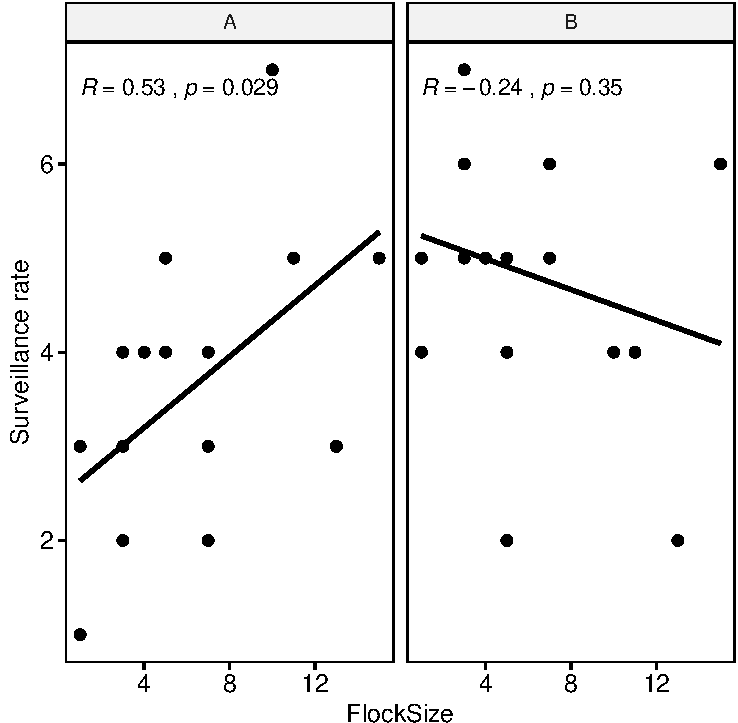
\includegraphics{behaviouR-R-package-tutorials_files/figure-latex/unnamed-chunk-97-1.pdf}

Let's see if there were any differences between you and your partner. We will also add the command `cor.coef = T' which will give us the correlation coefficient (R) along with an associated p-value.

\begin{Shaded}
\begin{Highlighting}[]
\CommentTok{# }\AlertTok{NOTE}\CommentTok{: The data here are simulated so your plots should look different}
\KeywordTok{ggscatter}\NormalTok{(}\DataTypeTok{data=}\NormalTok{BarnacleGooseData,}\DataTypeTok{x=}\StringTok{'FlockSize'}\NormalTok{,}\DataTypeTok{y=}\StringTok{'TimeSecHeadUp'}\NormalTok{,}\DataTypeTok{add=}\StringTok{'reg.line'}\NormalTok{,}
          \DataTypeTok{facet.by =} \StringTok{'Partner'}\NormalTok{,}\DataTypeTok{cor.coef =}\NormalTok{ T)}\OperatorTok{+}
\StringTok{  }\KeywordTok{ylab}\NormalTok{(}\StringTok{'time vigilant (sec/min)'}\NormalTok{)}
\end{Highlighting}
\end{Shaded}

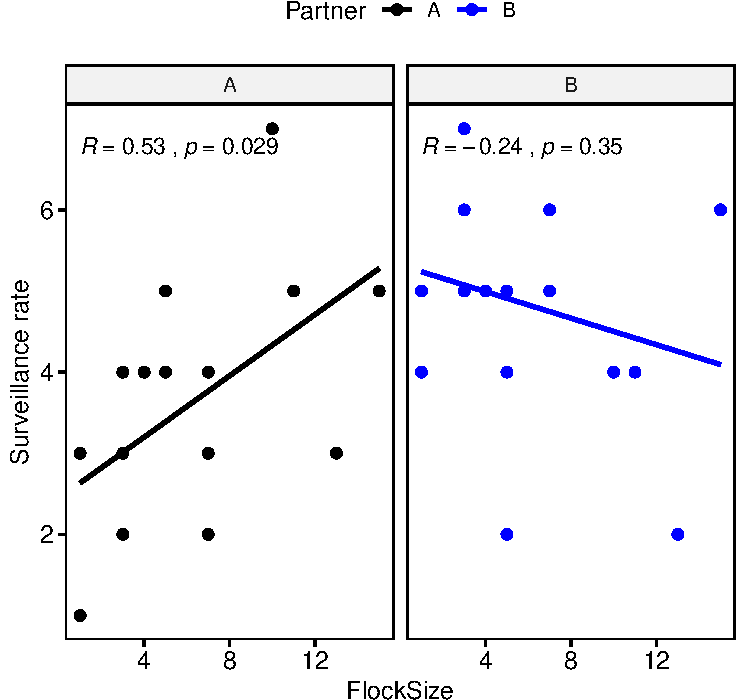
\includegraphics{behaviouR-R-package-tutorials_files/figure-latex/unnamed-chunk-98-1.pdf}

Let's plot you and your partner's data in different colors.

\begin{Shaded}
\begin{Highlighting}[]
\KeywordTok{ggscatter}\NormalTok{(}\DataTypeTok{data=}\NormalTok{BarnacleGooseData,}\DataTypeTok{x=}\StringTok{'FlockSize'}\NormalTok{,}\DataTypeTok{y=}\StringTok{'TimeSecHeadUp'}\NormalTok{,}\DataTypeTok{add=}\StringTok{'reg.line'}\NormalTok{,}
          \DataTypeTok{facet.by =} \StringTok{'Partner'}\NormalTok{, }\DataTypeTok{color=}\StringTok{'Partner'}\NormalTok{, }\DataTypeTok{cor.coef =}\NormalTok{ T,}
          \DataTypeTok{palette =}\KeywordTok{c}\NormalTok{(}\StringTok{'black'}\NormalTok{,}\StringTok{'blue'}\NormalTok{))}\OperatorTok{+}
\StringTok{            }\KeywordTok{ylab}\NormalTok{(}\StringTok{'time vigilant (sec/min)'}\NormalTok{)}
\end{Highlighting}
\end{Shaded}

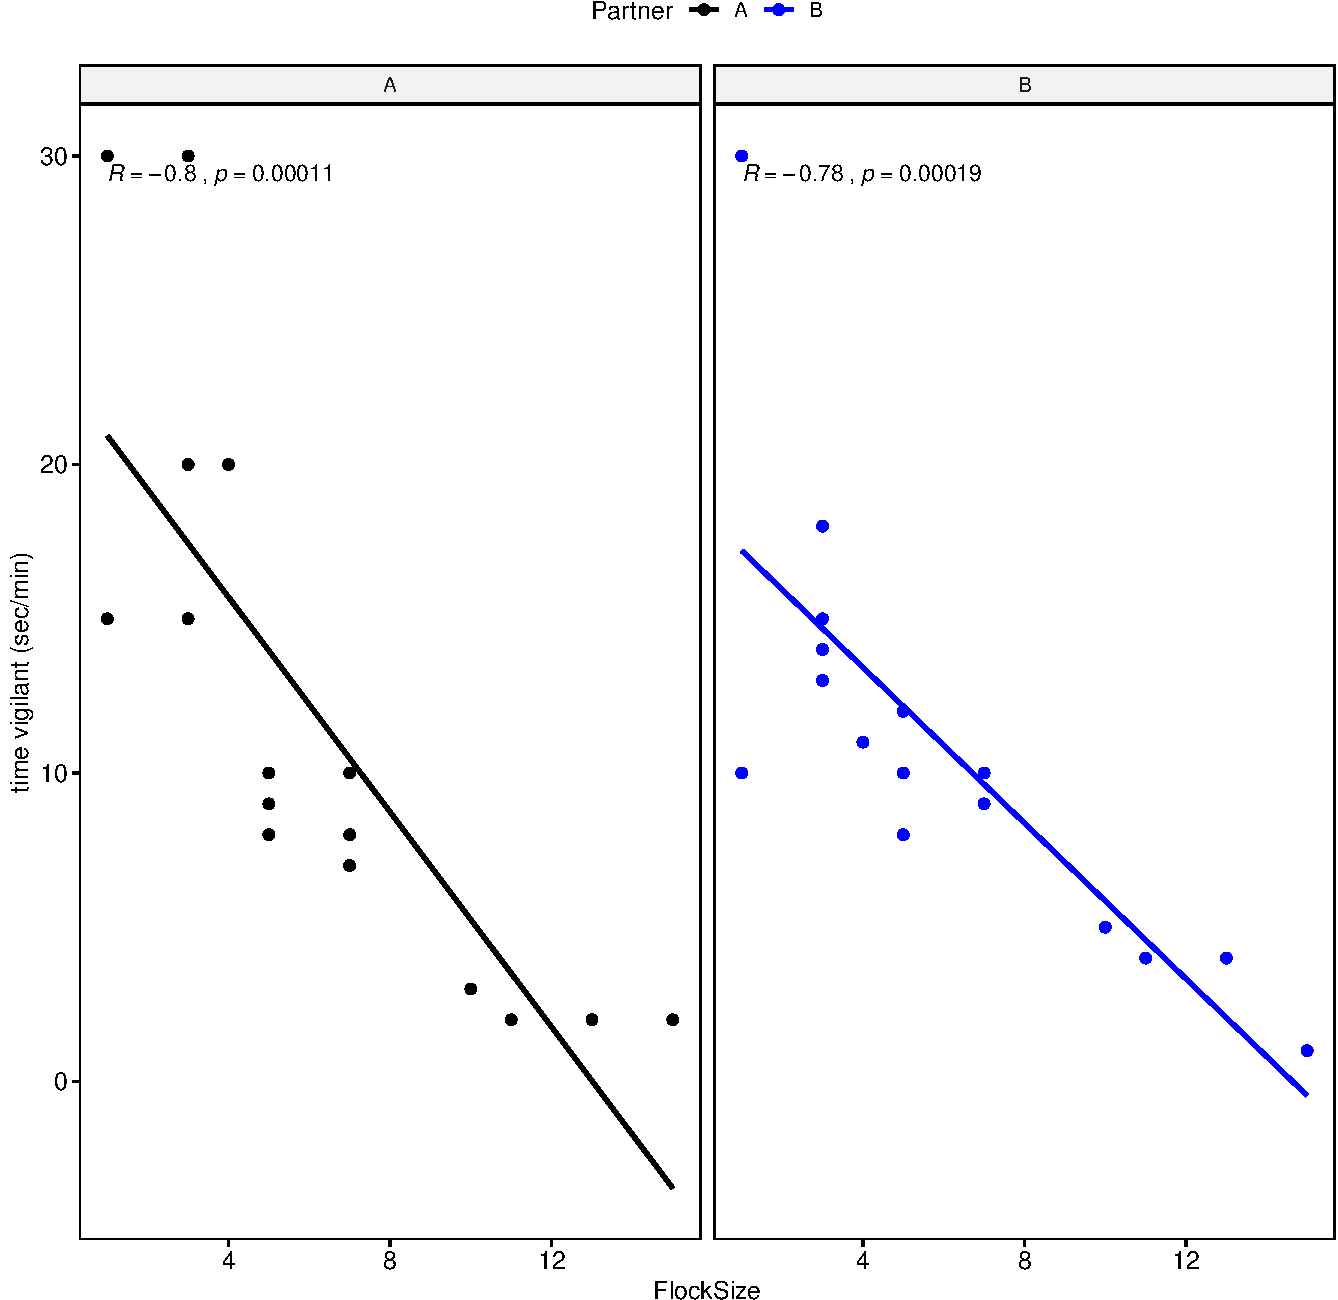
\includegraphics{behaviouR-R-package-tutorials_files/figure-latex/unnamed-chunk-99-1.pdf}

As before we will create a null model and then a model with flock size as a predictor and compare them using AIC. We will not use a Poisson distribution here because our outcome variable is continuous.

\begin{Shaded}
\begin{Highlighting}[]
\CommentTok{# This is our null model}
\NormalTok{VigilanceNullModel <-}\StringTok{ }\NormalTok{lme4}\OperatorTok{::}\KeywordTok{lmer}\NormalTok{(TimeSecHeadUp }\OperatorTok{~}\StringTok{ }\NormalTok{(}\DecValTok{1}\OperatorTok{|}\NormalTok{Partner), }\DataTypeTok{data=}\NormalTok{BarnacleGooseData)}

\CommentTok{# This is our model with flock size as a predictor duration of vigilance}
\NormalTok{VigilanceModel <-}\StringTok{ }\NormalTok{lme4}\OperatorTok{::}\KeywordTok{lmer}\NormalTok{(TimeSecHeadUp }\OperatorTok{~}\StringTok{ }\NormalTok{FlockSize }\OperatorTok{+}\StringTok{ }\NormalTok{(}\DecValTok{1}\OperatorTok{|}\NormalTok{Partner) ,}\DataTypeTok{data=}\NormalTok{BarnacleGooseData)}

\CommentTok{# Now we compare the models using AIC}
\NormalTok{bbmle}\OperatorTok{::}\KeywordTok{AICtab}\NormalTok{(VigilanceNullModel,VigilanceModel)}
\end{Highlighting}
\end{Shaded}

\begin{verbatim}
##                    dAIC df
## VigilanceModel      0.0 4 
## VigilanceNullModel 28.1 3
\end{verbatim}

\#\textbf{Question 3.} How do you interpret the results of your model selection? Was there a relationship between flock size and duration of vigilance behavior?

\hypertarget{part-2-meerkat-data-revisted}{%
\section*{Part 2: Meerkat data revisted}\label{part-2-meerkat-data-revisted}}
\addcontentsline{toc}{section}{Part 2: Meerkat data revisted}

Please upload your meerkat scan data to this project and delete the existing datasheet.

\begin{Shaded}
\begin{Highlighting}[]
\NormalTok{MeerkatScanData <-}\StringTok{ }\KeywordTok{read.csv}\NormalTok{(}\StringTok{'MeerkatScanData.csv'}\NormalTok{)}
\end{Highlighting}
\end{Shaded}

As before we will turn our NA values to zero

\begin{Shaded}
\begin{Highlighting}[]
\NormalTok{MeerkatScanData[}\KeywordTok{is.na}\NormalTok{(MeerkatScanData)] <-}\StringTok{ '0'}
\end{Highlighting}
\end{Shaded}

We will remove the time and out of sight columns as we do not need them

\begin{Shaded}
\begin{Highlighting}[]
\NormalTok{MeerkatScanData <-}\StringTok{ }\NormalTok{dplyr}\OperatorTok{::}\KeywordTok{select}\NormalTok{(MeerkatScanData,}\OperatorTok{-}\KeywordTok{c}\NormalTok{(Time,OutOfSight))}
\end{Highlighting}
\end{Shaded}

We need to reformat our data so that we can plot it

\begin{Shaded}
\begin{Highlighting}[]
\NormalTok{MeerkatScanDataSummaryLong <-}\StringTok{ }\NormalTok{reshape2}\OperatorTok{::}\KeywordTok{melt}\NormalTok{(MeerkatScanData, }\DataTypeTok{id.vars=}\KeywordTok{c}\NormalTok{(}\StringTok{"Treatment"}\NormalTok{, }\StringTok{"Partner"}\NormalTok{))}
\end{Highlighting}
\end{Shaded}

Here we add more informative column names

\begin{Shaded}
\begin{Highlighting}[]
\KeywordTok{colnames}\NormalTok{(MeerkatScanDataSummaryLong) <-}\StringTok{ }\KeywordTok{c}\NormalTok{(}\StringTok{'Treatment'}\NormalTok{,}\StringTok{'Partner'}\NormalTok{,}
                                          \StringTok{'BehavioralState'}\NormalTok{,}\StringTok{'InstancesOfBehavior'}\NormalTok{)}
\end{Highlighting}
\end{Shaded}

We need to tell R that our outcome variable is not categorical but numeric

\begin{Shaded}
\begin{Highlighting}[]
\NormalTok{MeerkatScanDataSummaryLong}\OperatorTok{$}\NormalTok{InstancesOfBehavior <-}\StringTok{ }
\StringTok{  }\KeywordTok{as.numeric}\NormalTok{(MeerkatScanDataSummaryLong}\OperatorTok{$}\NormalTok{InstancesOfBehavior)}
\end{Highlighting}
\end{Shaded}

Now we plot our data.

\begin{Shaded}
\begin{Highlighting}[]
\KeywordTok{ggboxplot}\NormalTok{(MeerkatScanDataSummaryLong,}\DataTypeTok{x=}\StringTok{'Treatment'}\NormalTok{,}
          \DataTypeTok{y=}\StringTok{'InstancesOfBehavior'}\NormalTok{, }\DataTypeTok{fill =} \StringTok{'BehavioralState'}\NormalTok{)}\OperatorTok{+}\KeywordTok{scale_fill_manual}\NormalTok{(}\DataTypeTok{values =} \KeywordTok{c}\NormalTok{(}\StringTok{'red'}\NormalTok{,}\StringTok{'white'}\NormalTok{,}\StringTok{'black'}\NormalTok{))}
\end{Highlighting}
\end{Shaded}

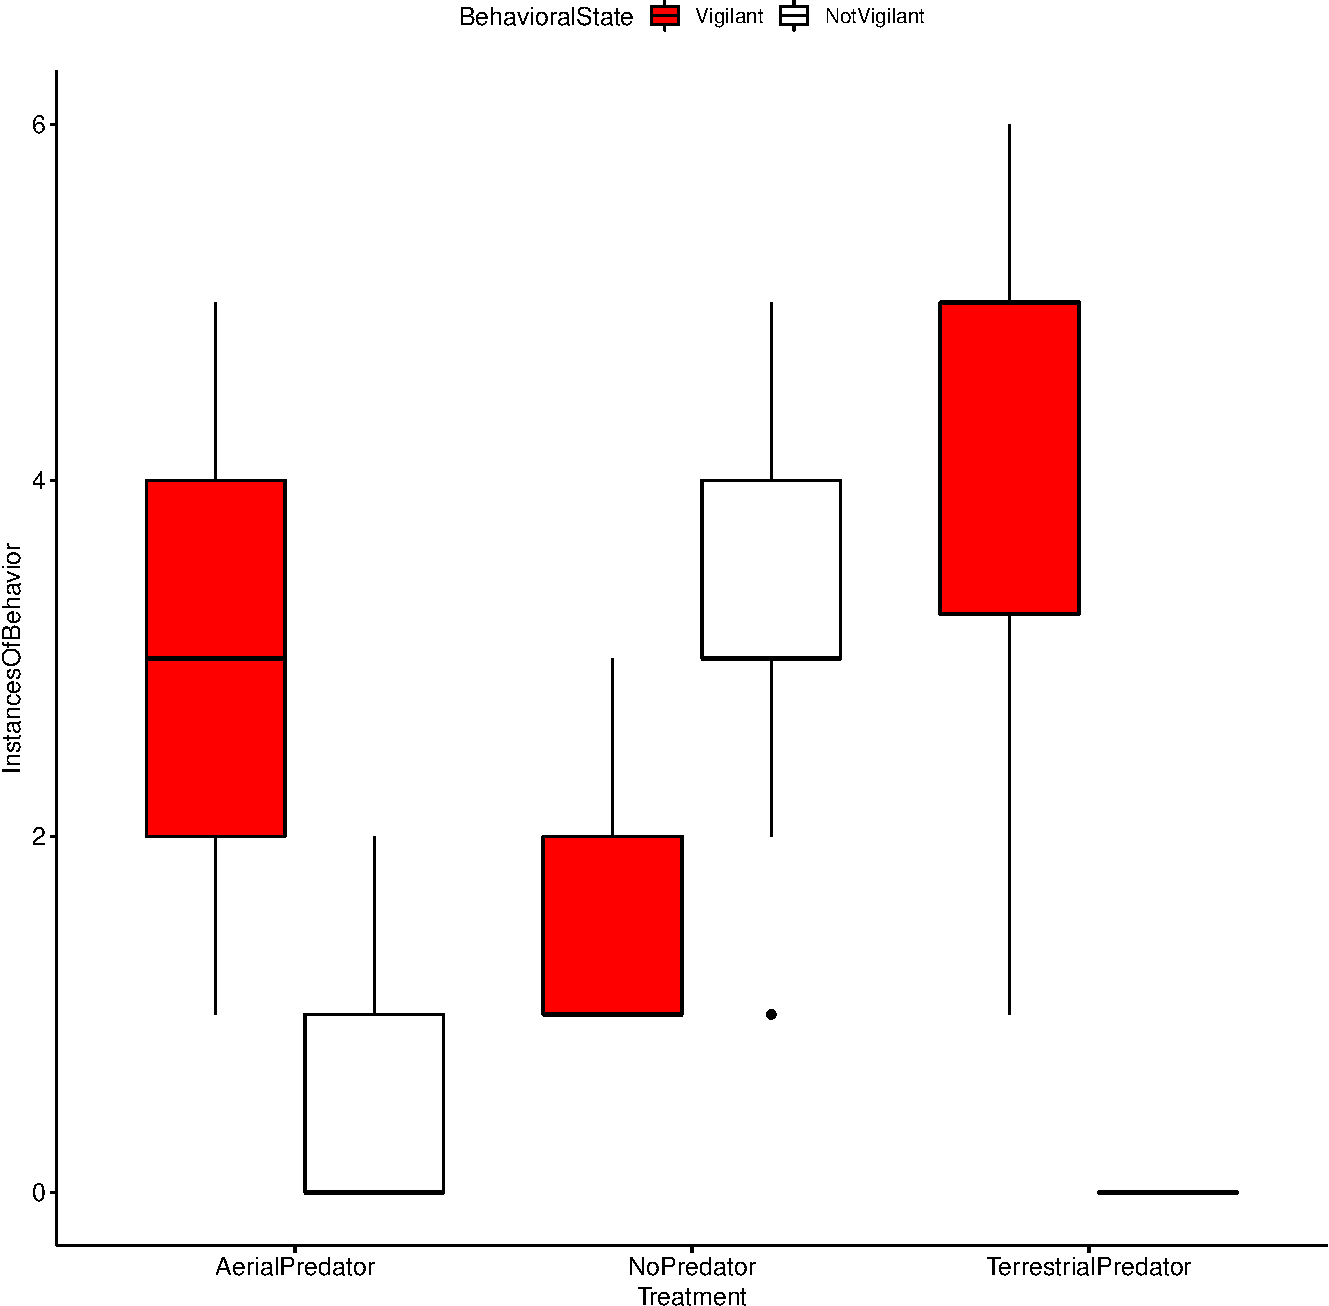
\includegraphics{behaviouR-R-package-tutorials_files/figure-latex/unnamed-chunk-108-1.pdf}

\textbf{Question 4.} Based on your inspection of the boxplots, are there any major differences between treatment groups?

Now we will test to see if there were differences in vigilance behaviors across treatments.

\begin{Shaded}
\begin{Highlighting}[]
\CommentTok{# First we subset our data so that it only includes the vigilant category}
\NormalTok{MeerkatScanDataVigilantOnly <-}\StringTok{ }\KeywordTok{subset}\NormalTok{(MeerkatScanDataSummaryLong,}
\NormalTok{                                      BehavioralState}\OperatorTok{==}\StringTok{'Vigilant'}\NormalTok{ )}

\CommentTok{# R can be picky about the format of data, so we use this command to tell R that treatment group is a factor}
\NormalTok{MeerkatScanDataVigilantOnly}\OperatorTok{$}\NormalTok{Treatment <-}\StringTok{ }
\StringTok{  }\KeywordTok{as.factor}\NormalTok{(MeerkatScanDataVigilantOnly}\OperatorTok{$}\NormalTok{Treatment)}

\CommentTok{# Here we are reordering the levels of the factors. For our model selection we are interested in whether we see differences from the control (no predator) and the predator treatments, so here we are setting the no predator group as our reference group.}

\NormalTok{MeerkatScanDataVigilantOnly}\OperatorTok{$}\NormalTok{Treatment <-}\StringTok{ }
\StringTok{  }\KeywordTok{factor}\NormalTok{(MeerkatScanDataVigilantOnly}\OperatorTok{$}\NormalTok{Treatment, }\DataTypeTok{levels =} \KeywordTok{c}\NormalTok{(}\StringTok{"NoPredator"}\NormalTok{, }\StringTok{"AerialPredator"}\NormalTok{, }
                                                           \StringTok{"TerrestrialPredator"}\NormalTok{))}
\end{Highlighting}
\end{Shaded}

Now as before we will do model selection. Note that because our outcome variable (instances of behavior) is in the form of count data we use a poisson distribution.

\begin{Shaded}
\begin{Highlighting}[]
\CommentTok{# This is the null model.}
\NormalTok{MeerkatVigilanceNullModel <-}\StringTok{ }\KeywordTok{glm}\NormalTok{(InstancesOfBehavior }\OperatorTok{~}\StringTok{ }\DecValTok{1}\NormalTok{, }\DataTypeTok{family=}\NormalTok{poisson, }\DataTypeTok{data=}\NormalTok{MeerkatScanDataVigilantOnly)}

\CommentTok{# This is the model with treatment as a predictor of instances of vigilant behavior}
\NormalTok{MeerkatVigilanceModel <-}\StringTok{ }\KeywordTok{glm}\NormalTok{(InstancesOfBehavior }\OperatorTok{~}\StringTok{ }\NormalTok{Treatment, }\DataTypeTok{family=}\NormalTok{poisson,}\DataTypeTok{data=}\NormalTok{MeerkatScanDataVigilantOnly)}
\end{Highlighting}
\end{Shaded}

Now we compare the models using AIC

\begin{Shaded}
\begin{Highlighting}[]
\NormalTok{bbmle}\OperatorTok{::}\KeywordTok{AICtab}\NormalTok{(MeerkatVigilanceNullModel,MeerkatVigilanceModel)}
\end{Highlighting}
\end{Shaded}

\begin{verbatim}
##                           dAIC df
## MeerkatVigilanceModel      0.0 3 
## MeerkatVigilanceNullModel 59.2 1
\end{verbatim}

Here we will use the summary function to look at the estimates. There is a lot of information here but we want to focus on the `Estimate'. In particular we are interested in the estimates for `TreatmentAerialPredator' and `TreatmentTerrestrialPredator'. The estimate is showing the effect that these variables have on our outcome (instances of behavior), relative to our control (no predator).Therefore positive estimates indicate that there were more vigilance behaviors in aerial and terrestrial predator treatments.

\begin{Shaded}
\begin{Highlighting}[]
\KeywordTok{summary}\NormalTok{(MeerkatVigilanceModel)}
\end{Highlighting}
\end{Shaded}

\begin{verbatim}
## 
## Call:
## glm(formula = InstancesOfBehavior ~ Treatment, family = poisson, 
##     data = MeerkatScanDataVigilantOnly)
## 
## Deviance Residuals: 
##     Min       1Q   Median       3Q      Max  
## -1.9295  -0.3475  -0.1588   0.3696   1.1825  
## 
## Coefficients:
##                              Estimate Std. Error z value Pr(>|z|)    
## (Intercept)                    0.3285     0.1414   2.323   0.0202 *  
## TreatmentAerialPredator        0.8671     0.1685   5.145 2.68e-07 ***
## TreatmentTerrestrialPredator   1.1362     0.1582   7.182 6.86e-13 ***
## ---
## Signif. codes:  0 '***' 0.001 '**' 0.01 '*' 0.05 '.' 0.1 ' ' 1
## 
## (Dispersion parameter for poisson family taken to be 1)
## 
##     Null deviance: 100.802  on 117  degrees of freedom
## Residual deviance:  37.587  on 115  degrees of freedom
## AIC: 384.39
## 
## Number of Fisher Scoring iterations: 4
\end{verbatim}

A common way to visulize results such as these are coefficient plots. Here we are looking at the effect of `TreatmentAerialPredator' and `TreatmentTerrestrialPredator' relative to our control group. The reference or group is indicated by the vertical dashed line. So, we can interpret that because the coefficients are positive (and the confidence intervals don't overlap zero) that both terrestrial and aerial treatments lead to an increase in vigilant behaviors.

\begin{Shaded}
\begin{Highlighting}[]
\NormalTok{coefplot}\OperatorTok{::}\KeywordTok{coefplot}\NormalTok{(MeerkatVigilanceModel,}\DataTypeTok{intercept=}\NormalTok{F)}
\end{Highlighting}
\end{Shaded}

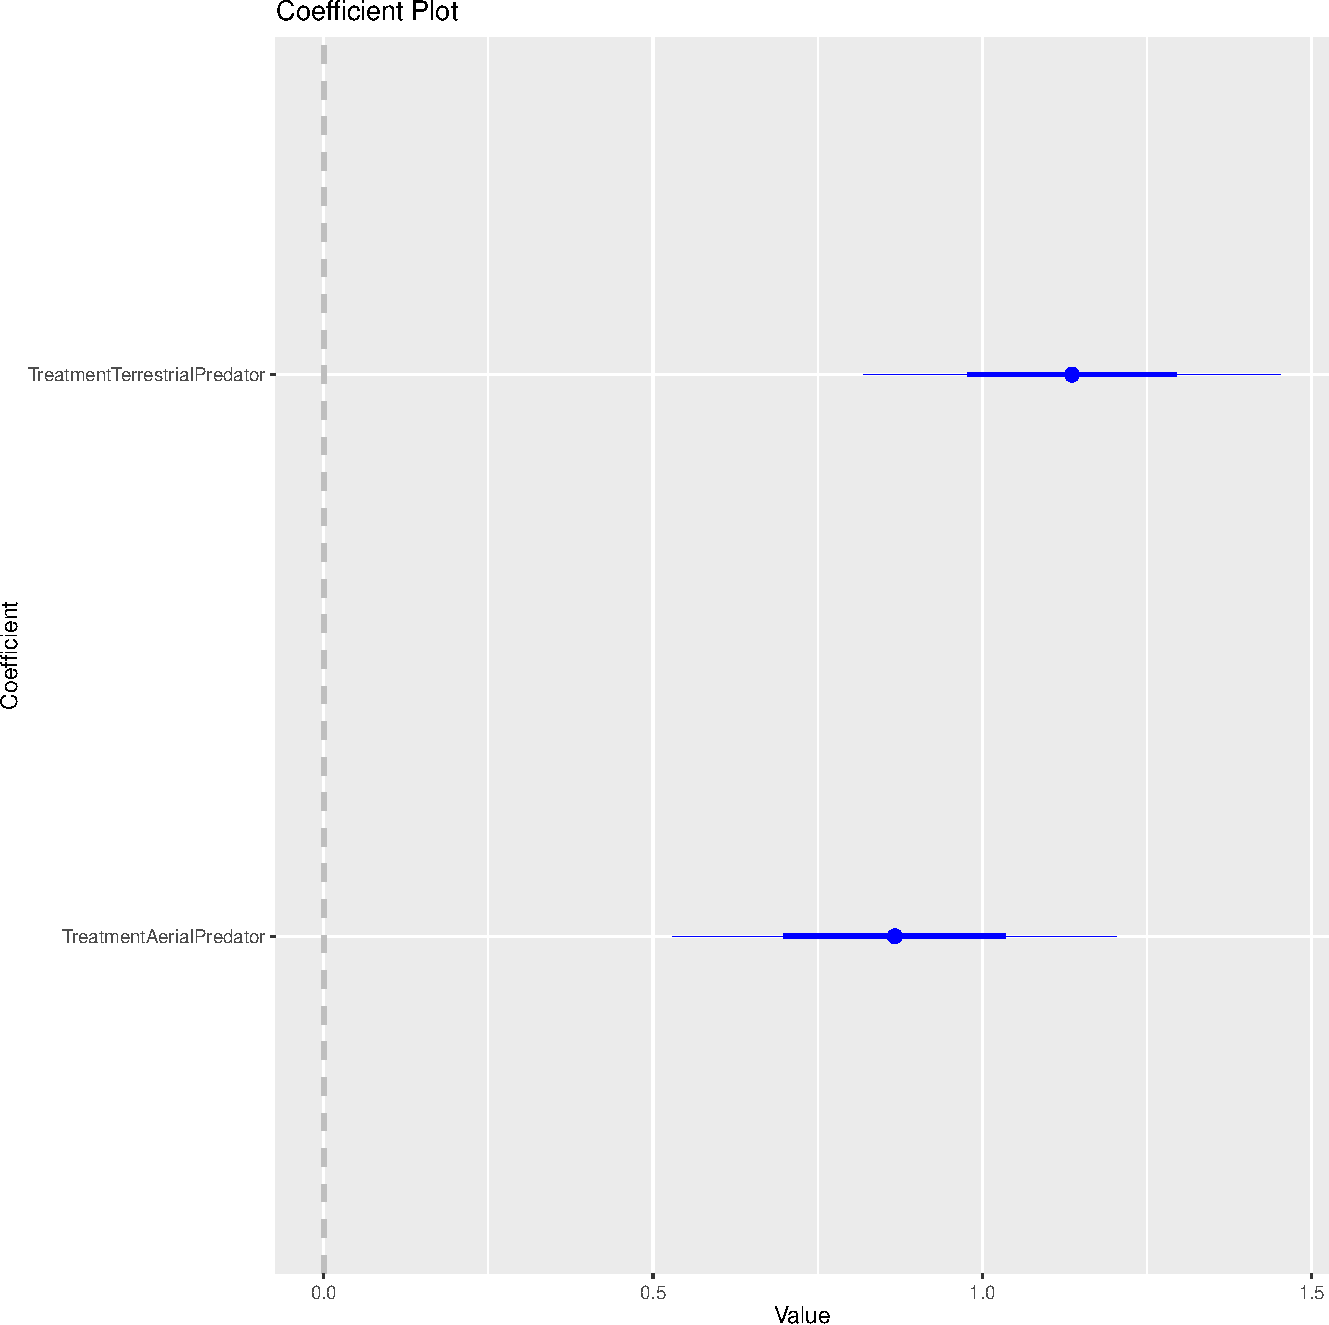
\includegraphics{behaviouR-R-package-tutorials_files/figure-latex/unnamed-chunk-113-1.pdf}

For reasons that will not go into here, I am not a fan of p-values or null hypothesis significance testing. There is a nice overview if you want to learn more here: \url{https://doi.org/10.1098/rsbl.2019.0174}. But,the model selection approach we used will lead to the same inference as the use of a one-way anova, an approach that you may be more familiar with.

Compute the analysis of variance

\begin{Shaded}
\begin{Highlighting}[]
\NormalTok{MeerkatAOV <-}\StringTok{ }\KeywordTok{aov}\NormalTok{(InstancesOfBehavior }\OperatorTok{~}\StringTok{ }\NormalTok{Treatment, }\DataTypeTok{data =}\NormalTok{ MeerkatScanDataVigilantOnly)}
\end{Highlighting}
\end{Shaded}

Here this will tell us if there are differences between groups. A significant p-value (\textless{} 0.05) indicates there are differences between treatment groups.

\begin{Shaded}
\begin{Highlighting}[]
\KeywordTok{summary}\NormalTok{(MeerkatAOV)}
\end{Highlighting}
\end{Shaded}

\begin{verbatim}
##              Df Sum Sq Mean Sq F value Pr(>F)    
## Treatment     2  176.0   88.02   87.03 <2e-16 ***
## Residuals   115  116.3    1.01                   
## ---
## Signif. codes:  0 '***' 0.001 '**' 0.01 '*' 0.05 '.' 0.1 ' ' 1
\end{verbatim}

Since the ANOVA test is significant, we can compute Tukey Honest Significant Differences test. Again, a significant p-value (\textless{} 0.05) indicates there are differences between treatments.

\begin{Shaded}
\begin{Highlighting}[]
\KeywordTok{TukeyHSD}\NormalTok{(MeerkatAOV)}
\end{Highlighting}
\end{Shaded}

\begin{verbatim}
##   Tukey multiple comparisons of means
##     95% family-wise confidence level
## 
## Fit: aov(formula = InstancesOfBehavior ~ Treatment, data = MeerkatScanDataVigilantOnly)
## 
## $Treatment
##                                        diff       lwr      upr   p adj
## AerialPredator-NoPredator          1.916667 1.3538432 2.479490 0.0e+00
## TerrestrialPredator-NoPredator     2.937198 2.4058425 3.468554 0.0e+00
## TerrestrialPredator-AerialPredator 1.020531 0.4891758 1.551887 3.8e-05
\end{verbatim}

\textbf{Question 5.} Based on your interpretation of the model selection and the coefficient plots were there differences between treatment groups (e.g.~control, terrestrial and aerial predators) in meerkat vigilance behavior?

\hypertarget{computer-lab-5.-estimating-population-density-and-biodiversity}{%
\chapter*{Computer Lab 5. Estimating Population Density and Biodiversity}\label{computer-lab-5.-estimating-population-density-and-biodiversity}}
\addcontentsline{toc}{chapter}{Computer Lab 5. Estimating Population Density and Biodiversity}

\begin{center}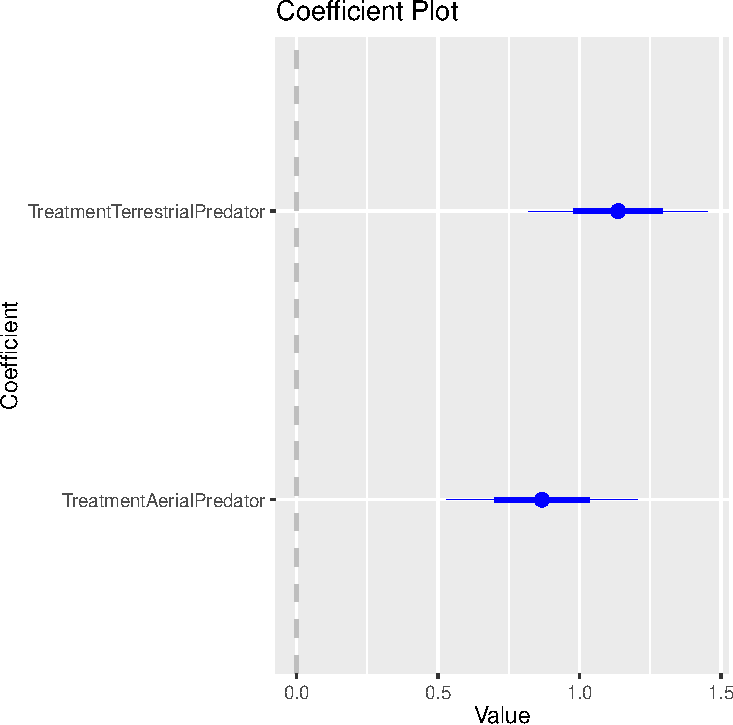
\includegraphics{behaviouR-R-package-tutorials_files/figure-latex/unnamed-chunk-117-1} \end{center}

\emph{Background}\\
In lecture this week we learned about population- and community- level interactions, and how they can influence individual and species-specific behavior. Differences in population density can lead to shifts in the proportion of different behavioral phenotypes in a population, and the presence of competitors of other species can shape the behavior of animals on shorter (ecological) and longer (evolutionary) time scales. In this lab you will become familiar with the ways that scientists estimate population density and biodiversity of terrestrial vertebrates.

\emph{Goals of the exercises}\\
The main goal(s) of today's lab are to:\\
1) Estimate population density of focal vertebrates from the field lab.\\
2) Learn the difference between alpha, beta and gamma diversity.\\
3) Compare population density and biodiversity across your sampling sites.

\emph{Getting started}\\
First we need to load the relevant packages for our data analysis. Packages contain all the functions that are needed for data analysis.

\begin{Shaded}
\begin{Highlighting}[]
\KeywordTok{library}\NormalTok{(behaviouR)}
\end{Highlighting}
\end{Shaded}

Then we read in our data

\begin{Shaded}
\begin{Highlighting}[]
\NormalTok{CensusData <-}\StringTok{ }\KeywordTok{read.csv}\NormalTok{(}\StringTok{'FieldLab5CensusData.csv'}\NormalTok{)}
\end{Highlighting}
\end{Shaded}

\hypertarget{part-1.-population-density-estimation.}{%
\section*{Part 1. Population density estimation.}\label{part-1.-population-density-estimation.}}
\addcontentsline{toc}{section}{Part 1. Population density estimation.}

First let's focus on your data.\\
NOTE: you need to change `A' to the name you used!

\begin{Shaded}
\begin{Highlighting}[]
\NormalTok{MyCensusData <-}\StringTok{ }\KeywordTok{subset}\NormalTok{(CensusData, Partner}\OperatorTok{==}\StringTok{'A'}\NormalTok{)}
\end{Highlighting}
\end{Shaded}

Now we will subset the data to focus on your focal species for density estimation. NOTE: in this example we are subsetting the data so that we only have the squirrels; you will need to change the code to subset based on your focal species!

\begin{Shaded}
\begin{Highlighting}[]
\NormalTok{MyCensusDataFocal <-}\StringTok{ }\KeywordTok{subset}\NormalTok{(MyCensusData, Species}\OperatorTok{==}\StringTok{'squirrel'}\NormalTok{)}
\end{Highlighting}
\end{Shaded}

Here we will determine the width of our sampling area by creating a histogram of perpendicular detection distances. We will identify the point where our detections start to dropoff. We will assume that after this point our ability to detect animals past that distance drops substantially, and including observations past this distance could potentially bias our results.

\begin{Shaded}
\begin{Highlighting}[]
\KeywordTok{hist}\NormalTok{(MyCensusDataFocal}\OperatorTok{$}\NormalTok{PerpendicularDistance,}\DataTypeTok{xlab=}\StringTok{'Perpendicular distance (D)'}\NormalTok{,}
  \DataTypeTok{ylab=}\StringTok{'Number of observations'}\NormalTok{,}\DataTypeTok{main=}\StringTok{''}\NormalTok{)}
\end{Highlighting}
\end{Shaded}

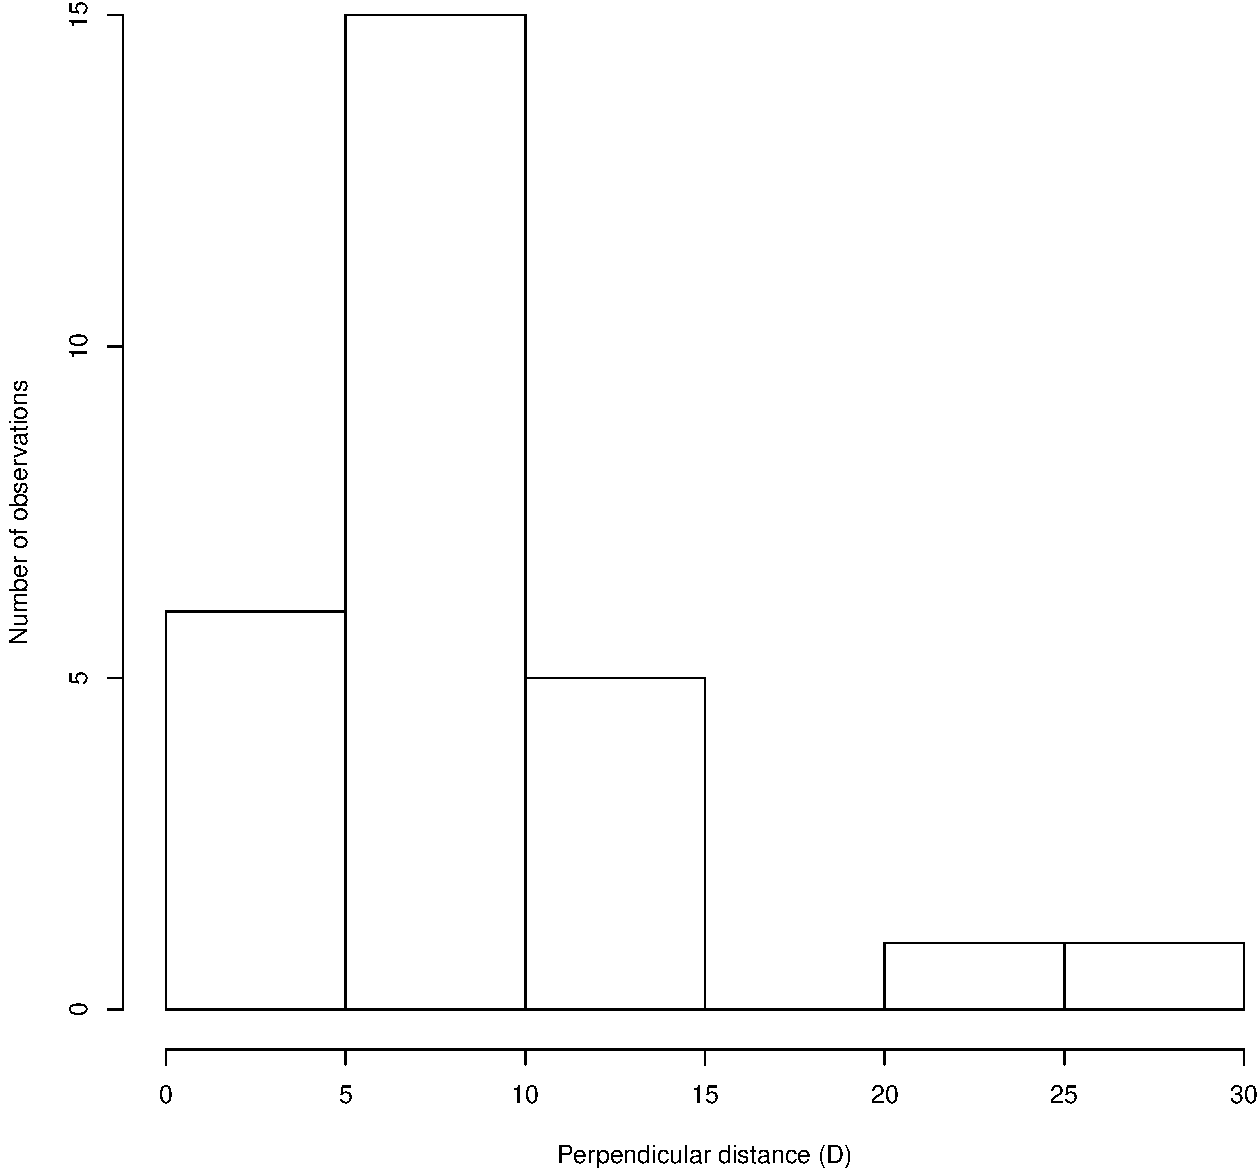
\includegraphics{behaviouR-R-package-tutorials_files/figure-latex/unnamed-chunk-123-1.pdf}

In this example there is a clear break between 15 and 20 meters, so we will only use observations that were within 15 meters.\\
NOTE: Your data will look different than this!

Change the value (in this example 15) to the cutoff point indicated in your data!

\begin{Shaded}
\begin{Highlighting}[]
\NormalTok{CutOffPoint <-}\StringTok{ }\DecValTok{15}
\end{Highlighting}
\end{Shaded}

\begin{Shaded}
\begin{Highlighting}[]
\CommentTok{# Here we subset our data so that it only includes detections that were within 15 meters of the census route}
\NormalTok{MyCensusDataFocalAdjusted <-}\StringTok{ }\KeywordTok{subset}\NormalTok{(MyCensusDataFocal,PerpendicularDistance }\OperatorTok{<}\NormalTok{CutOffPoint )}
\end{Highlighting}
\end{Shaded}

Now we need to subset by each site.\\
NOTE: You will need to change to the site names you used

\begin{Shaded}
\begin{Highlighting}[]
\NormalTok{MyCensusDataFocalSiteA <-}\StringTok{ }\KeywordTok{subset}\NormalTok{(MyCensusDataFocalAdjusted,Site}\OperatorTok{==}\StringTok{'SiteA'}\NormalTok{)}

\NormalTok{MyCensusDataFocalSiteB <-}\StringTok{ }\KeywordTok{subset}\NormalTok{(MyCensusDataFocalAdjusted,Site}\OperatorTok{==}\StringTok{'SiteB'}\NormalTok{)}
\end{Highlighting}
\end{Shaded}

Now we will calculate the population density based on our two surveys. Change the following to indicate the distance (in meters) of your survey for site A. This will be the actual straight-line distance you walked.

\begin{Shaded}
\begin{Highlighting}[]
\NormalTok{SiteACensusDistance <-}\StringTok{ }\DecValTok{500}
\end{Highlighting}
\end{Shaded}

Now we will calculate the area of our census. The sample area (a) is equal to the length of the transect multiplied by twice the width or a= 2wl. We divide by 1000 to convert our answer to square kilometers.

\begin{Shaded}
\begin{Highlighting}[]
\NormalTok{SiteACensusArea <-}\StringTok{ }\DecValTok{2}\OperatorTok{*}\NormalTok{SiteACensusDistance}\OperatorTok{*}\NormalTok{CutOffPoint}\OperatorTok{/}\DecValTok{1000}
\NormalTok{SiteACensusArea}
\end{Highlighting}
\end{Shaded}

\begin{verbatim}
## [1] 15
\end{verbatim}

Now we need to calculate the number of focal animals observed using the following code.

\begin{Shaded}
\begin{Highlighting}[]
\NormalTok{NumberFocalAnimalsSiteA <-}\StringTok{ }\KeywordTok{nrow}\NormalTok{(MyCensusDataFocalSiteA)}
\end{Highlighting}
\end{Shaded}

Then we can calculate the density by dividing the total number of animals we observed by the area we censused.

\begin{Shaded}
\begin{Highlighting}[]
\NormalTok{PopulationDensitySiteA <-NumberFocalAnimalsSiteA}\OperatorTok{/}\NormalTok{SiteACensusArea}
\NormalTok{PopulationDensitySiteA}
\end{Highlighting}
\end{Shaded}

\begin{verbatim}
## [1] 0.4666667
\end{verbatim}

Now we will calculate the population density based on our second survey. Change the following to indicate the distance (in meters) of your survey for site B.This will be the actual straight-line distance you walked.

\begin{Shaded}
\begin{Highlighting}[]
\NormalTok{SiteBCensusDistance <-}\StringTok{ }\DecValTok{500}
\end{Highlighting}
\end{Shaded}

Now we will calculate the area of our census. The sample area (a) is equal to the length of the transect multiplied by twice the width or a= 2wl.We divide by 1000 to convert our answer to square kilometers.

\begin{Shaded}
\begin{Highlighting}[]
\NormalTok{SiteBCensusArea <-}\StringTok{ }\DecValTok{2}\OperatorTok{*}\NormalTok{SiteBCensusDistance}\OperatorTok{*}\NormalTok{CutOffPoint}\OperatorTok{/}\DecValTok{1000}
\NormalTok{SiteBCensusArea}
\end{Highlighting}
\end{Shaded}

\begin{verbatim}
## [1] 15
\end{verbatim}

Now we need to calculate the number of animals using the following code.

\begin{Shaded}
\begin{Highlighting}[]
\NormalTok{NumberFocalAnimalsSiteB <-}\StringTok{ }\KeywordTok{nrow}\NormalTok{(MyCensusDataFocalSiteB)}
\end{Highlighting}
\end{Shaded}

Then we can calculate the density by dividing the total number of animals we observed by the area we censused.

\begin{Shaded}
\begin{Highlighting}[]
\NormalTok{PopulationDensitySiteB <-NumberFocalAnimalsSiteB}\OperatorTok{/}\NormalTok{SiteBCensusArea}
\NormalTok{PopulationDensitySiteB}
\end{Highlighting}
\end{Shaded}

\begin{verbatim}
## [1] 1.133333
\end{verbatim}

Now we can compare population density using the following code. The code below asks if the population density of site A was higher than site B?

\begin{Shaded}
\begin{Highlighting}[]
\NormalTok{PopulationDensitySiteA }\OperatorTok{>}\StringTok{ }\NormalTok{PopulationDensitySiteB}
\end{Highlighting}
\end{Shaded}

\begin{verbatim}
## [1] FALSE
\end{verbatim}

The code below asks if the population density of site B was higher than site A?

\begin{Shaded}
\begin{Highlighting}[]
\NormalTok{PopulationDensitySiteB }\OperatorTok{>}\StringTok{ }\NormalTok{PopulationDensitySiteA}
\end{Highlighting}
\end{Shaded}

\begin{verbatim}
## [1] TRUE
\end{verbatim}

\textbf{Question 1}. What were the population density estimates (reported as number of individuals per square kilometer) for your two sites? Do your results of the population density estimates match your predictions? Why or why not?

\hypertarget{part-2.-comparing-biodiversity.}{%
\section*{Part 2. Comparing biodiversity.}\label{part-2.-comparing-biodiversity.}}
\addcontentsline{toc}{section}{Part 2. Comparing biodiversity.}

\hypertarget{alpha-diversity.}{%
\subsection*{Alpha diversity.}\label{alpha-diversity.}}
\addcontentsline{toc}{subsection}{Alpha diversity.}

First, we will estimate the alpha diversity, or the diversity within a particular area or ecosystem. The alpha diversity is simply the number of different species present at each site.

Here we subset by partner and site A (you may need to change these!)

\begin{Shaded}
\begin{Highlighting}[]
\NormalTok{MyCensusDataSiteA <-}\StringTok{ }\KeywordTok{subset}\NormalTok{(MyCensusData,Partner}\OperatorTok{==}\StringTok{'A'} \OperatorTok{&}\StringTok{ }\NormalTok{Site}\OperatorTok{==}\StringTok{'SiteA'}\NormalTok{)}

\CommentTok{# What were the unique species present?}
\KeywordTok{unique}\NormalTok{(MyCensusDataSiteA}\OperatorTok{$}\NormalTok{Species)}
\end{Highlighting}
\end{Shaded}

\begin{verbatim}
## [1] cardinal  blackird1 rabbit    deer      squirrel  crow     
## Levels: blackird1 cardinal crow deer rabbit squirrel
\end{verbatim}

\begin{Shaded}
\begin{Highlighting}[]
\CommentTok{# How many unique species were there?}
\NormalTok{SiteANumberSpecies <-}\StringTok{ }\KeywordTok{length}\NormalTok{(}\KeywordTok{unique}\NormalTok{(MyCensusDataSiteA}\OperatorTok{$}\NormalTok{Species))}
\NormalTok{SiteANumberSpecies}
\end{Highlighting}
\end{Shaded}

\begin{verbatim}
## [1] 6
\end{verbatim}

Here we subset by partner and site B (you may need to change these!)

\begin{Shaded}
\begin{Highlighting}[]
\NormalTok{MyCensusDataSiteB <-}\StringTok{ }\KeywordTok{subset}\NormalTok{(MyCensusData,Partner}\OperatorTok{==}\StringTok{'A'} \OperatorTok{&}\StringTok{ }\NormalTok{Site}\OperatorTok{==}\StringTok{'SiteB'}\NormalTok{)}

\CommentTok{# What were the unique species present?}
\KeywordTok{unique}\NormalTok{(MyCensusDataSiteB}\OperatorTok{$}\NormalTok{Species)}
\end{Highlighting}
\end{Shaded}

\begin{verbatim}
## [1] squirrel  blackird1 rabbit    deer      crow     
## Levels: blackird1 cardinal crow deer rabbit squirrel
\end{verbatim}

\begin{Shaded}
\begin{Highlighting}[]
\CommentTok{# How many unique species were there?}
\NormalTok{SiteBNumberSpecies <-}\StringTok{ }\KeywordTok{length}\NormalTok{(}\KeywordTok{unique}\NormalTok{(MyCensusDataSiteB}\OperatorTok{$}\NormalTok{Species))}
\NormalTok{SiteBNumberSpecies}
\end{Highlighting}
\end{Shaded}

\begin{verbatim}
## [1] 5
\end{verbatim}

\textbf{Question 2}. Which of your sites had higher species richness (i.e.~number of species)?

\hypertarget{beta-diversity.}{%
\subsection*{Beta diversity.}\label{beta-diversity.}}
\addcontentsline{toc}{subsection}{Beta diversity.}

Now we will estimate beta diversity, which estimates changes in species diversity between ecosystems or along environmental gradients.

\begin{Shaded}
\begin{Highlighting}[]
\CommentTok{# This code tells us which species both sites have in common}
\KeywordTok{intersect}\NormalTok{(}\KeywordTok{unique}\NormalTok{(MyCensusDataSiteA}\OperatorTok{$}\NormalTok{Species),}\KeywordTok{unique}\NormalTok{(MyCensusDataSiteB}\OperatorTok{$}\NormalTok{Species))}
\end{Highlighting}
\end{Shaded}

\begin{verbatim}
## [1] "blackird1" "rabbit"    "deer"      "squirrel"  "crow"
\end{verbatim}

\begin{Shaded}
\begin{Highlighting}[]
\CommentTok{# Now we calculate the number of species in common}
\NormalTok{SpeciesInCommonBothSites <-}\StringTok{ }\KeywordTok{length}\NormalTok{(}\KeywordTok{intersect}\NormalTok{(}\KeywordTok{unique}\NormalTok{(MyCensusDataSiteA}\OperatorTok{$}\NormalTok{Species),}\KeywordTok{unique}\NormalTok{(MyCensusDataSiteB}\OperatorTok{$}\NormalTok{Species))}
\NormalTok{)}
\NormalTok{SpeciesInCommonBothSites}
\end{Highlighting}
\end{Shaded}

\begin{verbatim}
## [1] 5
\end{verbatim}

To investigate community similarity we will calculate Sørenson's index; a value of 1 means exactly the same number of species a value of 0 means no overlap.

Beta diversity = 2c / S1 + S2\\
Where c is the number of species the sites have in common, S1 is the number of species at the first site and S2 is the number of species at the second site

\begin{Shaded}
\begin{Highlighting}[]
\DecValTok{2}\OperatorTok{*}\NormalTok{SpeciesInCommonBothSites}\OperatorTok{/}\StringTok{ }\NormalTok{(SiteANumberSpecies}\OperatorTok{+}\NormalTok{SiteBNumberSpecies)}
\end{Highlighting}
\end{Shaded}

\begin{verbatim}
## [1] 0.9090909
\end{verbatim}

Now we will use your partner's data to estimate alpha diversity

\begin{Shaded}
\begin{Highlighting}[]
\NormalTok{MyPartnersCensusDataSiteA <-}\StringTok{ }\KeywordTok{subset}\NormalTok{(CensusData,Partner}\OperatorTok{==}\StringTok{'B'} \OperatorTok{&}\StringTok{ }\NormalTok{Site}\OperatorTok{==}\StringTok{'SiteC'}\NormalTok{)}
\KeywordTok{unique}\NormalTok{(MyPartnersCensusDataSiteA}\OperatorTok{$}\NormalTok{Species)}
\end{Highlighting}
\end{Shaded}

\begin{verbatim}
## [1] squirrel crow    
## Levels: blackird1 cardinal crow deer rabbit squirrel
\end{verbatim}

\begin{Shaded}
\begin{Highlighting}[]
\KeywordTok{length}\NormalTok{(}\KeywordTok{unique}\NormalTok{(MyPartnersCensusDataSiteA}\OperatorTok{$}\NormalTok{Species))}
\end{Highlighting}
\end{Shaded}

\begin{verbatim}
## [1] 2
\end{verbatim}

\begin{Shaded}
\begin{Highlighting}[]
\NormalTok{SiteANumberSpecies <-}\StringTok{ }\KeywordTok{length}\NormalTok{(}\KeywordTok{unique}\NormalTok{(MyPartnersCensusDataSiteA}\OperatorTok{$}\NormalTok{Species))}
\NormalTok{SiteANumberSpecies}
\end{Highlighting}
\end{Shaded}

\begin{verbatim}
## [1] 2
\end{verbatim}

\begin{Shaded}
\begin{Highlighting}[]
\NormalTok{MyPartnersCensusDataSiteB <-}\StringTok{ }\KeywordTok{subset}\NormalTok{(CensusData,Partner}\OperatorTok{==}\StringTok{'B'} \OperatorTok{&}\StringTok{ }\NormalTok{Site}\OperatorTok{==}\StringTok{'SiteD'}\NormalTok{)}
\KeywordTok{unique}\NormalTok{(MyPartnersCensusDataSiteB}\OperatorTok{$}\NormalTok{Species)}
\end{Highlighting}
\end{Shaded}

\begin{verbatim}
## [1] squirrel
## Levels: blackird1 cardinal crow deer rabbit squirrel
\end{verbatim}

\begin{Shaded}
\begin{Highlighting}[]
\KeywordTok{length}\NormalTok{(}\KeywordTok{unique}\NormalTok{(MyPartnersCensusDataSiteB}\OperatorTok{$}\NormalTok{Species))}
\end{Highlighting}
\end{Shaded}

\begin{verbatim}
## [1] 1
\end{verbatim}

\begin{Shaded}
\begin{Highlighting}[]
\NormalTok{SiteBNumberSpecies <-}\StringTok{ }\KeywordTok{length}\NormalTok{(}\KeywordTok{unique}\NormalTok{(MyPartnersCensusDataSiteB}\OperatorTok{$}\NormalTok{Species))}
\NormalTok{SiteBNumberSpecies}
\end{Highlighting}
\end{Shaded}

\begin{verbatim}
## [1] 1
\end{verbatim}

\textbf{Question 3}. How did the alpha diversity of each of your sites compare with that of your partner?

\hypertarget{gamma-diversity}{%
\subsection*{Gamma diversity}\label{gamma-diversity}}
\addcontentsline{toc}{subsection}{Gamma diversity}

Gamma diversity is the total number of species over a large area or region; there are many different ways that this can be measured. The way we will do it is a bit of an oversimplification by simply comparing the number of species seen during the census at both locations.

First we subset by the first partner

\begin{Shaded}
\begin{Highlighting}[]
\NormalTok{MyCensusData <-}\StringTok{ }\KeywordTok{subset}\NormalTok{(CensusData, Partner}\OperatorTok{==}\StringTok{'A'}\NormalTok{)}
\KeywordTok{unique}\NormalTok{(MyCensusData}\OperatorTok{$}\NormalTok{Species)}
\end{Highlighting}
\end{Shaded}

\begin{verbatim}
## [1] cardinal  blackird1 rabbit    deer      squirrel  crow     
## Levels: blackird1 cardinal crow deer rabbit squirrel
\end{verbatim}

Then we plot the results

\begin{Shaded}
\begin{Highlighting}[]
\KeywordTok{gghistogram}\NormalTok{(}\DataTypeTok{data=}\NormalTok{MyCensusData, }\DataTypeTok{x=}\StringTok{'Species'}\NormalTok{,}\DataTypeTok{stat=}\StringTok{"count"}\NormalTok{)}
\end{Highlighting}
\end{Shaded}

\includegraphics{behaviouR-R-package-tutorials_files/figure-latex/unnamed-chunk-143-1.pdf}

Now we subset by the second partner

\begin{Shaded}
\begin{Highlighting}[]
\NormalTok{MyPartnersCensusData <-}\StringTok{ }\KeywordTok{subset}\NormalTok{(CensusData, Partner}\OperatorTok{==}\StringTok{'B'}\NormalTok{)}
\KeywordTok{unique}\NormalTok{(MyPartnersCensusData}\OperatorTok{$}\NormalTok{Species)}
\end{Highlighting}
\end{Shaded}

\begin{verbatim}
## [1] squirrel crow    
## Levels: blackird1 cardinal crow deer rabbit squirrel
\end{verbatim}

Then we plot the results

\begin{Shaded}
\begin{Highlighting}[]
\KeywordTok{gghistogram}\NormalTok{(}\DataTypeTok{data=}\NormalTok{MyPartnersCensusData, }\DataTypeTok{x=}\StringTok{'Species'}\NormalTok{,}\DataTypeTok{stat=}\StringTok{"count"}\NormalTok{)}
\end{Highlighting}
\end{Shaded}

\includegraphics{behaviouR-R-package-tutorials_files/figure-latex/unnamed-chunk-145-1.pdf}

Now we can plot all the data together, separated by partner

\begin{Shaded}
\begin{Highlighting}[]
\KeywordTok{gghistogram}\NormalTok{(}\DataTypeTok{data=}\NormalTok{CensusData, }\DataTypeTok{x=}\StringTok{'Species'}\NormalTok{,}\DataTypeTok{stat=}\StringTok{"count"}\NormalTok{,}
            \DataTypeTok{facet.by =} \StringTok{'Partner'}\NormalTok{,}\DataTypeTok{x.text.angle =}\DecValTok{90}\NormalTok{,}
            \DataTypeTok{fill=}\StringTok{'Partner'}\NormalTok{)}\OperatorTok{+}\KeywordTok{xlab}\NormalTok{(}\StringTok{'Species'}\NormalTok{)}\OperatorTok{+}\KeywordTok{ylab}\NormalTok{(}\StringTok{'Number of individuals'}\NormalTok{)}
\end{Highlighting}
\end{Shaded}

\includegraphics{behaviouR-R-package-tutorials_files/figure-latex/unnamed-chunk-146-1.pdf}

\textbf{Question 4}. How did the gamma diversity of your site compare with that of your partners?

\hypertarget{part-3.-biodiversity-indices-in-the-real-world.}{%
\section*{Part 3. Biodiversity indices in the real world.}\label{part-3.-biodiversity-indices-in-the-real-world.}}
\addcontentsline{toc}{section}{Part 3. Biodiversity indices in the real world.}

There are special packages in R that can measure different diversity indices, as biodiversity indices are tools many ecologists use. The package we will use is called `vegan'.

\begin{Shaded}
\begin{Highlighting}[]
\KeywordTok{library}\NormalTok{(vegan)}
\end{Highlighting}
\end{Shaded}

First we need to convert our data into a table that can be used to calculate the indices.

\begin{Shaded}
\begin{Highlighting}[]
\NormalTok{BiodiversityTable <-}\StringTok{ }\KeywordTok{table}\NormalTok{(CensusData}\OperatorTok{$}\NormalTok{Site,CensusData}\OperatorTok{$}\NormalTok{Species)}
\end{Highlighting}
\end{Shaded}

Simpson's Index (D) measures the probability that two individuals randomly selected from a sample will belong to the same species (or some category other than species). With this index, 1 represents infinite diversity and 0 means no diversity.

\begin{Shaded}
\begin{Highlighting}[]
\NormalTok{H <-}\StringTok{ }\KeywordTok{diversity}\NormalTok{(BiodiversityTable,}\DataTypeTok{index=}\StringTok{"simpson"}\NormalTok{)}
\NormalTok{H}
\end{Highlighting}
\end{Shaded}

\begin{verbatim}
##     SiteA     SiteB     SiteC     SiteD 
## 0.7962963 0.6728395 0.4444444 0.0000000
\end{verbatim}

Species evenness refers to how close in numbers each species is in an environment. We can calculate evenness using the following code. The value is constrained between 0 and 1, with communities that have a more even representation of species having values closer to 1.

\begin{Shaded}
\begin{Highlighting}[]
\NormalTok{J <-}\StringTok{ }\NormalTok{H}\OperatorTok{/}\KeywordTok{log}\NormalTok{(}\KeywordTok{specnumber}\NormalTok{(BiodiversityTable))}
\NormalTok{J}
\end{Highlighting}
\end{Shaded}

\begin{verbatim}
##     SiteA     SiteB     SiteC     SiteD 
## 0.4444214 0.4180587 0.6411978       NaN
\end{verbatim}

\textbf{Question 5}. Which of the four sites you analyzed was most diverse? Which was the most even? Why is it important to consider diversity and evenness when studying biodiversity?

\hypertarget{computer-lab-6.-analyzing-camera-trap-data.}{%
\chapter*{Computer Lab 6. Analyzing camera trap data.}\label{computer-lab-6.-analyzing-camera-trap-data.}}
\addcontentsline{toc}{chapter}{Computer Lab 6. Analyzing camera trap data.}

\begin{center}\includegraphics[width=0.8\linewidth]{behaviouR-R-package-tutorials_files/figure-latex/unnamed-chunk-151-1} \end{center}

\emph{Background}\\
In this lab we will use actual camera trap data collected in Serengeti National Park to investigate temporal niche partitioning. The camera trap data that we will use for this field lab comes from the `Snapshot Serengeti' project (\url{http://lila.science/datasets/snapshot-serengeti}). The scientists set out out 225 cameras within a 1,125 km2 area. The cameras have been deployed continuously since 2010, and the researchers recruited citizen scientists to help with classifying images (\url{https://www.zooniverse.org/projects/zooniverse/snapshot-serengeti}).

\emph{Goals of the exercises}\\
The main goal(s) of today's lab are to:\\
1) Understand the types of behavioral data that scientists can collect from camera trap photos.\\
2) Become familiar with one of the ways scientists can compare differences in activity patterns.\\
3) Think about interspecific interactions of predator-prey and potential competitors in the Serengeti.

\emph{Getting started}\\
First we need to load the relevant packages for our data analysis. Packages contain all the functions that are needed for data analysis.

\begin{Shaded}
\begin{Highlighting}[]
\KeywordTok{library}\NormalTok{(behaviouR)}
\KeywordTok{library}\NormalTok{(ggpubr)}
\end{Highlighting}
\end{Shaded}

\hypertarget{part-1-collect-serengeti-camera-trap-data}{%
\section*{Part 1: Collect Serengeti camera trap data}\label{part-1-collect-serengeti-camera-trap-data}}
\addcontentsline{toc}{section}{Part 1: Collect Serengeti camera trap data}

The original dataset includes over 2.65M sequences of camera trap images (totaling 7.1M images) from ten field seasons. As you can imagine that is a lot of data! For this lab we will focus on a subset of the data collected over the course of a few seasons.

We will be taking random subsets of the camera trap photos (the current default is 5 per season which you should change for your actual study), and we use `set.seed' to make sure that our results are reproducible.

\begin{Shaded}
\begin{Highlighting}[]
\KeywordTok{set.seed}\NormalTok{(}\DecValTok{2210}\NormalTok{)}
\end{Highlighting}
\end{Shaded}

We can use the following code to query the database by season to see which photos are available. The available seasons are 1-4, 6-8,10,11. This function will return a table with all of the available camera trap photos for a particular season. With camera trap data often times photos will be taken in a sequence (e.g.~if the animal is moving in front of the camera for a long time). The values in the table below include all photos in a sequence, but the code we use to download the photos only takes the first photo in a sequence. Therefore the sample sizes indicated in this table and the actual sample size may be different.

\begin{Shaded}
\begin{Highlighting}[]
\KeywordTok{CameraTrapAnnotations}\NormalTok{(}\DataTypeTok{season =} \DecValTok{1}\NormalTok{)}
\end{Highlighting}
\end{Shaded}

\begin{verbatim}
## 
##        aardvark        aardwolf          baboon     batearedfox         buffalo 
##             143              88             348             315            1455 
##        bushbuck         caracal         cheetah           civet          dikdik 
##              36              57             575              27             728 
##           eland        elephant   gazellegrants gazellethomsons           genet 
##             113            1687            4967           29705              28 
##         giraffe      guineafowl            hare      hartebeest    hippopotamus 
##            1923            3217             327            2139             340 
##     honeybadger    hyenaspotted    hyenastriped          impala          jackal 
##              42            2752             112             691             304 
##     koribustard         leopard      lionfemale        lionmale        mongoose 
##             591              38            1519             665             290 
##    monkeyvervet         ostrich       otherbird       porcupine        reedbuck 
##              64             211            2322             114             946 
##        reptiles      rhinoceros         rodents   secretarybird          serval 
##             357               6             129             198             174 
##            topi         warthog       waterbuck         wildcat      wildebeest 
##             428            2685              25              48             689 
##           zebra         zorilla 
##            5592               9
\end{verbatim}

For this lab you are going to choose two animals from the camera trap dataset. It could be a pair of animals that are predator and prey or two potential competitors. Once you decide on the two animals you want to compare you will make some predictions about how you think they will differ in their activity patterns.

Now we will use another function to download the camera trap photos and save them locally to our computer. You can change the season by changing the values for season (remember the available seasons are 1-4, 6-8,10,11). You can change the focal animal by changing the `AnimalID'; make sure that the spelling and case is exactly the same as in the table above. You can change the number of photos per season that you download (the default is 5). When `create.dir' is true this will create a folder in your current working directory. For this example the folder is called `CameraTrapPhotoszebra'. If create.dir=`FALSE' all the photos will be downloaded directly to your working directory. To find the directory type `getwd()' into your R console.

\begin{Shaded}
\begin{Highlighting}[]
\NormalTok{CombinedAnimalDF <-}\StringTok{ }\KeywordTok{CameraTrapDataAccess}\NormalTok{(}\DataTypeTok{urlpath=} \StringTok{'https://lilablobssc.blob.core.windows.net/snapshotserengeti-unzipped/'}\NormalTok{,}
                     \DataTypeTok{season=} \KeywordTok{list}\NormalTok{(}\DecValTok{1}\NormalTok{,}\DecValTok{2}\NormalTok{),}\DataTypeTok{AnimalID=}\StringTok{'zebra'}\NormalTok{, }\DataTypeTok{NumPhotos=} \DecValTok{5}\NormalTok{,}\DataTypeTok{create.dir=}\OtherTok{TRUE}\NormalTok{)}
\end{Highlighting}
\end{Shaded}

\begin{verbatim}
## ERROR : cannot open URL 'https://lilablobssc.blob.core.windows.net/snapshotserengeti-unzipped/S1/C03/C03_R5/S1_C03_R5_PICT2837.JPG'
\end{verbatim}

Here we isolate only the columns from the dataframe that we need.

\begin{Shaded}
\begin{Highlighting}[]
\NormalTok{CombinedAnimalDF <-}\StringTok{ }\NormalTok{CombinedAnimalDF[,}\KeywordTok{c}\NormalTok{(}\StringTok{"category_id"}\NormalTok{,}\StringTok{"season"}\NormalTok{,}\StringTok{"location"}\NormalTok{,}\StringTok{"filename"}\NormalTok{)]}
\KeywordTok{head}\NormalTok{(CombinedAnimalDF)}
\end{Highlighting}
\end{Shaded}

\begin{verbatim}
##       category_id season location                               filename
## 4742        zebra     S1      C06 CameraTrapPhotoszebra/zebra_S1_C06.JPG
## 292         zebra     S1      B05 CameraTrapPhotoszebra/zebra_S1_B05.JPG
## 7513        zebra     S1      D05 CameraTrapPhotoszebra/zebra_S1_D05.JPG
## 4582        zebra     S1      C06 CameraTrapPhotoszebra/zebra_S1_C06.JPG
## 45467       zebra     S2      E02 CameraTrapPhotoszebra/zebra_S2_E02.JPG
## 26166       zebra     S2      D02 CameraTrapPhotoszebra/zebra_S2_D02.JPG
\end{verbatim}

The function below will allow you to enter data and look through each photo included in the `CombinedAnimalDF' spreadsheet and enter the time that the photo was taken. You can change option=`Plot' to option=`Viewer' to load the photos more quickly, but you will have to expand the photo to see the whole thing. The input file should be the dataframe created using the `CameraTrapDataAccess' function. You can break out of the function at any time by typibg `break'. It will print out which row of the dataframe you were on when you stopped the function. If you would like to resume where you left off you must change `rowstart=1' to the row number indicated, and change `dataframe.cont = FALSE' to `dataframe.cont = TRUE'.

Here is the function to view photos and annotate data.

\begin{Shaded}
\begin{Highlighting}[]
\NormalTok{CombinedAnimalDF_TimeAdded <-}\StringTok{ }\KeywordTok{CameraTrapDataCollection}\NormalTok{(}\DataTypeTok{inputfile =}\NormalTok{ CombinedAnimalDF, }
                                                       \DataTypeTok{rowstart =} \DecValTok{1}\NormalTok{, }\DataTypeTok{dataframe.cont =} \OtherTok{FALSE}\NormalTok{, }\DataTypeTok{option =} \StringTok{"Viewer"}\NormalTok{)}
\end{Highlighting}
\end{Shaded}

Now you may want to save your datasheet locally

\begin{Shaded}
\begin{Highlighting}[]
\KeywordTok{write.csv}\NormalTok{(CombinedAnimalDF_TimeAdded,}\StringTok{'CombinedAnimalDF_TimeAdded.csv'}\NormalTok{,}\DataTypeTok{row.names =}\NormalTok{ F)}
\end{Highlighting}
\end{Shaded}

\hypertarget{part-2-analyze-your-serengeti-camera-trap-data}{%
\section*{Part 2: Analyze your Serengeti camera trap data}\label{part-2-analyze-your-serengeti-camera-trap-data}}
\addcontentsline{toc}{section}{Part 2: Analyze your Serengeti camera trap data}

First we load your data sheet with the times added.
NOTE: Make sure that your updated datasheet has the exact same name as the file indicated below.

\begin{Shaded}
\begin{Highlighting}[]
\CommentTok{# You can read in your datasheet that you saved}
\NormalTok{CombinedDFTimes <-}\StringTok{ }\KeywordTok{read.csv}\NormalTok{(}\StringTok{'CombinedAnimalDF_TimeAdded.csv'}\NormalTok{)}
\end{Highlighting}
\end{Shaded}

Then we can check the structure

\begin{Shaded}
\begin{Highlighting}[]
\KeywordTok{head}\NormalTok{(CombinedDFTimes)}
\end{Highlighting}
\end{Shaded}

Now we can make a density plot that will show the distribution of camera trap photos that were taken over 24-hours. We add the fill = `category\_id' so that we show different distributions for each animal.

\begin{Shaded}
\begin{Highlighting}[]
\KeywordTok{ggdensity}\NormalTok{(}\DataTypeTok{data=}\NormalTok{CombinedDFTimes,}\DataTypeTok{x=}\StringTok{'Time'}\NormalTok{,}\DataTypeTok{fill =} \StringTok{'category_id'}\NormalTok{)}\OperatorTok{+}
\StringTok{  }\KeywordTok{xlab}\NormalTok{(}\StringTok{'Time (24 hrs)'}\NormalTok{) }\OperatorTok{+}\KeywordTok{ylab}\NormalTok{(}\StringTok{'Density'}\NormalTok{)}
\end{Highlighting}
\end{Shaded}

\includegraphics{behaviouR-R-package-tutorials_files/figure-latex/unnamed-chunk-162-1.pdf}

\textbf{Question 1.} What do you notice about the overlap of the two density curves? Does it look like there is temporal niche partitioning?

Now we can calculate an overlap coefficient which can be used to investigate potential competitive and interaction possibilities between species.The value ranges from ranges from 0 (no overlap) to 1 (complete overlap).

First we subset our data to focus on the first animal in our dataset

\begin{Shaded}
\begin{Highlighting}[]
\NormalTok{FirstAnimal <-}\StringTok{ }\KeywordTok{subset}\NormalTok{(CombinedDFTimes,category_id}\OperatorTok{==}\StringTok{'zebra'}\NormalTok{)}
\end{Highlighting}
\end{Shaded}

Then we subset our data to focus on the second animal in our dataset

\begin{Shaded}
\begin{Highlighting}[]
\NormalTok{SecondAnimal <-}\StringTok{ }\KeywordTok{subset}\NormalTok{(CombinedDFTimes,category_id}\OperatorTok{==}\StringTok{'wildebeest'}\NormalTok{)}
\end{Highlighting}
\end{Shaded}

Now we use the overlap function to calculate the overlap coefficient

\begin{Shaded}
\begin{Highlighting}[]
\NormalTok{bayestestR}\OperatorTok{::}\KeywordTok{overlap}\NormalTok{(FirstAnimal}\OperatorTok{$}\NormalTok{Time,SecondAnimal}\OperatorTok{$}\NormalTok{Time)}
\end{Highlighting}
\end{Shaded}

\begin{verbatim}
## # Overlap
## 
## 0.81
\end{verbatim}

\textbf{Question 2.} How do you interpret the overlap coefficient for your data?

\hypertarget{part-3-focus-on-your-partners-serengeti-camera-trap-data}{%
\section*{Part 3: Focus on your partner's Serengeti camera trap data}\label{part-3-focus-on-your-partners-serengeti-camera-trap-data}}
\addcontentsline{toc}{section}{Part 3: Focus on your partner's Serengeti camera trap data}

Now we will read in our partners data.\\
NOTE: Make sure that your updated datasheet has the exact same name as the file indicated below.

\begin{Shaded}
\begin{Highlighting}[]
\NormalTok{CombinedPartnerDFTimes <-}\StringTok{ }\KeywordTok{read.csv}\NormalTok{(}\StringTok{'CombinedAnimalDF_TimeAddedPartner.csv'}\NormalTok{)}
\end{Highlighting}
\end{Shaded}

Let's check the structure

\begin{Shaded}
\begin{Highlighting}[]
\KeywordTok{head}\NormalTok{(CombinedPartnerDFTimes)}
\end{Highlighting}
\end{Shaded}

\begin{verbatim}
##   category_id season location                                   filename Time
## 1     leopard     S1      B06 CameraTrapPhotosleopard/leopard_S1_B06.JPG    4
## 2     leopard     S1      D06 CameraTrapPhotosleopard/leopard_S1_D06.JPG   20
## 3     leopard     S1      D06 CameraTrapPhotosleopard/leopard_S1_D06.JPG   20
## 4     leopard     S1      D06 CameraTrapPhotosleopard/leopard_S1_D06.JPG   20
## 5     leopard     S1      E06 CameraTrapPhotosleopard/leopard_S1_E06.JPG    4
## 6     leopard     S1      E06 CameraTrapPhotosleopard/leopard_S1_E06.JPG    4
\end{verbatim}

Now we can make a density plot for our partner's data.

\begin{Shaded}
\begin{Highlighting}[]
\KeywordTok{ggdensity}\NormalTok{(}\DataTypeTok{data=}\NormalTok{CombinedPartnerDFTimes,}\DataTypeTok{x=}\StringTok{'Time'}\NormalTok{,}\DataTypeTok{fill =} \StringTok{'category_id'}\NormalTok{)}\OperatorTok{+}
\StringTok{  }\KeywordTok{xlab}\NormalTok{(}\StringTok{'Time (24 hrs)'}\NormalTok{) }\OperatorTok{+}\KeywordTok{ylab}\NormalTok{(}\StringTok{'Density'}\NormalTok{)}
\end{Highlighting}
\end{Shaded}

\includegraphics{behaviouR-R-package-tutorials_files/figure-latex/unnamed-chunk-169-1.pdf}

\textbf{Question 3}. What do you notice about the overlap of the two density curves for your partner's data? Does it look like there is temporal niche partitioning?

Now we can calculate an overlap coefficient which can be used to investigate potential competitive and interaction possibilities between species.The value ranges from ranges from 0 (no overlap) to 1 (complete overlap).

First we subset our data to focus on the first animal in your partner's data set

\begin{Shaded}
\begin{Highlighting}[]
\NormalTok{FirstAnimalPartner <-}\StringTok{ }\KeywordTok{subset}\NormalTok{(CombinedPartnerDFTimes,category_id}\OperatorTok{==}\StringTok{'cheetah'}\NormalTok{)}
\end{Highlighting}
\end{Shaded}

Then we subset our data to focus on the second animal in our dataset

\begin{Shaded}
\begin{Highlighting}[]
\NormalTok{SecondAnimalPartner <-}\StringTok{ }\KeywordTok{subset}\NormalTok{(CombinedPartnerDFTimes,category_id}\OperatorTok{==}\StringTok{'leopard'}\NormalTok{)}
\end{Highlighting}
\end{Shaded}

Now we use the overlap function to calculate the overlap coefficient

\begin{Shaded}
\begin{Highlighting}[]
\NormalTok{bayestestR}\OperatorTok{::}\KeywordTok{overlap}\NormalTok{(FirstAnimalPartner}\OperatorTok{$}\NormalTok{Time,SecondAnimalPartner}\OperatorTok{$}\NormalTok{Time)}
\end{Highlighting}
\end{Shaded}

\begin{verbatim}
## # Overlap
## 
## 0.44
\end{verbatim}

\textbf{Question 4.} What is the overlap coefficient for your partner's data? How do you interpret this?

\hypertarget{part-4.-investigating-temporal-niche-partitioning-in-four-different-animals}{%
\section*{Part 4. Investigating temporal niche partitioning in four different animals}\label{part-4.-investigating-temporal-niche-partitioning-in-four-different-animals}}
\addcontentsline{toc}{section}{Part 4. Investigating temporal niche partitioning in four different animals}

First we combine both datasets

\begin{Shaded}
\begin{Highlighting}[]
\NormalTok{AllDataCombined <-}\StringTok{ }\KeywordTok{rbind.data.frame}\NormalTok{(CombinedDFTimes,CombinedPartnerDFTimes)}
\end{Highlighting}
\end{Shaded}

Then we plot the diel activity patterns for all four species

\begin{Shaded}
\begin{Highlighting}[]
\KeywordTok{ggdensity}\NormalTok{(}\DataTypeTok{data=}\NormalTok{AllDataCombined,}\DataTypeTok{x=}\StringTok{'Time'}\NormalTok{,}\DataTypeTok{fill =} \StringTok{'category_id'}\NormalTok{,}\DataTypeTok{facet.by =} \StringTok{'category_id'}\NormalTok{)}\OperatorTok{+}
\StringTok{  }\KeywordTok{xlab}\NormalTok{(}\StringTok{'Time (24 hrs)'}\NormalTok{) }\OperatorTok{+}\KeywordTok{ylab}\NormalTok{(}\StringTok{'Density'}\NormalTok{)}
\end{Highlighting}
\end{Shaded}

\includegraphics{behaviouR-R-package-tutorials_files/figure-latex/unnamed-chunk-174-1.pdf}

\textbf{Question 5}. Based on the activity patterns and your understanding of the Serengeti food web how do you interpret these results? Is there evidence of temporal niche partitioning among potential competitors? What about interactions between potential predators and prey?

\hypertarget{field-lab-1-introduction-to-how-we-study-behavior}{%
\chapter*{Field Lab 1: Introduction to how we study behavior}\label{field-lab-1-introduction-to-how-we-study-behavior}}
\addcontentsline{toc}{chapter}{Field Lab 1: Introduction to how we study behavior}

\hypertarget{part-1.-observe-behaviors}{%
\section*{Part 1. Observe behaviors}\label{part-1.-observe-behaviors}}
\addcontentsline{toc}{section}{Part 1. Observe behaviors}

Choose a safe spot to sit, set a timer for 10 minutes and observe the animals around you. Write down any and all animal behaviors you observe. If you know the species that is great, otherwise you can just classify into major groups (e.g.~birds, insects). You and your partner will do this exercise independently. NOTE: If you do not feel that you can do this exercise safely in your current location please contact me and I will give you a virtual option.

\emph{Question 1}. Now that you have spent 10 minutes observing and taking notes of animal behavior, what do you see as pros/cons of this approach?

\hypertarget{part-2.-how-we-describe-behaviors-ethograms}{%
\section*{Part 2. How we describe behaviors (ethograms)}\label{part-2.-how-we-describe-behaviors-ethograms}}
\addcontentsline{toc}{section}{Part 2. How we describe behaviors (ethograms)}

Now you and your partner will compare notes and create an ethogram that includes broad categories of the behaviors you observed.

\emph{Question 2}: What were the broad categories you and your partner included in your ethogram?

\hypertarget{part-3.-collect-data-on-a-focal-species-or-taxonomic-group}{%
\section*{Part 3. Collect data on a focal species or taxonomic group}\label{part-3.-collect-data-on-a-focal-species-or-taxonomic-group}}
\addcontentsline{toc}{section}{Part 3. Collect data on a focal species or taxonomic group}

Using your newly created ethogram you will now collect data on a focal species or taxonomic group. As before, set a timer for 10 minutes, but this time use your ethogram to collect data. Tally how many times your organism(s) exhibit each behavior in your ethogram.

\emph{Question 3}: What were the most common behaviors you observed? What about the least common?

\hypertarget{part-4-develop-a-research-question-hypothesis-and-prediction}{%
\section*{Part 4: Develop a research question, hypothesis and prediction}\label{part-4-develop-a-research-question-hypothesis-and-prediction}}
\addcontentsline{toc}{section}{Part 4: Develop a research question, hypothesis and prediction}

Once you have taken time to make some behavioral observations, or frankly as you are making them, select one particular behavior that interests you the most. Use this behavior to generate a Question -\textgreater{} Hypothesis -\textgreater{} and Prediction about its relevance to your organism's life history. Pick any level of analysis. If you don't have time to do this part in the field, you can complete it afterward. In fact, taking time to think about the behaviors you observed is often very important when coming up with questions, hypotheses, and predictions.

\emph{Question 5}: What was the behavior you observed? What question did you develop about this behavior? What hypotheses do you have about the function of this behavior?

\hypertarget{part-5.-find-a-primary-literature-article-related-to-your-hypothesis}{%
\section*{Part 5. Find a primary literature article related to your hypothesis}\label{part-5.-find-a-primary-literature-article-related-to-your-hypothesis}}
\addcontentsline{toc}{section}{Part 5. Find a primary literature article related to your hypothesis}

Now your job is to find a primary literature article related to your hypotheses and predictions outlined in Part 4.

Write a brief summary that you will share with me and your partner. Include the following information (\textasciitilde{}1 sentence each):

\begin{itemize}
\tightlist
\item
  Background: What was already known before the study?
\item
  Research question(s): What was the main research question? What hypotheses were they testing?
\item
  Methods: How did they test their hypotheses?
\item
  Results: What were the main findings?
\item
  Discussion/Future Directions: What were their main conclusions? Did they highlight any future directions?
\end{itemize}

\hypertarget{field-lab-2-ethograms-and-activity-budgets}{%
\chapter*{Field Lab 2: Ethograms and activity budgets}\label{field-lab-2-ethograms-and-activity-budgets}}
\addcontentsline{toc}{chapter}{Field Lab 2: Ethograms and activity budgets}

NOTE: you may want to look ahead to Computer Lab 2. You will need to enter your data from this lab into the spreadsheets. For the field lab you can take the data anyway that you like, but be prepared to enter and format it for the computer lab!

\hypertarget{part-1.-build-an-ethogram-from-meerkat-observations}{%
\section*{Part 1. Build an ethogram from meerkat observations}\label{part-1.-build-an-ethogram-from-meerkat-observations}}
\addcontentsline{toc}{section}{Part 1. Build an ethogram from meerkat observations}

Your first task will be to watch this short video: \url{https://vimeo.com/80600819} (Links to an external site.). While you watch the video, document all of the different behaviors that you observe. After you watch the video, develop an ethogram with your partner including: a) behavioral categories and b) definitions for each category.

\emph{Question 1a}. Were the behaviors that you and your partner listed different?
\emph{Question 1b}. Please enter your ethogram (behavioral categories and definitions) here. Make sure to include `other' and `out of view' as two of your categories.

\hypertarget{part-2.-focal-versus-scan-sampling}{%
\section*{Part 2. Focal versus scan sampling}\label{part-2.-focal-versus-scan-sampling}}
\addcontentsline{toc}{section}{Part 2. Focal versus scan sampling}

Watch this video for an introduction to focal versus scan sampling.

\hypertarget{part-3.-focal-sampling-and-inter-observer-reliability}{%
\section*{Part 3. Focal sampling and inter-observer reliability}\label{part-3.-focal-sampling-and-inter-observer-reliability}}
\addcontentsline{toc}{section}{Part 3. Focal sampling and inter-observer reliability}

Now, both you and your partner will watch this 10-minute focal video of one meerkat (Bumble) \url{https://vimeo.com/80602697}. You will want to develop a short code that you can use for each behavior category (e.g.~drinking could be denoted with a `D'). You will want to note the start time of each behavior and the behavior code. You can take the initial data using any format you choose (e.g.~I used a pen and paper) and you can subsequently enter your data into the spreadsheet.

\emph{Question 2}. How similar or different were your observations to your partners?

\hypertarget{part-4.-calculating-activity-budgets-using-focal-data}{%
\section*{Part 4. Calculating activity budgets using focal data}\label{part-4.-calculating-activity-budgets-using-focal-data}}
\addcontentsline{toc}{section}{Part 4. Calculating activity budgets using focal data}

Activity budgets are used to provide information about how animals spend their time. They are generally presented as the proportion or percent time that an animal spends in a particular activity. They are important for providing baseline data on animal behavior, and can be used for testing hypotheses related to different experimental treatments. To calculate meerkat activity budgets use the following steps:

\begin{enumerate}
\def\labelenumi{\arabic{enumi}.}
\tightlist
\item
  Calculate the number of seconds engaged in each entry on data sheet.
\item
  Sum up total number of seconds for each behavior
\item
  Divide the total number of seconds engaged in behavior by the total number of seconds of observation (in this case 600).
\item
  Then multiply each value by 100 to report your activity budget in percent
\end{enumerate}

\emph{Question 3}. Enter the results of your activity budget calculations here.

\hypertarget{part-5.-scan-sampling-and-inter-observer-reliability}{%
\section*{Part 5. Scan sampling and inter-observer reliability}\label{part-5.-scan-sampling-and-inter-observer-reliability}}
\addcontentsline{toc}{section}{Part 5. Scan sampling and inter-observer reliability}

\hypertarget{part-5a.-first-watch-this-clip-of-meerkats-engaging-in-sentry-and-vigilance-behaviors-refer-to-the-introduction-for-definitions-of-these-behaviors.}{%
\subsubsection*{Part 5a. First, watch this clip of meerkats engaging in sentry and vigilance behaviors (refer to the introduction for definitions of these behaviors).}\label{part-5a.-first-watch-this-clip-of-meerkats-engaging-in-sentry-and-vigilance-behaviors-refer-to-the-introduction-for-definitions-of-these-behaviors.}}
\addcontentsline{toc}{subsubsection}{Part 5a. First, watch this clip of meerkats engaging in sentry and vigilance behaviors (refer to the introduction for definitions of these behaviors).}

\url{https://vimeo.com/80600820}

\hypertarget{part-5b.-now-you-and-your-partner-will-watch-three-videos-of-meerkats-under-different-experimental-treatments.}{%
\subsubsection*{Part 5b. Now you and your partner will watch three videos of meerkats under different experimental treatments.}\label{part-5b.-now-you-and-your-partner-will-watch-three-videos-of-meerkats-under-different-experimental-treatments.}}
\addcontentsline{toc}{subsubsection}{Part 5b. Now you and your partner will watch three videos of meerkats under different experimental treatments.}

The treatments will be: in the presence of no predator, in the presence of a terrestrial predator and in the presence of an aerial predator. Set a timer to go off every 10 seconds, and at each interval record the number of meerkats performing each behavior. We will use a modified ethogram that includes only three categories: vigilant, not vigilant or out of site.

Vigilant: Head raised at or above horizontal plain and eyes open (to include scanning /guarding / raised guarding).
Not Vigilant: Eyes closed or head lower than horizontal plane (to include foraging, moving, sleeping, resting).
Out of sight: Not visible by the researcher

\emph{Question 4}. Do you think meerkats will be more or less vigilant in the presence of predators? Will their behavior vary depending on the type of predator?

NOTE: Do not communicate with your partner while watching the videos!

No predator: \url{https://vimeo.com/80600822} (Links to an external site.)

Terrestrial predator: \url{https://vimeo.com/71877438} (Links to an external site.)

Aerial predator: \url{https://vimeo.com/80600821} (Links to an external site.)

\emph{Question 5}. Were there any differences between you and your partner?

Material for this lab was adapted from: Hammond 2019, Vigilance behaviour in meerkats, ASAB Education. Please cite this source in any labs based on this material.

\hypertarget{field-lab-3-introduction-to-bioacoustics}{%
\chapter*{Field Lab 3: Introduction to bioacoustics}\label{field-lab-3-introduction-to-bioacoustics}}
\addcontentsline{toc}{chapter}{Field Lab 3: Introduction to bioacoustics}

\begin{center}\includegraphics[width=0.8\linewidth]{behaviouR-R-package-tutorials_files/figure-latex/unnamed-chunk-175-1} \end{center}

\hypertarget{part-1.-introduction}{%
\section*{Part 1. Introduction}\label{part-1.-introduction}}
\addcontentsline{toc}{section}{Part 1. Introduction}

As we have learned in lecture this week, animals communicate through a variety of modalities including visual, auditory and chemical. In lab this week we will focus on bioacoustics techniques, or the study of animal sounds and their habitats. For this lab you will need access to a smartphone or device with recording capabilities, a place where you can record vocal animals and a notebook to write down your observations.

NOTE: If you do not have access to a recording device and/or do not feel you can do this lab outside safely please contact me for a virtual option.

\hypertarget{recording-on-your-smartphone}{%
\subsection*{Recording on your smartphone}\label{recording-on-your-smartphone}}
\addcontentsline{toc}{subsection}{Recording on your smartphone}

Please see the website below for tips to record using your smartphone. It would be better to download one of the free apps listed that records sound files as `.wav'. If this is not possible you can send me your recordings in the format you have and I can convert them for you.

\url{https://support.ebird.org/en/support/solutions/articles/48001064305-smartphone-recording-tips}

\hypertarget{tutorial-how-we-study-sounds}{%
\subsection*{Tutorial: How we study sounds}\label{tutorial-how-we-study-sounds}}
\addcontentsline{toc}{subsection}{Tutorial: How we study sounds}

Please see the `How we study sounds' tutorial. Link here: \url{https://rstudio.cloud/project/1381321}. You will need to create an RStudio cloud login. To access the tutorial open the `HowWeStudySoundTutorial.Rmd' file and then click the `knit' button. It may take a few minutes to load.

\emph{Question 1.} What were the main differences between the duets of the different primates?
\emph{Question 2.} What did you notice about the two soundscapes in Ithaca during different seasons? What about the soundscapes from Borneo and Sulawesi?

\hypertarget{part-2.-focal-recordings}{%
\section*{Part 2. Focal recordings}\label{part-2.-focal-recordings}}
\addcontentsline{toc}{section}{Part 2. Focal recordings}

Focal recordings are generally done using a hand-held, battery operated recording device in the presence of human observer. Focal recordings are used for testing hypotheses related to behavior of the focal animal(s), and the goal is to get high-quality recordings that can be used for subsequent analysis. But, getting high-quality recordings of your target animal is not easy!

For this part of the lab, you are going to record short (5-10 seconds each) focal recordings of any target species. Coordinate with your partner so that you will have the same taxonomic focus (e.g.~two species of bird, two species of frog). Aim to get 3-5 recordings of each species. Once you are done give your recordings standardized informative names following the format below (this will help with our analysis later):

Partner 1: `BirdSpecies1\_a.wav', `BirdSpecies1\_b.wav', `BirdSpecies1\_c.wav'

Partner 2: `BirdSpecies2\_a.wav', `BirdSpecies2\_b.wav', `BirdSpecies2\_c.wav'

To be good scientists, make sure to write down the day, time, location of recordings and any weather notes!

Important: Once you have your recordings please email them to me so that I can make sure they are converted to the right format.

\emph{Question 3.} What did you and your partner decide to record? What was your sample size? What did you notice about the calling behavior of your target species?
\emph{Question 4.} Did you encounter any difficulties during data collection?

\hypertarget{part-3.-soundscapes-1}{%
\section*{Part 3. Soundscapes}\label{part-3.-soundscapes-1}}
\addcontentsline{toc}{section}{Part 3. Soundscapes}

Traditionally, studies of animal behavior relied on human observers, but the use of technology (e.g.~acoustic recorders and camera traps) has greatly expanded the spatial and temporal scales that researchers can collect data. Battery-operated, autonomous acoustic recorders can collect data on all vocal animals at the same time, and generally have a farther detection range than camera traps. Soundscapes are the combination of all sounds in a particular environment. Scientists have become increasingly interested in understanding how soundscapes vary over space and time, and in relations to human disturbance.

\hypertarget{part-3a.-study-design}{%
\subsection*{Part 3a. Study Design}\label{part-3a.-study-design}}
\addcontentsline{toc}{subsection}{Part 3a. Study Design}

For this part of the lab you and your partner are going to design a small study that will investigate variation in soundscapes at different times (e.g.~dawn and dusk) and different locations (e.g.~urban versus rural). For each time and location, we will want 3-5 recordings that are the same duration. In an ideal world we would record continuously for 24 hours, but due to space limitations please limit each individual recording to 20 seconds.

\emph{Question 5:} In the space below briefly outline your study design and predictions. Do you predict there will be more animals calling at a particular time, or at a particular location? How long will you wait in between recordings?

\hypertarget{part-3b.-data-collection}{%
\subsection*{Part 3b. Data collection}\label{part-3b.-data-collection}}
\addcontentsline{toc}{subsection}{Part 3b. Data collection}

Now collect your data! While you are recording, use your notebook write down all the sounds that you hear. If you don't know the species no problem! Once you are done please format your recordings in the following way:

Partner 1: `Site1\_Morning\_0800.wav', `Site1\_Morning\_0805.wav'

Partner 1: ``Site2\_Evening\_1800.wav', ``Site2\_Evening\_1805.wav'

Important: Once you have your recordings please email them to me so that I can make sure they are converted to the right format.

\emph{Question 5}. What did you notice during data collection? Were there any differences in the recording times or locations?

\emph{Question 6}. Do you feel you were able to document all of the sounds you heard in your notebook? Did you encounter any difficulties?

\hypertarget{part-4.-optional-acoustic-trivia}{%
\section*{Part 4. Optional acoustic trivia}\label{part-4.-optional-acoustic-trivia}}
\addcontentsline{toc}{section}{Part 4. Optional acoustic trivia}

Here is a link to acoustic trivia put together by the Center for Conservation Bioacoustics: \url{https://www.birds.cornell.edu/ccb/acoustic-trivia/}.

\hypertarget{field-lab-4-vigilance-behavior}{%
\chapter*{Field Lab 4: Vigilance behavior}\label{field-lab-4-vigilance-behavior}}
\addcontentsline{toc}{chapter}{Field Lab 4: Vigilance behavior}

\hypertarget{part-1.-introduction-1}{%
\section*{Part 1. Introduction}\label{part-1.-introduction-1}}
\addcontentsline{toc}{section}{Part 1. Introduction}

Please watch this short video for an introduction to vigilance behavior.

\emph{Question 1}. In this lab we will be investigating the relationship between group size and vigilance behavior. Please develop a hypothesis and an associated prediction related to predation risk, group size and vigilance behavior. Remember your hypothesis is related to the `big-picture' question, and the prediction is something that you can actually test.

\hypertarget{part-2.-data-collection}{%
\section*{Part 2. Data collection}\label{part-2.-data-collection}}
\addcontentsline{toc}{section}{Part 2. Data collection}

In your notebook document the following:

\begin{enumerate}
\def\labelenumi{\arabic{enumi}.}
\tightlist
\item
  Flock size\\
\item
  The number of times they are in the `head up' position\\
\item
  The start and stop time of each `head up' position.
\end{enumerate}

I recommend using a stopwatch for this. Here is a link to the video:

\hypertarget{part-3.-data-entry}{%
\section*{Part 3. Data entry}\label{part-3.-data-entry}}
\addcontentsline{toc}{section}{Part 3. Data entry}

Please calculate the total number of `head up' behaviors and the total duration of `head up' for each flock size and enter into the following data sheet. Then share with your partner.

\hypertarget{part-4.-follow-up-questions}{%
\section*{Part 4. Follow-up questions}\label{part-4.-follow-up-questions}}
\addcontentsline{toc}{section}{Part 4. Follow-up questions}

\emph{Question 2}. Before we do any data analysis, please provide a qualitative analysis. Were there any trends that were apparent to you (the human observer)?

\emph{Question 3}. In your own words, describe the potential costs and benefits of living in groups. Please discuss in terms of predation risk and feeding competition.

\emph{Question 4}. What are some other factors (besides predation risk and group size) that could influence the vigilance behavior of an individual?

\hypertarget{field-lab-5.-estimating-population-density-and-biodiversity}{%
\chapter*{Field lab 5. Estimating population density and biodiversity}\label{field-lab-5.-estimating-population-density-and-biodiversity}}
\addcontentsline{toc}{chapter}{Field lab 5. Estimating population density and biodiversity}

\hypertarget{part-1.-background}{%
\section*{Part 1. Background}\label{part-1.-background}}
\addcontentsline{toc}{section}{Part 1. Background}

In lecture this week we learned about population- and community- level interactions, and how they can influence individual and species-specific behavior. Differences in population density can lead to shifts in the proportion of different behavioral phenotypes in a population, and the presence of competitors of other species can shape the behavior of animals on shorter (ecological) and longer (evolutionary) time scales.\\
For many types of behavioral studies---and for effective conservation of animals--- a clear estimate of population density of focal species along with estimates of overall biodiversity of an area are necessary. In the field lab this week you will become familiar with field methods scientists use to estimate population density and biodiversity. There are many different methods and approaches that scientists can use, and the methods we will use in this lab are most appropriate for studies of terrestrial vertebrates.

\hypertarget{part-2.-estimating-distance}{%
\section*{Part 2. Estimating distance}\label{part-2.-estimating-distance}}
\addcontentsline{toc}{section}{Part 2. Estimating distance}

A crucial part of the approach we will use today is the ability to estimate how far animals are away from you. If we were doing this activity for a scientific study, we would use a range finder to get accurate estimates. But, we can also use the number of steps we take to estimate distance. The best way to do this is to use a tape measure to estimate your stride length (or distance covered in a single step) in meters. If this is not possible, and you have an app on your phone that tracks distance and number of steps you could divide the distance of your last walk (in meters)/number of steps. Or you can visit this website (\url{http://www.kylesconverter.com/length/steps-to-meters}).

\emph{Question 1}. What did you estimate your stride length to be in meters? Which approach did you use to estimate this?

\hypertarget{part-3.-designing-your-study}{%
\section*{Part 3. Designing your study}\label{part-3.-designing-your-study}}
\addcontentsline{toc}{section}{Part 3. Designing your study}

You and your partner will develop testable research questions related to both population density of a focal species, and overall biodiversity. You and your partner do not need to focus on the same species, as depending on your geographic location this may not be possible. You will conduct the census twice in two distinct habitats (it could be as simple as your front and back yard, different streets, the edge versus the center of a park, etc.). Ideally, the length of each census will be 500 meters and in a straight line, but you can do shorter or longer depending on your location and limitations. To control for potential differences in animal circadian rhythms, it would be best to conduct your censuses at the same time (e.g.~both in the morning). As always, if you do not feel you can do this activity safely please contact me for a virtual alternative.

\hypertarget{part-3a.-population-density}{%
\subsection*{Part 3a. Population density}\label{part-3a.-population-density}}
\addcontentsline{toc}{subsection}{Part 3a. Population density}

For this section you and your partner will each choose a target focal species. It can be the same species or a different species. Choose one that is relatively common so that you will actually get some data! Before you start data collection please answer the questions below.

\emph{Question 2}. What is your focal species? Which habitats will you be censusing? Which habitat do you predict will have higher population density of your focal species, and why? How long will your census route be?

\hypertarget{part-3b.-estimating-biodiversity}{%
\subsection*{Part 3b. Estimating biodiversity}\label{part-3b.-estimating-biodiversity}}
\addcontentsline{toc}{subsection}{Part 3b. Estimating biodiversity}

In a perfect world we would be able to inventory all of the animals (insects, reptiles, birds, mammals) in an area. But oftentimes, this is not possible due to the immense diversity of species (particularly in the tropics). Depending on the research question or conservation goals is common to focus on a subset of animals (e.g.~birds, mammals etc.) to estimate diversity. For this exercise you will compare biodiversity estimates from four different census routes- the two sites that you chose and the two sites that your partner chose. Before we begin please answer the questions below.

\emph{Question 3}. What are the four habitat types you and your partner will be censusing? Which habitat do you predict will have the highest biodiversity? Which do you predict will have the lowest? Will you focus on birds, mammals or a combination?

\hypertarget{part-4.-collecting-your-data}{%
\section*{Part 4. Collecting your data}\label{part-4.-collecting-your-data}}
\addcontentsline{toc}{section}{Part 4. Collecting your data}

To be good scientists make sure to note the date, time, weather, the total distance (in meters) of your census route, and any other notes in your notebook. You can keep track of the distance you walked either by using an app on your phone or by counting your steps. For each animal encountered along the transect note the following information:

Species: I assume for your focal species you will be able to identify to the species. If you encounter birds or animals that you cannot identify to species assign them to their own categories (e.g.~small black bird, large black bird).

Distance (in meters) along your census line: Did you see the animal at the start of your census? Then the distance would be 0 or 1 meters. If you saw it at the end it would be 500 meters.

Perpendicular distance from you census line: How far (in meters) was the animal away from you when you detected it? You can estimate this by counting the number of steps away the animal is from your census line.

Method of detection: Did you see the animal, hear the animal, step on it?

\emph{Question 4}. What were your general observations? Do you feel confident that you were able to detect all the animals on the census route? What could have potentially biased your results?

\emph{Question 5}. How could inter-individual differences in behavior potentially influence the results of your survey?

\hypertarget{part-5.-data-analysis}{%
\section*{Part 5. Data analysis}\label{part-5.-data-analysis}}
\addcontentsline{toc}{section}{Part 5. Data analysis}

We will be analyzing the data during the computer lab. Be sure that your data are entered into the data sheet following the correct format. You can download the datasheet below.

\hypertarget{field-lab-6-design-a-camera-trap-study-in-serengeti-national-park.}{%
\chapter*{Field Lab 6: Design a camera trap study in Serengeti National Park.}\label{field-lab-6-design-a-camera-trap-study-in-serengeti-national-park.}}
\addcontentsline{toc}{chapter}{Field Lab 6: Design a camera trap study in Serengeti National Park.}

\hypertarget{part-1.-background-1}{%
\section*{Part 1. Background}\label{part-1.-background-1}}
\addcontentsline{toc}{section}{Part 1. Background}

The camera trap data that we will use for this field lab comes from the `Snapshot Serengeti' project (\url{http://lila.science/datasets/snapshot-serengeti} (Links to an external site.)). The scientists set out out 225 cameras within a 1,125 km2 area (see map to the right). The cameras have been deployed continuously since 2010, and they recruited citizen scientists to help with classifying images (\url{https://www.zooniverse.org/projects/zooniverse/snapshot-serengeti} (Links to an external site.)).

\hypertarget{part-2.-data-format-and-size}{%
\section*{Part 2. Data format and size}\label{part-2.-data-format-and-size}}
\addcontentsline{toc}{section}{Part 2. Data format and size}

The camera trap photos along with the annotations (i.e.~image classifications) are available for anyone to access. The original dataset includes over 2.65M sequences of camera trap images (totaling 7.1M images) from ten field seasons. As you can imagine that is a lot of data! For this lab we will focus on data collected over the course of three seasons. I have done a substantial amount of preprocessing the data so that you can access it for this lab. The table below includes the number of images available for each of the species. Note that annotations are tied to images, but are only reliable at the sequence level. For example, there are some sequences in which two of three images contain a lion, but the third is empty (lions, it turns out, walk away sometimes), but all three images would be annotated as ``lion''. In the R code to download the photos it will pull out only the first photo in the sequence, but the table below includes all of the photographs in the sequence, so the actual sample size may vary slightly.

\hypertarget{part-3.-temporal-niche-separation-using-camera-trap-data}{%
\section*{Part 3. Temporal niche separation using camera trap data}\label{part-3.-temporal-niche-separation-using-camera-trap-data}}
\addcontentsline{toc}{section}{Part 3. Temporal niche separation using camera trap data}

For this lab you are going to choose two animals from the camera trap dataset. It could be a pair of animals that are predator and prey or two potential competitors. Once you decide on the two animals you want to compare you will make some predictions about how you think they will differ in their activity patterns. You should choose different animals from your partner (so please check with them first).

\emph{Question 1}. What are the two species you chose to compare? What are your predictions regarding their activity patterns?

\hypertarget{part-4.-data-collection}{%
\section*{Part 4. Data collection}\label{part-4.-data-collection}}
\addcontentsline{toc}{section}{Part 4. Data collection}

We will be using RStudio to access and download 50 photos of each of the two species you indicated above. See Part I of Computer Lab 6. Analyzing camera trap data for detailed instructions on how to collect your data.

\hypertarget{part-5.-follow-up-questions}{%
\section*{Part 5. Follow-up questions}\label{part-5.-follow-up-questions}}
\addcontentsline{toc}{section}{Part 5. Follow-up questions}

\emph{Question 2}. What did you notice during data collection? Does it seem that the data were consistent with your predictions?

\emph{Question 3}. For this lab we are pooling data from different locations and seasons. How could this influence our results?

\emph{Question 4}. What other factors (apart from time of day) could be influencing the presence or absence of the animals in your camera trap data?

\emph{Question 5}. If you were to design a followup study, what additional data would you like to collect?

\hypertarget{appendix-1-r-script.-data-exploration-and-visualization}{%
\chapter*{Appendix 1 R script. Data exploration and visualization}\label{appendix-1-r-script.-data-exploration-and-visualization}}
\addcontentsline{toc}{chapter}{Appendix 1 R script. Data exploration and visualization}

\begin{Shaded}
\begin{Highlighting}[]
\CommentTok{# Please use the Lab 1 tutorial located here: https://bookdown.org/djc426/behaviouR-R-package-tutorials/}

\CommentTok{# Hello and welcome to your first R session!}
\CommentTok{# Remember any lines that include a # symbol will not be read by R, }
\CommentTok{# but provides information to the user (you!)}

\CommentTok{# First we load the relevant packages}
\KeywordTok{library}\NormalTok{(behaviouR)}
\KeywordTok{library}\NormalTok{(ggpubr)}
\KeywordTok{library}\NormalTok{(ggfortify)}

\NormalTok{## Lab 1a. Categorical data}
\CommentTok{# Here we create a simulated population with four categories (Infant, Juvenile, AdultFemale and AdultMale)}
\NormalTok{DeerPopulationDF <-}\StringTok{ }\KeywordTok{data.frame}\NormalTok{(}\DataTypeTok{DevelopmentStage=}\KeywordTok{c}\NormalTok{(}\StringTok{'Infant'}\NormalTok{,}\StringTok{'Juvenile'}\NormalTok{,}\StringTok{'AdultFemale'}\NormalTok{,}\StringTok{'AdultMale'}\NormalTok{),}
                               \DataTypeTok{NumberOfIndividuals=}\KeywordTok{c}\NormalTok{(}\DecValTok{15}\NormalTok{,}\DecValTok{50}\NormalTok{,}\DecValTok{125}\NormalTok{,}\DecValTok{200}\NormalTok{))}

\CommentTok{# We then print the object so that we can see the output}
\NormalTok{DeerPopulationDF}

\CommentTok{# Now we want to plot the data. We will use a simple barplot to start.}
\KeywordTok{ggbarplot}\NormalTok{(DeerPopulationDF, }\DataTypeTok{x=}\StringTok{'DevelopmentStage'}\NormalTok{, }\DataTypeTok{y=}\StringTok{'NumberOfIndividuals'}\NormalTok{)}


\NormalTok{## Lab 1b. Categorical and continuous data}
\CommentTok{# Load the dataset so that we can use it }
\KeywordTok{data}\NormalTok{(}\StringTok{'MaleDeerRoarDF'}\NormalTok{)}

\CommentTok{# We can check the structure of the dataframe by using the command 'head'}
\KeywordTok{head}\NormalTok{(MaleDeerRoarDF)}

\CommentTok{# Now we will plot the categorical data with standard deviations. }
\KeywordTok{ggbarplot}\NormalTok{(MaleDeerRoarDF, }\DataTypeTok{x=}\StringTok{'MaleCategory'}\NormalTok{, }\DataTypeTok{y=}\StringTok{'RoarsPerMinute'}\NormalTok{, }
          \DataTypeTok{add =} \KeywordTok{c}\NormalTok{(}\StringTok{"mean_sd"}\NormalTok{),}\DataTypeTok{xtickslab.rt =} \DecValTok{90}\NormalTok{)}

\CommentTok{# Now we will plot the categorical data with colors for each category.}
\KeywordTok{ggbarplot}\NormalTok{(MaleDeerRoarDF, }\DataTypeTok{x=}\StringTok{'MaleCategory'}\NormalTok{, }\DataTypeTok{y=}\StringTok{'RoarsPerMinute'}\NormalTok{, }\DataTypeTok{fill =} \StringTok{'MaleCategory'}\NormalTok{,}
          \DataTypeTok{add =} \KeywordTok{c}\NormalTok{(}\StringTok{"mean_sd"}\NormalTok{),}\DataTypeTok{xtickslab.rt =} \DecValTok{90}\NormalTok{)}\OperatorTok{+}\StringTok{ }\KeywordTok{theme}\NormalTok{(}\DataTypeTok{legend.position =} \StringTok{"none"}\NormalTok{)}

\CommentTok{# Now we will plot the categorical data with user-specified colors for each category.}
\KeywordTok{ggbarplot}\NormalTok{(MaleDeerRoarDF, }\DataTypeTok{x=}\StringTok{'MaleCategory'}\NormalTok{, }\DataTypeTok{y=}\StringTok{'RoarsPerMinute'}\NormalTok{, }\DataTypeTok{fill =} \StringTok{'MaleCategory'}\NormalTok{,}
          \DataTypeTok{palette =} \KeywordTok{c}\NormalTok{(}\StringTok{'red'}\NormalTok{,}\StringTok{'gray'}\NormalTok{,}\StringTok{'white'}\NormalTok{,}\StringTok{'black'}\NormalTok{),}
          \DataTypeTok{add =} \KeywordTok{c}\NormalTok{(}\StringTok{"mean_se"}\NormalTok{),}\DataTypeTok{xtickslab.rt =} \DecValTok{90}\NormalTok{)}\OperatorTok{+}\StringTok{ }\KeywordTok{theme}\NormalTok{(}\DataTypeTok{legend.position =} \StringTok{"none"}\NormalTok{)}


\NormalTok{## Lab 1c. Categorical and continuous data}
\CommentTok{# We will simulate a dataset for males of different weight and harem size.}

\CommentTok{# The function below simulates our data. N is the number of individuals,   }
\CommentTok{# CorrelationCoefficient tells us how correlated our data are,  }
\CommentTok{# MaleMeanBodyWeight is the mean body weight of males in our population and }
\CommentTok{# MaleReproductiveSuccess is the mean number of females in the harem.}
\NormalTok{MaleRedDeerDF <-}\StringTok{ }\KeywordTok{CorrelatedDataSimulationFunction}\NormalTok{(}\DataTypeTok{N=}\DecValTok{100}\NormalTok{, }
                                                  \DataTypeTok{CorrelationCoefficient=} \FloatTok{0.45}\NormalTok{,}
                                                  \DataTypeTok{MaleMeanBodyWeight =} \DecValTok{125}\NormalTok{,}
                                                  \DataTypeTok{MaleReproductiveSuccess =} \DecValTok{3}\NormalTok{)}

\CommentTok{# We can check the output}
\KeywordTok{head}\NormalTok{(MaleRedDeerDF)}

\CommentTok{# Make a scatterplot of the data.}
\KeywordTok{ggscatter}\NormalTok{(}\DataTypeTok{data=}\NormalTok{MaleRedDeerDF,}\DataTypeTok{x=}\StringTok{'MaleBodyWeight'}\NormalTok{,}\DataTypeTok{y=}\StringTok{'MaleReproductiveSuccess'}\NormalTok{)}

\CommentTok{# Make a scatterplot with a trendline.}
\KeywordTok{ggscatter}\NormalTok{(}\DataTypeTok{data=}\NormalTok{MaleRedDeerDF,}\DataTypeTok{x=}\StringTok{'MaleBodyWeight'}\NormalTok{,}\DataTypeTok{y=}\StringTok{'MaleReproductiveSuccess'}\NormalTok{,}
          \DataTypeTok{add=}\StringTok{'reg.line'}\NormalTok{)}

\CommentTok{# Create a linear model where MaleBodyWeight is the independent variable}
\CommentTok{# and ReproductiveSuccess is the dependent variable.}
\NormalTok{MaleDeerModel <-}\StringTok{ }\KeywordTok{lm}\NormalTok{(MaleReproductiveSuccess }\OperatorTok{~}\StringTok{ }\NormalTok{MaleBodyWeight,}\DataTypeTok{data=}\NormalTok{MaleRedDeerDF)}

\CommentTok{# We can look at the output of the model  }
\NormalTok{MaleDeerModel}

\CommentTok{# Create a null model and a model with MaleBodyWeight as a predictor.}
\NormalTok{MaleDeerNull <-}\StringTok{ }\KeywordTok{lm}\NormalTok{(MaleReproductiveSuccess }\OperatorTok{~}\StringTok{ }\DecValTok{1}\NormalTok{, }\DataTypeTok{data=}\NormalTok{MaleRedDeerDF)}
\NormalTok{MaleDeerModel <-}\StringTok{ }\KeywordTok{lm}\NormalTok{(MaleReproductiveSuccess }\OperatorTok{~}\StringTok{ }\NormalTok{MaleBodyWeight,}\DataTypeTok{data=}\NormalTok{MaleRedDeerDF)}

\CommentTok{# Compare models using AIC.}
\NormalTok{bbmle}\OperatorTok{::}\KeywordTok{AICctab}\NormalTok{(MaleDeerModel,MaleDeerNull, }\DataTypeTok{weights=}\NormalTok{T)}

\NormalTok{## Lab 1d. Multivariate data}
\CommentTok{# Just as before we load our data}
\KeywordTok{data}\NormalTok{(}\StringTok{"DeerSpeciesAcousticFeatures"}\NormalTok{)}

\CommentTok{# Check the structure}
\KeywordTok{head}\NormalTok{(DeerSpeciesAcousticFeatures)}

\CommentTok{# Here is our modified dataset that we will use for PCA}
\NormalTok{DeerSpeciesAcousticFeatures[,}\OperatorTok{-}\KeywordTok{c}\NormalTok{(}\DecValTok{4}\NormalTok{)] }

\CommentTok{# Run the PCA using the 'princomp' function}
\NormalTok{DeerSpeciesAcousticFeaturesPCA <-}\StringTok{ }\KeywordTok{princomp}\NormalTok{(DeerSpeciesAcousticFeatures[,}\OperatorTok{-}\KeywordTok{c}\NormalTok{(}\DecValTok{4}\NormalTok{)])}

\CommentTok{# Plot the results of our PCA.}
\NormalTok{ggplot2}\OperatorTok{::}\KeywordTok{autoplot}\NormalTok{(DeerSpeciesAcousticFeaturesPCA, }\DataTypeTok{data =}\NormalTok{ DeerSpeciesAcousticFeatures, }\DataTypeTok{colour =} \StringTok{'Class'}\NormalTok{,}
         \DataTypeTok{loadings =} \OtherTok{FALSE}\NormalTok{)}\OperatorTok{+}\KeywordTok{theme_bw}\NormalTok{()}

\CommentTok{# Plot the PCA with arrows indicating which features are important for distinguishing between groups}
\NormalTok{ggplot2}\OperatorTok{::}\KeywordTok{autoplot}\NormalTok{(DeerSpeciesAcousticFeaturesPCA, }\DataTypeTok{data =}\NormalTok{ DeerSpeciesAcousticFeatures, }\DataTypeTok{colour =} \StringTok{'Class'}\NormalTok{,}
         \DataTypeTok{loadings =} \OtherTok{TRUE}\NormalTok{, }\DataTypeTok{loadings.colour =} \StringTok{'red'}\NormalTok{,}
         \DataTypeTok{loadings.label =} \OtherTok{TRUE}\NormalTok{,}
         \DataTypeTok{loadings.label.size =} \DecValTok{5}\NormalTok{)}\OperatorTok{+}\KeywordTok{theme_bw}\NormalTok{()}
\end{Highlighting}
\end{Shaded}

\hypertarget{appendix-2-r-script.-activity-budgets-and-ethograms}{%
\chapter*{Appendix 2 R script. Activity Budgets and Ethograms}\label{appendix-2-r-script.-activity-budgets-and-ethograms}}
\addcontentsline{toc}{chapter}{Appendix 2 R script. Activity Budgets and Ethograms}

\begin{Shaded}
\begin{Highlighting}[]
\CommentTok{# Lab 2:  Activity Budgets and Ethograms}

\CommentTok{# First we load the required packages}
\KeywordTok{library}\NormalTok{(behaviouR)}
\KeywordTok{library}\NormalTok{(ggpubr)}

\CommentTok{# Reminder: any lines that include a # symbol will not be read by R}

\CommentTok{# Exercise 1: Enter and visualize ethogram data}
\CommentTok{# This is a toy ethogram with some simulated data}
\NormalTok{EthogramDF <-}\StringTok{ }\KeywordTok{data.frame}\NormalTok{(}\DataTypeTok{Behavior=}\KeywordTok{c}\NormalTok{(}\StringTok{'Resting'}\NormalTok{,}\StringTok{'Locomotion'}\NormalTok{,}\StringTok{'Foraging'}\NormalTok{,}\StringTok{'Calling'}\NormalTok{,}\StringTok{'Playing'}\NormalTok{,}\StringTok{'Other'}\NormalTok{),}
                         \DataTypeTok{TimesObserved=}\KeywordTok{c}\NormalTok{(}\DecValTok{5}\NormalTok{,}\DecValTok{7}\NormalTok{,}\DecValTok{3}\NormalTok{,}\DecValTok{21}\NormalTok{,}\DecValTok{1}\NormalTok{,}\DecValTok{0}\NormalTok{))}

\CommentTok{# If you run the object 'Ethogram' you should see your table }
\NormalTok{EthogramDF}

\CommentTok{# Now we can make a basic barplot to visualize our results}
\KeywordTok{ggbarplot}\NormalTok{(}\DataTypeTok{data=}\NormalTok{EthogramDF, }\DataTypeTok{x=}\StringTok{'Behavior'}\NormalTok{, }\DataTypeTok{y=}\StringTok{'TimesObserved'}\NormalTok{,}\DataTypeTok{fill=}\StringTok{'grey'}\NormalTok{)}

\CommentTok{# In the space below I want you to add in your own ethogram categories and create a plot based on the }
\CommentTok{# ethogram you created in Field lab 1.}
\CommentTok{# Change Category1, Category2 to the categories you used in your ethogram and the numeric values to }
\CommentTok{# your observed values}
\NormalTok{EthogramDFupdated <-}\StringTok{ }\KeywordTok{data.frame}\NormalTok{(}\DataTypeTok{Behavior=}\KeywordTok{c}\NormalTok{(}\StringTok{'Category1'}\NormalTok{,}\StringTok{'Category2'}\NormalTok{,}\StringTok{'Category3'}\NormalTok{,}\StringTok{'Category4'}\NormalTok{,}\StringTok{'Category5'}\NormalTok{,}\StringTok{'Category6'}\NormalTok{),}
                                \DataTypeTok{TimesObserved=}\KeywordTok{c}\NormalTok{(}\DecValTok{1}\NormalTok{,}\DecValTok{2}\NormalTok{,}\DecValTok{3}\NormalTok{,}\DecValTok{4}\NormalTok{,}\DecValTok{5}\NormalTok{,}\DecValTok{6}\NormalTok{))}

\CommentTok{# If you run the object you should see your dataframe }
\NormalTok{EthogramDFupdated}

\CommentTok{# Now we can make a barplot to visualize our results}
\KeywordTok{ggbarplot}\NormalTok{(}\DataTypeTok{data=}\NormalTok{EthogramDFupdated, }\DataTypeTok{x=}\StringTok{'Behavior'}\NormalTok{, }\DataTypeTok{y=}\StringTok{'TimesObserved'}\NormalTok{,}\DataTypeTok{fill=}\StringTok{'grey'}\NormalTok{)}

\CommentTok{# Exercise 2.Calculate meerkat activity budgets. Our previous ethograpm examples only included counts of different behaviors that}
\CommentTok{# we observed, but we did not standardize our results in any way. Activity budgets give an indication of }
\CommentTok{# how much time an animal spends doing each activity; these are generally expressed as percentages.}

\CommentTok{# First we need to import the data}
\KeywordTok{data}\NormalTok{(}\StringTok{'MeerkatFocalData'}\NormalTok{)}

\CommentTok{# Let's check the structure of our data }
\KeywordTok{str}\NormalTok{(MeerkatFocalData) }

\CommentTok{# Then we calcuate the total number of sections for each behavior}
\CommentTok{# There are many different ways that we can summarize our data using R, but we will use the package}
\CommentTok{# 'dplyr'}

\CommentTok{# Here we take the sum for each unique behavior and return it }
\NormalTok{MeerkatFocalData }\OperatorTok\StringTok{  }
\StringTok{  }\NormalTok{dplyr}\OperatorTok{::}\KeywordTok{group_by}\NormalTok{(BehaviorCode) }\OperatorTok\StringTok{ }
\StringTok{  }\NormalTok{dplyr}\OperatorTok{::}\KeywordTok{summarise}\NormalTok{(}\DataTypeTok{TotalSeconds =} \KeywordTok{sum}\NormalTok{(SecondsEngagedinBehavior))}

\CommentTok{# We need to save the output as an R object}
\NormalTok{MeerkatFocalDataSummary <-}\StringTok{ }\NormalTok{MeerkatFocalData }\OperatorTok\StringTok{ }
\StringTok{  }\NormalTok{dplyr}\OperatorTok{::}\KeywordTok{group_by}\NormalTok{(BehaviorCode) }\OperatorTok\StringTok{ }
\StringTok{  }\NormalTok{dplyr}\OperatorTok{::}\KeywordTok{summarise}\NormalTok{(}\DataTypeTok{TotalSeconds =} \KeywordTok{sum}\NormalTok{(SecondsEngagedinBehavior))}


\CommentTok{# Now we need to standardize for our total observation time}
\CommentTok{# We divide by 600 because our video was 10 minutes (or 600 seconds) long}
\NormalTok{MeerkatFocalDataSummary}\OperatorTok{$}\NormalTok{ActivityBudget <-}\StringTok{ }\NormalTok{MeerkatFocalDataSummary}\OperatorTok{$}\NormalTok{TotalSeconds}\OperatorTok{/}\DecValTok{600}\OperatorTok{*}\DecValTok{100}

\CommentTok{# Now let's plot our results.}
\CommentTok{# }\AlertTok{NOTE}\CommentTok{: The example here is using fake data.}
\KeywordTok{ggbarplot}\NormalTok{(}\DataTypeTok{data=}\NormalTok{MeerkatFocalDataSummary,}\DataTypeTok{x=}\StringTok{'BehaviorCode'}\NormalTok{,}\DataTypeTok{y=}\StringTok{'ActivityBudget'}\NormalTok{,}\DataTypeTok{fill=}\StringTok{'grey'}\NormalTok{)}

\CommentTok{# Now lets see if there were differences between you and your partner}
\CommentTok{# We need to save the output as an R object}
\NormalTok{MeerkatFocalDataPartner <-}\StringTok{ }\NormalTok{MeerkatFocalData }\OperatorTok\StringTok{ }
\StringTok{  }\NormalTok{dplyr}\OperatorTok{::}\KeywordTok{group_by}\NormalTok{(BehaviorCode,Partner) }\OperatorTok\StringTok{ }
\StringTok{  }\NormalTok{dplyr}\OperatorTok{::}\KeywordTok{summarise}\NormalTok{(}\DataTypeTok{TotalSeconds =} \KeywordTok{sum}\NormalTok{(SecondsEngagedinBehavior))}

\CommentTok{# We divide by 600 because our video was 10 minutes (or 600 seconds) long}
\CommentTok{# We then multiply by 100 so that we can report in percentages.}
\NormalTok{MeerkatFocalDataPartner}\OperatorTok{$}\NormalTok{ActivityBudget <-}\StringTok{ }\NormalTok{MeerkatFocalDataPartner}\OperatorTok{$}\NormalTok{TotalSeconds}\OperatorTok{/}\DecValTok{600}\OperatorTok{*}\DecValTok{100}

\CommentTok{# Now we compare our data with our partner's}
\CommentTok{# Note that there are two new lines in the code below}
\CommentTok{# The fill argument tells R which category or factor to use to color the bars.}
\CommentTok{# The position argument tells R to place the bars side-by-side.}
\KeywordTok{ggbarplot}\NormalTok{(}\DataTypeTok{data=}\NormalTok{MeerkatFocalDataPartner,}\DataTypeTok{x=}\StringTok{'BehaviorCode'}\NormalTok{,}\DataTypeTok{y=}\StringTok{'ActivityBudget'}\NormalTok{, }\DataTypeTok{fill=}\StringTok{'Partner'}\NormalTok{,}
          \DataTypeTok{position =} \KeywordTok{position_dodge}\NormalTok{(}\FloatTok{0.9}\NormalTok{))}

\CommentTok{# Exercise 2c. Scan sampling and inter-observer reliability.}
\CommentTok{# Read in the data}
\KeywordTok{data}\NormalTok{(}\StringTok{'MeerkatScanData'}\NormalTok{)}

\CommentTok{# Check the structure of our data}
\CommentTok{# If we use 'head' it will return the first few rows of our dataframe}
\KeywordTok{head}\NormalTok{(MeerkatScanData)}

\CommentTok{# For this analysis the 'Time' column isn't needed so we can remove it; It is the first column so we use 1 in the code below.}
\NormalTok{MeerkatScanData <-MeerkatScanData[,}\OperatorTok{-}\KeywordTok{c}\NormalTok{(}\DecValTok{1}\NormalTok{)]}

\CommentTok{# R deals with blanks in dataframes by converting them to 'NA'. This is useful for some cases,}
\CommentTok{# but we want to convert our blanks to zeros using the following code.}
\NormalTok{MeerkatScanData[}\KeywordTok{is.na}\NormalTok{(MeerkatScanData)] <-}\StringTok{ }\DecValTok{0}

\CommentTok{# Here we take the sum for each unique behavior and return it }
\NormalTok{MeerkatScanData }\OperatorTok\StringTok{ }
\StringTok{  }\NormalTok{dplyr}\OperatorTok{::}\KeywordTok{group_by}\NormalTok{(Treatment) }\OperatorTok\StringTok{ }
\StringTok{  }\NormalTok{dplyr}\OperatorTok{::}\KeywordTok{summarise}\NormalTok{(}\DataTypeTok{Vigilant =} \KeywordTok{sum}\NormalTok{(Vigilant),}
            \DataTypeTok{OutOfSight=}\KeywordTok{sum}\NormalTok{(OutOfSight),}
            \DataTypeTok{NotVigilant=}\KeywordTok{sum}\NormalTok{(NotVigilant))}

\CommentTok{# We need to save the output as an R object}
\NormalTok{MeerkatScanDataSummary <-}\StringTok{ }\NormalTok{MeerkatScanData }\OperatorTok\StringTok{ }
\StringTok{  }\NormalTok{dplyr}\OperatorTok{::}\KeywordTok{group_by}\NormalTok{(Treatment,Partner) }\OperatorTok\StringTok{ }
\StringTok{  }\NormalTok{dplyr}\OperatorTok{::}\KeywordTok{summarise}\NormalTok{(}\DataTypeTok{Vigilant =} \KeywordTok{sum}\NormalTok{(Vigilant),}
                   \DataTypeTok{OutOfSight=}\KeywordTok{sum}\NormalTok{(OutOfSight),}
                   \DataTypeTok{NotVigilant=}\KeywordTok{sum}\NormalTok{(NotVigilant))}


\NormalTok{MeerkatScanDataSummaryLong <-}\StringTok{ }\NormalTok{reshape2}\OperatorTok{::}\KeywordTok{melt}\NormalTok{(MeerkatScanDataSummary, }\DataTypeTok{id.vars=}\KeywordTok{c}\NormalTok{(}\StringTok{"Treatment"}\NormalTok{, }\StringTok{"Partner"}\NormalTok{))}
\KeywordTok{head}\NormalTok{(MeerkatScanDataSummaryLong)}

\KeywordTok{colnames}\NormalTok{(MeerkatScanDataSummaryLong) <-}\StringTok{ }\KeywordTok{c}\NormalTok{(}\StringTok{'Treatment'}\NormalTok{,}\StringTok{'Partner'}\NormalTok{,}\StringTok{'Behavior'}\NormalTok{,}\StringTok{'NumberMeerkats'}\NormalTok{)}


\CommentTok{# And now we can visually compare our results with our partners}
\KeywordTok{ggbarplot}\NormalTok{(}\DataTypeTok{data=}\NormalTok{MeerkatScanDataSummaryLong,}\DataTypeTok{x=}\StringTok{'Treatment'}\NormalTok{,}\DataTypeTok{y=}\StringTok{'NumberMeerkats'}\NormalTok{, }\DataTypeTok{fill=}\StringTok{'Behavior'}\NormalTok{,}
          \DataTypeTok{position =} \KeywordTok{position_dodge}\NormalTok{(}\FloatTok{0.9}\NormalTok{),}\DataTypeTok{facet.by =} \StringTok{'Partner'}\NormalTok{)}

\CommentTok{# Now we want to calculate inter-observer reliablity}
\CommentTok{# }\AlertTok{NOTE}\CommentTok{: that you will want to change the A and B to the names you used in the datasheet}
\NormalTok{Partner1Data <-}\StringTok{ }\KeywordTok{subset}\NormalTok{(MeerkatScanData,Partner}\OperatorTok{==}\StringTok{'A'}\NormalTok{)}
\NormalTok{Partner1Data <-}\StringTok{ }\NormalTok{Partner1Data[,}\OperatorTok{-}\KeywordTok{c}\NormalTok{(}\DecValTok{5}\NormalTok{)] }\CommentTok{# We remove the 'Partner' column so that we only focus on scans}

\NormalTok{Partner2Data <-}\StringTok{ }\KeywordTok{subset}\NormalTok{(MeerkatScanData,Partner}\OperatorTok{==}\StringTok{'B'}\NormalTok{)}
\NormalTok{Partner2Data <-}\StringTok{ }\NormalTok{Partner2Data[,}\OperatorTok{-}\KeywordTok{c}\NormalTok{(}\DecValTok{5}\NormalTok{)] }\CommentTok{# We remove the 'Partner' column so that we only focus on scans}

\CommentTok{# Here we calculate reliability for vigilance}
\NormalTok{VigilantCorrelation <-}\StringTok{ }\KeywordTok{cor}\NormalTok{(Partner1Data}\OperatorTok{$}\NormalTok{Vigilant,Partner2Data}\OperatorTok{$}\NormalTok{Vigilant)}

\CommentTok{# Here we calculate reliability for vigilance}
\NormalTok{NotVigilantCorrelation <-}\StringTok{ }\KeywordTok{cor}\NormalTok{(Partner1Data}\OperatorTok{$}\NormalTok{NotVigilant,Partner2Data}\OperatorTok{$}\NormalTok{NotVigilant)}

\CommentTok{# Here we calculate reliability for out of sight}
\NormalTok{OutOfSightCorrelation <-}\StringTok{  }\KeywordTok{cor}\NormalTok{(Partner1Data}\OperatorTok{$}\NormalTok{OutOfSight,Partner2Data}\OperatorTok{$}\NormalTok{OutOfSight)}

\CommentTok{# Print the results}
\KeywordTok{cbind.data.frame}\NormalTok{(VigilantCorrelation,NotVigilantCorrelation,OutOfSightCorrelation)}
\end{Highlighting}
\end{Shaded}

\hypertarget{appendix-3-r-script.-analyzing-acoustic-data}{%
\chapter*{Appendix 3 R script. Analyzing acoustic data}\label{appendix-3-r-script.-analyzing-acoustic-data}}
\addcontentsline{toc}{chapter}{Appendix 3 R script. Analyzing acoustic data}

\begin{Shaded}
\begin{Highlighting}[]
\CommentTok{# First we load the required library}
\KeywordTok{library}\NormalTok{(behaviouR)}
\KeywordTok{library}\NormalTok{(ggfortify) }
\KeywordTok{library}\NormalTok{(ggplot2)}

\CommentTok{# We need to do some data prep to work through the examples}

\CommentTok{# First you can check where your working directory is; this is where R will store the files locally}
\KeywordTok{getwd}\NormalTok{()}

\CommentTok{# Now we will create a file at this location called 'FocalRecordings'}
\KeywordTok{dir.create}\NormalTok{(}\KeywordTok{file.path}\NormalTok{(}\StringTok{'FocalRecordings'}\NormalTok{), }\DataTypeTok{showWarnings =} \OtherTok{FALSE}\NormalTok{)}

\CommentTok{# Now we will load the sound files that were in the R package}
\NormalTok{githubURL <-}\StringTok{'https://github.com/DenaJGibbon/behaviouRdata/raw/master/data/FocalRecordings.rda'}
\NormalTok{FocalRecordings <-}\StringTok{ }\KeywordTok{get}\NormalTok{(}\KeywordTok{load}\NormalTok{(}\KeywordTok{url}\NormalTok{(githubURL)))}

\CommentTok{# Let's check the structure}
\KeywordTok{head}\NormalTok{(FocalRecordings)}

\CommentTok{# Now we will save the recordings to the new folder you created}
\ControlFlowTok{for}\NormalTok{(a }\ControlFlowTok{in} \DecValTok{1}\OperatorTok{:}\KeywordTok{length}\NormalTok{(FocalRecordings))\{}
\NormalTok{  FileName <-}\StringTok{ }\NormalTok{FocalRecordings[[a]][}\DecValTok{1}\NormalTok{][[}\DecValTok{1}\NormalTok{]]}
\NormalTok{  WaveFile <-}\StringTok{ }\NormalTok{FocalRecordings[[a]][}\DecValTok{2}\NormalTok{][[}\DecValTok{1}\NormalTok{]]}
\NormalTok{  tuneR}\OperatorTok{::}\KeywordTok{writeWave}\NormalTok{(WaveFile, }\KeywordTok{paste}\NormalTok{(}\StringTok{"FocalRecordings/"}\NormalTok{,FileName,}\DataTypeTok{sep=}\StringTok{''}\NormalTok{))}
\NormalTok{\}}


\CommentTok{# Part 1. Loading a sound file and making a spectrogram}
\CommentTok{# First we want to check which files are in the folder}
\CommentTok{# There are five gibbon female recordings and five great argus recordings.}
\KeywordTok{list.files}\NormalTok{(}\StringTok{"FocalRecordings"}\NormalTok{)}

\CommentTok{# Now let's read in one of the files for further investigation. We do that with the}
\CommentTok{# function 'readWave'. The .wav stands for 'Waveform Audio File' and is a common format that}
\CommentTok{# scientists use to save their sound files.}
\NormalTok{GibbonWaveFile <-}\StringTok{ }\NormalTok{tuneR}\OperatorTok{::}\KeywordTok{readWave}\NormalTok{(}\StringTok{"FocalRecordings/FemaleGibbon_1.wav"}\NormalTok{)}

\CommentTok{# Now if we run the object it will return some information}
\NormalTok{GibbonWaveFile}

\CommentTok{# What we see is that the soundfile is ~13 seconds long, was recorded at a sampling}
\CommentTok{# rate of 44100 samples per second and has a total of 572054 samples.}
\CommentTok{# We can check if that makes sense using the following equation (duration* sampling rate).}
\NormalTok{seewave}\OperatorTok{::}\KeywordTok{duration}\NormalTok{(GibbonWaveFile)}\OperatorTok{*}\StringTok{ }\NormalTok{GibbonWaveFile}\OperatorTok{@}\NormalTok{samp.rate}

\CommentTok{# Now we can plot the waveform from our sound file using the following code:}
\NormalTok{seewave}\OperatorTok{::}\KeywordTok{oscillo}\NormalTok{(GibbonWaveFile)}


\CommentTok{# We can also zoom in so that we can actually see the shape of the wave. }
\NormalTok{seewave}\OperatorTok{::}\KeywordTok{oscillo}\NormalTok{(GibbonWaveFile, }\DataTypeTok{from=}\FloatTok{0.1}\NormalTok{, }\DataTypeTok{to=}\FloatTok{0.2}\NormalTok{)}

\CommentTok{# And if we zoom in again we see the wave shape even more. }
\NormalTok{seewave}\OperatorTok{::}\KeywordTok{oscillo}\NormalTok{(GibbonWaveFile, }\DataTypeTok{from=}\FloatTok{0.15}\NormalTok{, }\DataTypeTok{to=}\FloatTok{0.2}\NormalTok{)}

\CommentTok{# A common way for scientists to study animal sounds is through the use of spectrograms. Here we will plot a spectrogram of a single}
\CommentTok{# gibbon call.}

\KeywordTok{SpectrogramSingle}\NormalTok{(}\DataTypeTok{sound.file =}\StringTok{"FocalRecordings/FemaleGibbon_1.wav"}\NormalTok{)}

\CommentTok{# There are many different things you can change when creating a spectrogram.}
\CommentTok{# In the above version of the plot there is a lot of space above the gibbon calls, }
\CommentTok{# so we will change the frequency range to better visualize the gibbons.}
\KeywordTok{SpectrogramSingle}\NormalTok{(}\DataTypeTok{sound.file =}\StringTok{"FocalRecordings/FemaleGibbon_1.wav"}\NormalTok{,}
                  \DataTypeTok{min.freq =} \DecValTok{500}\NormalTok{,}\DataTypeTok{max.freq=}\DecValTok{2500}\NormalTok{)}

\CommentTok{# In the code we are using there is also the option to change the color of the spectrogram}
\CommentTok{# adding the following code:}
\KeywordTok{SpectrogramSingle}\NormalTok{(}\DataTypeTok{sound.file =}\StringTok{"FocalRecordings/FemaleGibbon_1.wav"}\NormalTok{,}
                  \DataTypeTok{min.freq =} \DecValTok{500}\NormalTok{,}\DataTypeTok{max.freq=}\DecValTok{2500}\NormalTok{,}
                  \DataTypeTok{Colors =} \StringTok{'Colors'}\NormalTok{)}

\CommentTok{# }\AlertTok{NOTE}\CommentTok{: Changing the colors doesn't change how we read the spectrograms,}
\CommentTok{# and different people have different preferences.}

\CommentTok{# Now we can plot all of the spectrograms in our FocalRecordings file at once.}
\CommentTok{# }\AlertTok{NOTE}\CommentTok{: Use the navigation buttons on the plots tab to move back and forth between the different spectrograms.}
\CommentTok{# We change the plot settings to show four plots at a time}
\KeywordTok{par}\NormalTok{(}\DataTypeTok{mfrow=}\KeywordTok{c}\NormalTok{(}\DecValTok{2}\NormalTok{,}\DecValTok{2}\NormalTok{))}

\CommentTok{#NOTE: If you get an error drag the plot window so that it is larger on the screen!}
\KeywordTok{SpectrogramFunction}\NormalTok{(}\DataTypeTok{input.dir =} \StringTok{"FocalRecordings"}\NormalTok{,}\DataTypeTok{min.freq =} \DecValTok{500}\NormalTok{,}\DataTypeTok{max.freq=}\DecValTok{2500}\NormalTok{)}

\CommentTok{# Question 1. What differences do you notice about gibbon and great argus spectrograms?}

\CommentTok{# Now that you are done looking at the spectrograms we will clear the space. You can always}
\CommentTok{# re-run the code to look at the again.}
\KeywordTok{graphics.off}\NormalTok{()}

\CommentTok{# Part 2. Visualizing differences in gibbon and great argus calls}
\CommentTok{# A major question in many different types of behavioral studies is whether there}
\CommentTok{# are differences between groups. This is also the case for acoustic data, where }
\CommentTok{# researchers may be interested if there are differences between sexes, populations,}
\CommentTok{# individuals, or vocalizations emitted in different contexts. Here we will work through}
\CommentTok{# a simple example where we will investigate differences in gibbon and argus calls.}

\CommentTok{# The first step that we need to do is called feature extraction. There are many different}
\CommentTok{# ways that scientists do this, but the overarching idea is that sound data contains too much}
\CommentTok{# redundant information to be used on a model. Computers just don't have enough power to }
\CommentTok{# crunch all those numbers, so we need to identify a meaningful set of features that is smaller}
\CommentTok{# than using the while waveform. This is also the case for image processing.}

\CommentTok{# We are going to use a feature extraction method called 'Mel-frequency cepstral coefficients'.}
\CommentTok{# I will not expect you to know any more about them, apart from the fact they are very useful}
\CommentTok{# for human speech and bioaccoustics applications. }

\CommentTok{# Here is the function to extract the features}
\NormalTok{FeatureDataframe <-}\StringTok{ }\KeywordTok{MFCCFunction}\NormalTok{(}\DataTypeTok{input.dir =} \StringTok{"FocalRecordings"}\NormalTok{)}

\CommentTok{# In this new dataframe each row represents one gibbon or great argus call. Let's check the dimensions of this new dataframe.}
\KeywordTok{dim}\NormalTok{(FeatureDataframe)}

\CommentTok{# This shows us that for each of the 10 calls there are 178 features. This is in contrast}
\CommentTok{# to a sound file. Let's check again to remind ourselves.}
\NormalTok{GibbonWaveFile}

\CommentTok{# This sound file is comprised of 572054 numbers. Now let's check the first row of our new dataframe}
\CommentTok{# which contains the new features for the same gibbon call.}
\NormalTok{FeatureDataframe[}\DecValTok{1}\NormalTok{,] }\CommentTok{# This isolates the first row.}
\KeywordTok{ncol}\NormalTok{(FeatureDataframe[}\DecValTok{1}\NormalTok{,]) }\CommentTok{# This tells us how many features we have.}

\CommentTok{# OK, now we are ready to do some plotting. If you remember from our earlier lab,}
\CommentTok{# the data structure we have here is multivariate, as each call has multiple values}
\CommentTok{# associated with it. So we will use the same approach (principal component analysis)}
\CommentTok{# to visualize our gibbon and great argus calls. }

\CommentTok{# First we run the principal component analysis}
\NormalTok{pca_res <-}\StringTok{ }\KeywordTok{prcomp}\NormalTok{(FeatureDataframe[,}\OperatorTok{-}\KeywordTok{c}\NormalTok{(}\DecValTok{1}\NormalTok{)], }\DataTypeTok{scale. =} \OtherTok{TRUE}\NormalTok{)}

\CommentTok{# Now we visualize our results}
\NormalTok{ggplot2}\OperatorTok{::}\KeywordTok{autoplot}\NormalTok{(pca_res, }\DataTypeTok{data =}\NormalTok{ FeatureDataframe,}
         \DataTypeTok{colour =} \StringTok{'Class'}\NormalTok{)}

\CommentTok{# What we see in this plot is strong clustering, with the points from each class of calls more close to the other points than those of different calls.}

\OperatorTok{*}\NormalTok{Question }\FloatTok{2.}\OperatorTok{*}\StringTok{ }\NormalTok{How do we interpret the clustering }\ControlFlowTok{in}\NormalTok{ this PCA plot?}
  
\CommentTok{# Part 3. Soundscapes}
\CommentTok{# Now we will do something similar to our investigation of the focal recordings, but}
\CommentTok{# using a soundscape example. Here we have 20-sec recordings taken from two different}
\CommentTok{# locations (Borneo and Sulawesi) and two different times (06:00 and 18:00). Let's}
\CommentTok{# check what is in the folder}

\CommentTok{# Now we will create a file at this location called 'SoundscapeRecordings'}
\KeywordTok{dir.create}\NormalTok{(}\KeywordTok{file.path}\NormalTok{(}\StringTok{'SoundscapeRecordings'}\NormalTok{), }\DataTypeTok{showWarnings =} \OtherTok{FALSE}\NormalTok{)}

\CommentTok{# Now we will load the sound files that were in the R package}
\NormalTok{githubURL <-}\StringTok{'https://github.com/DenaJGibbon/behaviouRdata/raw/master/data/SoundscapeRecordings.rda'}

\NormalTok{SoundscapeRecordings <-}\StringTok{ }\KeywordTok{get}\NormalTok{(}\KeywordTok{load}\NormalTok{(}\KeywordTok{url}\NormalTok{(githubURL)))}

\CommentTok{# Let's check the structure}
\KeywordTok{head}\NormalTok{(SoundscapeRecordings)}

\CommentTok{# Now we will save the recordings to the new folder you created}
\ControlFlowTok{for}\NormalTok{(a }\ControlFlowTok{in} \DecValTok{1}\OperatorTok{:}\KeywordTok{length}\NormalTok{(SoundscapeRecordings))\{}
\NormalTok{  FileName <-}\StringTok{ }\NormalTok{SoundscapeRecordings[[a]][}\DecValTok{1}\NormalTok{][[}\DecValTok{1}\NormalTok{]]}
\NormalTok{  WaveFile <-}\StringTok{ }\NormalTok{SoundscapeRecordings[[a]][}\DecValTok{2}\NormalTok{][[}\DecValTok{1}\NormalTok{]]}
\NormalTok{  tuneR}\OperatorTok{::}\KeywordTok{writeWave}\NormalTok{(WaveFile, }\KeywordTok{paste}\NormalTok{(}\StringTok{"SoundscapeRecordings/"}\NormalTok{,FileName,}\DataTypeTok{sep=}\StringTok{''}\NormalTok{))}
\NormalTok{\}}

\CommentTok{# List all the files in the folder}
\KeywordTok{list.files}\NormalTok{(}\StringTok{"SoundscapeRecordings"}\NormalTok{)}

\CommentTok{# Now we will create spectrograms for each recordings}
\KeywordTok{par}\NormalTok{(}\DataTypeTok{mfrow=}\KeywordTok{c}\NormalTok{(}\DecValTok{2}\NormalTok{,}\DecValTok{2}\NormalTok{))}

\CommentTok{#NOTE: If you get an error drag the plot window so that it is larger on the screen!}

\KeywordTok{SpectrogramFunctionSite}\NormalTok{(}\DataTypeTok{input.dir =} \StringTok{"SoundscapeRecordings"}\NormalTok{,}
                    \DataTypeTok{min.freq =} \DecValTok{0}\NormalTok{,}\DataTypeTok{max.freq=}\DecValTok{20000}\NormalTok{)}

\CommentTok{# Now that you are doing looking at the figure we will clear the space. You can always}
\CommentTok{# re-run the code to look at the again.}
\KeywordTok{graphics.off}\NormalTok{()}

\CommentTok{# Now just as above we will do feature extraction of our soundscape recordings. This}
\CommentTok{# will convert our dataset into a smaller, much more manageable size. }
\NormalTok{SoundscapeFeatureDataframe <-}\StringTok{ }
\StringTok{  }\KeywordTok{MFCCFunctionSite}\NormalTok{(}\DataTypeTok{input.dir =} \StringTok{"SoundscapeRecordings"}\NormalTok{)}

\CommentTok{# Check the resulting structure of the dataframe to make sure it looks OK.}
\KeywordTok{head}\NormalTok{(SoundscapeFeatureDataframe)}

\CommentTok{# Now we visualize our results}
\NormalTok{pca_res <-}\StringTok{ }\KeywordTok{prcomp}\NormalTok{(SoundscapeFeatureDataframe[,}\OperatorTok{-}\KeywordTok{c}\NormalTok{(}\DecValTok{1}\NormalTok{)], }\DataTypeTok{scale. =} \OtherTok{TRUE}\NormalTok{)}
\NormalTok{ggplot2}\OperatorTok{::}\KeywordTok{autoplot}\NormalTok{(pca_res, }\DataTypeTok{data =}\NormalTok{ SoundscapeFeatureDataframe, }
         \DataTypeTok{colour =} \StringTok{'Class'}\NormalTok{)}

\CommentTok{# It looks like the Borneo_Night sampling period was much different from the rest!}
\CommentTok{# Let's look at a single spectrogram from each sampling location and time.}
\KeywordTok{par}\NormalTok{(}\DataTypeTok{mfrow=}\KeywordTok{c}\NormalTok{(}\DecValTok{2}\NormalTok{,}\DecValTok{2}\NormalTok{))}
\KeywordTok{SpectrogramSingle}\NormalTok{(}\DataTypeTok{sound.file =}\StringTok{"SoundscapeRecordings/Borneo_Night_01.wav"}\NormalTok{,}
                  \DataTypeTok{min.freq =} \DecValTok{0}\NormalTok{,}\DataTypeTok{max.freq=}\DecValTok{22000}\NormalTok{,}
                  \DataTypeTok{Colors =} \StringTok{'BW'}\NormalTok{,}\DataTypeTok{downsample =} \OtherTok{FALSE}\NormalTok{)}

\KeywordTok{SpectrogramSingle}\NormalTok{(}\DataTypeTok{sound.file =}\StringTok{"SoundscapeRecordings/Borneo_Morning_01.wav"}\NormalTok{,}
                  \DataTypeTok{min.freq =} \DecValTok{0}\NormalTok{,}\DataTypeTok{max.freq=}\DecValTok{22000}\NormalTok{,}
                  \DataTypeTok{Colors =} \StringTok{'BW'}\NormalTok{,}\DataTypeTok{downsample =} \OtherTok{FALSE}\NormalTok{)}

\KeywordTok{SpectrogramSingle}\NormalTok{(}\DataTypeTok{sound.file =}\StringTok{"SoundscapeRecordings/Sulawesi_Night_01.wav"}\NormalTok{,}
                  \DataTypeTok{min.freq =} \DecValTok{0}\NormalTok{,}\DataTypeTok{max.freq=}\DecValTok{22000}\NormalTok{,}
                  \DataTypeTok{Colors =} \StringTok{'BW'}\NormalTok{,}\DataTypeTok{downsample =} \OtherTok{FALSE}\NormalTok{)}

\KeywordTok{SpectrogramSingle}\NormalTok{(}\DataTypeTok{sound.file =}\StringTok{"SoundscapeRecordings/Sulawesi_Morning_01.wav"}\NormalTok{,}
                  \DataTypeTok{min.freq =} \DecValTok{0}\NormalTok{,}\DataTypeTok{max.freq=}\DecValTok{22000}\NormalTok{,}
                  \DataTypeTok{Colors =} \StringTok{'BW'}\NormalTok{,}\DataTypeTok{downsample =} \OtherTok{FALSE}\NormalTok{)}

\KeywordTok{graphics.off}\NormalTok{()}

\CommentTok{# Question 3. You can listen to example sound files on the Canvas page. Between}
\CommentTok{# looking at the spectrograms and listening to the sound files what do you think}
\CommentTok{# are the main differences between the different locations and times?}

\CommentTok{# Part 4. Now it is time to analyze the data you collected for this week's field lab.}
\CommentTok{# Upload your sound files into either the 'MyFocalRecordings' folder or the 'MySoundscapeRecordings'}
\CommentTok{# folder and run the code below.}

\CommentTok{# }\AlertTok{NOTE}\CommentTok{: Make sure to create the folder and add your sound files!}
\KeywordTok{dir.create}\NormalTok{(}\KeywordTok{file.path}\NormalTok{(}\StringTok{'MyFocalRecordings'}\NormalTok{), }\DataTypeTok{showWarnings =} \OtherTok{FALSE}\NormalTok{)}

\NormalTok{### Part 4a. Your focal recordings}
\CommentTok{# First lets visualize the spectrograms. You may want to change the frequency settings depending on the frequency range of your focal animals.}
\CommentTok{# We can tell R to print the spectrograms 2x2 using the code below.}
\KeywordTok{par}\NormalTok{(}\DataTypeTok{mfrow=}\KeywordTok{c}\NormalTok{(}\DecValTok{2}\NormalTok{,}\DecValTok{2}\NormalTok{))}

\CommentTok{# This is the function to create the spectrograms}
\KeywordTok{SpectrogramFunction}\NormalTok{(}\DataTypeTok{input.dir =} \StringTok{"MyFocalRecordings"}\NormalTok{,}\DataTypeTok{min.freq =} \DecValTok{200}\NormalTok{,}\DataTypeTok{max.freq=}\DecValTok{2000}\NormalTok{)}

\CommentTok{# Here is the function to extract the features. Again, based on the frequency range of your focal recordings you may want to change the frequency settings.}
\NormalTok{MyFeatureDataFrame <-}\StringTok{ }\KeywordTok{MFCCFunction}\NormalTok{(}\DataTypeTok{input.dir =} \StringTok{"MyFocalRecordings"}\NormalTok{,}\DataTypeTok{min.freq =} \DecValTok{200}\NormalTok{,}\DataTypeTok{max.freq=}\DecValTok{2000}\NormalTok{)}

\CommentTok{#Then we run the principal component analysis}
\NormalTok{pca_res <-}\StringTok{ }\KeywordTok{prcomp}\NormalTok{(MyFeatureDataFrame[,}\OperatorTok{-}\KeywordTok{c}\NormalTok{(}\DecValTok{1}\NormalTok{)], }\DataTypeTok{scale. =} \OtherTok{TRUE}\NormalTok{)}

\CommentTok{# Now we visualize our results}
\NormalTok{ggplot2}\OperatorTok{::}\KeywordTok{autoplot}\NormalTok{(pca_res, }\DataTypeTok{data =}\NormalTok{ MyFeatureDataFrame,}
         \DataTypeTok{colour =} \StringTok{'Class'}\NormalTok{)}


\NormalTok{### Part 4b. Soundscape recordings}
\KeywordTok{dir.create}\NormalTok{(}\KeywordTok{file.path}\NormalTok{(}\StringTok{'MySoundscapeRecordings'}\NormalTok{), }\DataTypeTok{showWarnings =} \OtherTok{FALSE}\NormalTok{)}

\CommentTok{# First lets visualize the spectrograms. You probably don't want to change the frequency settings for this.}
\CommentTok{# We can tell R to print the spectrograms 2x2 using the code below}
\KeywordTok{par}\NormalTok{(}\DataTypeTok{mfrow=}\KeywordTok{c}\NormalTok{(}\DecValTok{2}\NormalTok{,}\DecValTok{2}\NormalTok{))}

\CommentTok{# This is the function to create the spectrograms}
\KeywordTok{SpectrogramFunction}\NormalTok{(}\DataTypeTok{input.dir =} \StringTok{"MySoundscapeRecordings"}\NormalTok{,}\DataTypeTok{min.freq =} \DecValTok{200}\NormalTok{,}\DataTypeTok{max.freq=}\DecValTok{10000}\NormalTok{)}

\CommentTok{# Then we extract the features, which in this case are the MFCCs.}
\NormalTok{MySoundscapeFeatureDataframe <-}\StringTok{ }
\StringTok{  }\KeywordTok{MFCCFunctionSite}\NormalTok{(}\DataTypeTok{input.dir =} \StringTok{"MySoundscapeRecordings"}\NormalTok{,}\DataTypeTok{min.freq =} \DecValTok{200}\NormalTok{,}\DataTypeTok{max.freq=}\DecValTok{10000}\NormalTok{)}

\CommentTok{# Check the resulting structure of the dataframe to make sure it looks OK.}
\KeywordTok{dim}\NormalTok{(MySoundscapeFeatureDataframe)}

\CommentTok{# Now we visualize our results}
\NormalTok{pca_res <-}\StringTok{ }\KeywordTok{prcomp}\NormalTok{(MySoundscapeFeatureDataframe[,}\OperatorTok{-}\KeywordTok{c}\NormalTok{(}\DecValTok{1}\NormalTok{)], }\DataTypeTok{scale. =} \OtherTok{TRUE}\NormalTok{)}
\NormalTok{ggplot2}\OperatorTok{::}\KeywordTok{autoplot}\NormalTok{(pca_res, }\DataTypeTok{data =}\NormalTok{ MySoundscapeFeatureDataframe, }
         \DataTypeTok{colour =} \StringTok{'Class'}\NormalTok{)}

\CommentTok{#*Question 4*. Do you see evidence of clustering in either your focal recordings or soundscape recordings? }
\end{Highlighting}
\end{Shaded}

\hypertarget{appendix-4-r-script.-vigilance-behavior}{%
\chapter*{Appendix 4 R script. Vigilance behavior}\label{appendix-4-r-script.-vigilance-behavior}}
\addcontentsline{toc}{chapter}{Appendix 4 R script. Vigilance behavior}

\begin{Shaded}
\begin{Highlighting}[]
\CommentTok{# First we need to load the packages}
\KeywordTok{library}\NormalTok{(behaviouR)}
\KeywordTok{library}\NormalTok{(ggpubr)}

\NormalTok{## Part 1: Barnacle goose vigilance}
\CommentTok{# Then we load in our goose data}
\KeywordTok{data}\NormalTok{(}\StringTok{'BarnacleGooseData'}\NormalTok{)}

\CommentTok{# Note you will want to collect your own data and load into R using read.csv }
\CommentTok{# BarnacleGooseData <- read.csv('FULL FILE PATH TO YOUR DATASHEET.csv')}

\NormalTok{### Part 1a: Surveillance behavior}
\CommentTok{# Scatterplot of total number of 'head up' in our data}
\KeywordTok{ggscatter}\NormalTok{(}\DataTypeTok{data=}\NormalTok{BarnacleGooseData,}
          \DataTypeTok{x=}\StringTok{'FlockSize'}\NormalTok{,}\DataTypeTok{y=}\StringTok{'TotalHeadsUp'}\NormalTok{)}\OperatorTok{+}\KeywordTok{ylab}\NormalTok{(}\StringTok{'Surveillance rate'}\NormalTok{)}

\CommentTok{# Now let's add a trend line to see if there is a relationship between flock size and the total number of 'head up' behaviors}
\KeywordTok{ggscatter}\NormalTok{(}\DataTypeTok{data=}\NormalTok{BarnacleGooseData,}
          \DataTypeTok{x=}\StringTok{'FlockSize'}\NormalTok{,}\DataTypeTok{y=}\StringTok{'TotalHeadsUp'}\NormalTok{,}\DataTypeTok{add=}\StringTok{'reg.line'}\NormalTok{)}\OperatorTok{+}\KeywordTok{ylab}\NormalTok{(}\StringTok{'Surveillance rate'}\NormalTok{)}

\CommentTok{# Let's see if there were any differences between you and your partner}
\KeywordTok{ggscatter}\NormalTok{(}\DataTypeTok{data=}\NormalTok{BarnacleGooseData,}
          \DataTypeTok{x=}\StringTok{'FlockSize'}\NormalTok{,}\DataTypeTok{y=}\StringTok{'TotalHeadsUp'}\NormalTok{,}\DataTypeTok{add=}\StringTok{'reg.line'}\NormalTok{, }\DataTypeTok{facet.by =} \StringTok{'Partner'}\NormalTok{,}
          \DataTypeTok{cor.coef =}\NormalTok{ T)}\OperatorTok{+}\KeywordTok{ylab}\NormalTok{(}\StringTok{'Surveillance rate'}\NormalTok{)}

\CommentTok{# Let's plot you and your partner's data in different colors. }
\KeywordTok{ggscatter}\NormalTok{(}\DataTypeTok{data=}\NormalTok{BarnacleGooseData,}
          \DataTypeTok{x=}\StringTok{'FlockSize'}\NormalTok{,}\DataTypeTok{y=}\StringTok{'TotalHeadsUp'}\NormalTok{,}\DataTypeTok{add=}\StringTok{'reg.line'}\NormalTok{, }\DataTypeTok{facet.by =} \StringTok{'Partner'}\NormalTok{,}
          \DataTypeTok{color =} \StringTok{'Partner'}\NormalTok{, }\DataTypeTok{palette =}\KeywordTok{c}\NormalTok{(}\StringTok{'black'}\NormalTok{,}\StringTok{'blue'}\NormalTok{),}
          \DataTypeTok{cor.coef =}\NormalTok{ T)}\OperatorTok{+}\KeywordTok{ylab}\NormalTok{(}\StringTok{'Surveillance rate'}\NormalTok{)}

\CommentTok{#*Question 1*: Were there any major differences between you and your partner?}

\CommentTok{# Now we will do model selection using Akaike information criterion (AIC). First we create a null model}
\CommentTok{# and then we create a model with flock size as a predictor of total number of heads up}
\NormalTok{SurveillanceNullModel <-}\StringTok{ }\KeywordTok{glm}\NormalTok{(TotalHeadsUp }\OperatorTok{~}\StringTok{ }\NormalTok{(}\DecValTok{1}\OperatorTok{/}\NormalTok{Partner),}\DataTypeTok{family=}\NormalTok{poisson , }\DataTypeTok{data=}\NormalTok{BarnacleGooseData)}
\NormalTok{SurveillanceModel <-}\StringTok{ }\KeywordTok{glm}\NormalTok{(TotalHeadsUp }\OperatorTok{~}\StringTok{ }\NormalTok{FlockSize }\OperatorTok{+}\StringTok{ }\NormalTok{(}\DecValTok{1}\OperatorTok{/}\NormalTok{Partner) ,}\DataTypeTok{family=}\NormalTok{poisson, }\DataTypeTok{data=}\NormalTok{BarnacleGooseData)}

\CommentTok{# Then we compare the models using AIC}
\NormalTok{bbmle}\OperatorTok{::}\KeywordTok{AICtab}\NormalTok{(SurveillanceNullModel,SurveillanceModel)}

\CommentTok{#*Question 2*: If the null model is ranked higher than the model with flock size as a predictor. How do we interpret this finding?}

\NormalTok{### Part 1b: Time vigilant (sec/min)}
\CommentTok{# Now we will look at the relationship between the duration (calculated as seconds per minute)}
\CommentTok{# that the geese were vigilant as a function of flock size.}

\CommentTok{# Scatterplot of time vigilant (sec/min) as a function of group size}
\KeywordTok{ggscatter}\NormalTok{(}\DataTypeTok{data=}\NormalTok{BarnacleGooseData,}
          \DataTypeTok{x=}\StringTok{'FlockSize'}\NormalTok{,}\DataTypeTok{y=}\StringTok{'TimeSecHeadUp'}\NormalTok{)}\OperatorTok{+}\KeywordTok{ylab}\NormalTok{(}\StringTok{'time vigilant (sec/min)'}\NormalTok{)}

\CommentTok{# Scatterplot of duration of vigilance behavior in our data with a trend line.}
\KeywordTok{ggscatter}\NormalTok{(}\DataTypeTok{data=}\NormalTok{BarnacleGooseData,}\DataTypeTok{x=}\StringTok{'FlockSize'}\NormalTok{,}\DataTypeTok{y=}\StringTok{'TimeSecHeadUp'}\NormalTok{,}\DataTypeTok{add=}\StringTok{'reg.line'}\NormalTok{)}\OperatorTok{+}
\StringTok{  }\KeywordTok{ylab}\NormalTok{(}\StringTok{'time vigilant (sec/min)'}\NormalTok{)}


\CommentTok{# Let's see if there were any differences between you and your partner. }
\CommentTok{# We will also add the command 'cor.coef = T' which will give us the correlation coefficient (R) }
\CommentTok{# along with an associated p-value.}

\CommentTok{# }\AlertTok{NOTE}\CommentTok{: The data here are simulated so your plots should look different}
\KeywordTok{ggscatter}\NormalTok{(}\DataTypeTok{data=}\NormalTok{BarnacleGooseData,}\DataTypeTok{x=}\StringTok{'FlockSize'}\NormalTok{,}\DataTypeTok{y=}\StringTok{'TimeSecHeadUp'}\NormalTok{,}\DataTypeTok{add=}\StringTok{'reg.line'}\NormalTok{,}
          \DataTypeTok{facet.by =} \StringTok{'Partner'}\NormalTok{,}\DataTypeTok{cor.coef =}\NormalTok{ T)}\OperatorTok{+}
\StringTok{  }\KeywordTok{ylab}\NormalTok{(}\StringTok{'time vigilant (sec/min)'}\NormalTok{)}


\CommentTok{# Let's plot you and your partner's data in different colors. }
\KeywordTok{ggscatter}\NormalTok{(}\DataTypeTok{data=}\NormalTok{BarnacleGooseData,}\DataTypeTok{x=}\StringTok{'FlockSize'}\NormalTok{,}\DataTypeTok{y=}\StringTok{'TimeSecHeadUp'}\NormalTok{,}\DataTypeTok{add=}\StringTok{'reg.line'}\NormalTok{,}
          \DataTypeTok{facet.by =} \StringTok{'Partner'}\NormalTok{, }\DataTypeTok{color=}\StringTok{'Partner'}\NormalTok{, }\DataTypeTok{cor.coef =}\NormalTok{ T,}
          \DataTypeTok{palette =}\KeywordTok{c}\NormalTok{(}\StringTok{'black'}\NormalTok{,}\StringTok{'blue'}\NormalTok{))}\OperatorTok{+}
\StringTok{  }\KeywordTok{ylab}\NormalTok{(}\StringTok{'time vigilant (sec/min)'}\NormalTok{)}

\CommentTok{# As before we will create a null model and then a model with flock size as a predictor and compare them}
\CommentTok{# using AIC. We will not use a Poisson distribution here because our outcome variable is continuous.}

\CommentTok{# This is our null model}
\NormalTok{VigilanceNullModel <-}\StringTok{ }\NormalTok{lme4}\OperatorTok{::}\KeywordTok{lmer}\NormalTok{(TimeSecHeadUp }\OperatorTok{~}\StringTok{ }\NormalTok{(}\DecValTok{1}\OperatorTok{|}\NormalTok{Partner), }\DataTypeTok{data=}\NormalTok{BarnacleGooseData)}

\CommentTok{# This is our model with flock size as a predictor duration of vigilance}
\NormalTok{VigilanceModel <-}\StringTok{ }\NormalTok{lme4}\OperatorTok{::}\KeywordTok{lmer}\NormalTok{(TimeSecHeadUp }\OperatorTok{~}\StringTok{ }\NormalTok{FlockSize }\OperatorTok{+}\StringTok{ }\NormalTok{(}\DecValTok{1}\OperatorTok{|}\NormalTok{Partner) ,}\DataTypeTok{data=}\NormalTok{BarnacleGooseData)}

\CommentTok{# Now we compare the models using AIC}
\NormalTok{bbmle}\OperatorTok{::}\KeywordTok{AICtab}\NormalTok{(VigilanceNullModel,VigilanceModel)}

\CommentTok{#*Question 3.* How do you interpret the results of your model selection? }

\NormalTok{## Part 2: Meerkat data revisted}
\CommentTok{# Please upload your meerkat scan data to this project and delete the existing datasheet.}

\KeywordTok{data}\NormalTok{(}\StringTok{'MeerkatScanData'}\NormalTok{)}

\CommentTok{# Note you will want to collect your own data and load into R using read.csv }
\CommentTok{# MeerkatScanData <- read.csv('FULL FILE PATH TO YOUR DATASHEET.csv')}

\CommentTok{# As before we will turn our NA values to zero}
\NormalTok{MeerkatScanData[}\KeywordTok{is.na}\NormalTok{(MeerkatScanData)] <-}\StringTok{ '0'}

\CommentTok{# We will remove the time and out of sight columns as we do not need them}
\NormalTok{MeerkatScanData <-}\StringTok{ }\NormalTok{dplyr}\OperatorTok{::}\KeywordTok{select}\NormalTok{(MeerkatScanData,}\OperatorTok{-}\KeywordTok{c}\NormalTok{(Time,OutOfSight))}

\CommentTok{# We need to reformat our data so that we can plot it}
\NormalTok{MeerkatScanDataSummaryLong <-}\StringTok{ }\NormalTok{reshape2}\OperatorTok{::}\KeywordTok{melt}\NormalTok{(MeerkatScanData, }\DataTypeTok{id.vars=}\KeywordTok{c}\NormalTok{(}\StringTok{"Treatment"}\NormalTok{, }\StringTok{"Partner"}\NormalTok{))}

\CommentTok{# Here we add more informative column names}
\KeywordTok{colnames}\NormalTok{(MeerkatScanDataSummaryLong) <-}\StringTok{ }\KeywordTok{c}\NormalTok{(}\StringTok{'Treatment'}\NormalTok{,}\StringTok{'Partner'}\NormalTok{,}
                                          \StringTok{'BehavioralState'}\NormalTok{,}\StringTok{'InstancesOfBehavior'}\NormalTok{)}

\CommentTok{# We need to tell R that our outcome variable is not categorical but numeric}
\NormalTok{MeerkatScanDataSummaryLong}\OperatorTok{$}\NormalTok{InstancesOfBehavior <-}\StringTok{ }
\StringTok{  }\KeywordTok{as.numeric}\NormalTok{(MeerkatScanDataSummaryLong}\OperatorTok{$}\NormalTok{InstancesOfBehavior)}

\CommentTok{# Now we plot our data}
\KeywordTok{ggboxplot}\NormalTok{(MeerkatScanDataSummaryLong,}\DataTypeTok{x=}\StringTok{'Treatment'}\NormalTok{,}
          \DataTypeTok{y=}\StringTok{'InstancesOfBehavior'}\NormalTok{, }\DataTypeTok{fill =} \StringTok{'BehavioralState'}\NormalTok{)}

\CommentTok{#**Question 4.** Based on your inspection of the boxplot, are there any major differnces between treatment groups?}

\CommentTok{# Now we will test to see if there were differences in vigilance behaviors across treatments?}

\CommentTok{# First we subset our data so that it only includes the vigilant category}
\NormalTok{MeerkatScanDataVigilantOnly <-}\StringTok{ }\KeywordTok{subset}\NormalTok{(MeerkatScanDataSummaryLong,}
\NormalTok{                                      BehavioralState}\OperatorTok{==}\StringTok{'Vigilant'}\NormalTok{ )}

\CommentTok{# R can be picky about the format of data, so we use this command to tell R that treatment group is a factor}
\NormalTok{MeerkatScanDataVigilantOnly}\OperatorTok{$}\NormalTok{Treatment <-}\StringTok{ }
\StringTok{  }\KeywordTok{as.factor}\NormalTok{(MeerkatScanDataVigilantOnly}\OperatorTok{$}\NormalTok{Treatment)}

\CommentTok{# Here we are reordering the levels of the factors. For our model selection we are interested}
\CommentTok{# in whether we see differences from the control (no predator) and the predator treatments,}
\CommentTok{# so here we are setting the no predator group as our reference group.}
\NormalTok{MeerkatScanDataVigilantOnly}\OperatorTok{$}\NormalTok{Treatment <-}\StringTok{ }
\StringTok{  }\KeywordTok{factor}\NormalTok{(MeerkatScanDataVigilantOnly}\OperatorTok{$}\NormalTok{Treatment, }\DataTypeTok{levels =} \KeywordTok{c}\NormalTok{(}\StringTok{"NoPredator"}\NormalTok{, }\StringTok{"AerialPredator"}\NormalTok{, }
                                                           \StringTok{"TerrestrialPredator"}\NormalTok{))}

\CommentTok{# Now as before we will do model selection. Note that because our outcome variable (instances of behavior) }
\CommentTok{# is in the form of count data we use a poisson distribution.}
\NormalTok{MeerkatVigilanceNullModel <-}\StringTok{ }\KeywordTok{glm}\NormalTok{(InstancesOfBehavior }\OperatorTok{~}\StringTok{ }\DecValTok{1}\NormalTok{, }\DataTypeTok{family=}\NormalTok{poisson, }\DataTypeTok{data=}\NormalTok{MeerkatScanDataVigilantOnly)}
\NormalTok{MeerkatVigilanceModel <-}\StringTok{ }\KeywordTok{glm}\NormalTok{(InstancesOfBehavior }\OperatorTok{~}\StringTok{ }\NormalTok{Treatment, }\DataTypeTok{family=}\NormalTok{poisson,}\DataTypeTok{data=}\NormalTok{MeerkatScanDataVigilantOnly)}

\CommentTok{# Now we compare the models using AIC}
\NormalTok{bbmle}\OperatorTok{::}\KeywordTok{AICtab}\NormalTok{(MeerkatVigilanceNullModel,MeerkatVigilanceModel)}

\CommentTok{# Here we will use the summary function to look at the estimates. There is a lot of information here}
\CommentTok{# but we want to focus on the 'Estimate'. In particular we are interested in the estimates}
\CommentTok{# for 'TreatmentAerialPredator' and 'TreatmentTerrestrialPredator'. The estimate is showing the effect}
\CommentTok{# that these variables have on our outcome (instances of behavior), relative to our control (no predator).}
\CommentTok{# Therefore positive estimates indicate that there were more vigilance behaviors in aerial }
\CommentTok{# and terrestrial predator treatments.}
\KeywordTok{summary}\NormalTok{(MeerkatVigilanceModel)}

\CommentTok{# A common way to visulize results such as these are coefficient plots. Here we are looking at the}
\CommentTok{# effect of 'TreatmentAerialPredator' and 'TreatmentTerrestrialPredator' relative to our control group.}
\CommentTok{# The reference or group is indicated by the vertical dashed line. So, we can interpret that because the }
\CommentTok{# coefficients are positive (and the confidence intervals don't overlap zero) that both terrestrial and}
\CommentTok{# aerial treatments lead to an increase in vigilant behaviors.}
\NormalTok{coefplot}\OperatorTok{::}\KeywordTok{coefplot}\NormalTok{(MeerkatVigilanceModel,}\DataTypeTok{intercept=}\NormalTok{F)}


\CommentTok{# For reasons that will not go into here, I am not a fan of p-values or null hypothesis significance}
\CommentTok{# testing. There is a nice overview if you want to learn more here: https://doi.org/10.1098/rsbl.2019.0174.But,}
\CommentTok{# the model selection approach will lead to the same inference as the use of a one-way anova, an approach that }
\CommentTok{# you may be more familiar with.}

\CommentTok{# Compute the analysis of variance}
\NormalTok{MeerkatAOV <-}\StringTok{ }\KeywordTok{aov}\NormalTok{(InstancesOfBehavior }\OperatorTok{~}\StringTok{ }\NormalTok{Treatment, }\DataTypeTok{data =}\NormalTok{ MeerkatScanDataVigilantOnly)}

\CommentTok{# Here this will tell us if there are differences between groups}
\KeywordTok{summary}\NormalTok{(MeerkatAOV)}

\CommentTok{# Since the ANOVA test is significant, we can compute Tukey Honest Significant Differences test.}
\KeywordTok{TukeyHSD}\NormalTok{(MeerkatAOV)}

\CommentTok{#**Question 5.** Based on your interpretation of the model selection and the coefficient plots were there differences between treatment groups?}
\end{Highlighting}
\end{Shaded}

\hypertarget{appendix-5-r-script.-estimating-population-density-and-biodiversity}{%
\chapter*{Appendix 5 R script. Estimating Population Density and Biodiversity}\label{appendix-5-r-script.-estimating-population-density-and-biodiversity}}
\addcontentsline{toc}{chapter}{Appendix 5 R script. Estimating Population Density and Biodiversity}

\begin{Shaded}
\begin{Highlighting}[]
\CommentTok{# First we load the necessary libraries}
\KeywordTok{library}\NormalTok{(behaviouR)}
\KeywordTok{library}\NormalTok{(ggpubr)}

\CommentTok{# Then we read in our data}
\KeywordTok{data}\NormalTok{(}\StringTok{'CensusData'}\NormalTok{)}

\CommentTok{# Part 1. Population density estimation. }
\CommentTok{# First let's focus on your data}
\CommentTok{# }\AlertTok{NOTE}\CommentTok{ you need to change 'A' to the name you used }
\NormalTok{MyCensusData <-}\StringTok{ }\KeywordTok{subset}\NormalTok{(CensusData, Partner}\OperatorTok{==}\StringTok{'A'}\NormalTok{)}

\CommentTok{# Now we will subset the data to focus on your focal species for density estimation}
\CommentTok{# }\AlertTok{NOTE}\CommentTok{ in this example we subsetting the data so that we only have the squirrels; you will need to change}
\CommentTok{# the code to subset based on your focal species}
\NormalTok{MyCensusDataFocal <-}\StringTok{ }\KeywordTok{subset}\NormalTok{(MyCensusData, Species}\OperatorTok{==}\StringTok{'squirrel'}\NormalTok{)}

\CommentTok{# Here we will determine the width of our sampling area by creating a histogram of}
\CommentTok{# perpendicular detection distances.}

\KeywordTok{hist}\NormalTok{(MyCensusDataFocal}\OperatorTok{$}\NormalTok{PerpendicularDistance,}\DataTypeTok{xlab=}\StringTok{'Perpendicular distance (D)'}\NormalTok{,}
  \DataTypeTok{ylab=}\StringTok{'Number of observations'}\NormalTok{,}\DataTypeTok{main=}\StringTok{''}\NormalTok{)}

\CommentTok{# In this example there is a clear break between 15 and 20 meters, so we will }
\CommentTok{# only use observations that were within 15 meters. }
\CommentTok{# }\AlertTok{NOTE}\CommentTok{: Your data will look different than this!}

\CommentTok{# Change the value to the cutoff point indicated in your data}
\NormalTok{CutOffPoint <-}\StringTok{ }\DecValTok{15}

\NormalTok{MyCensusDataFocalAdjusted <-}\StringTok{ }\KeywordTok{subset}\NormalTok{(MyCensusDataFocal,PerpendicularDistance }\OperatorTok{<}\NormalTok{CutOffPoint )}

\CommentTok{# Now we need to subset by each site}
\CommentTok{# }\AlertTok{NOTE}\CommentTok{: You will need to change to the site names you used}

\NormalTok{MyCensusDataFocalSiteA <-}\StringTok{ }\KeywordTok{subset}\NormalTok{(MyCensusDataFocalAdjusted,Site}\OperatorTok{==}\StringTok{'SiteA'}\NormalTok{)}

\NormalTok{MyCensusDataFocalSiteB <-}\StringTok{ }\KeywordTok{subset}\NormalTok{(MyCensusDataFocalAdjusted,Site}\OperatorTok{==}\StringTok{'SiteB'}\NormalTok{)}

\CommentTok{# Now we will calculate the population density based on our two surveys}
\CommentTok{# Change the following to indicate the distance (in meters) of your survey for site A}

\NormalTok{SiteACensusDistance <-}\StringTok{ }\DecValTok{500}

\CommentTok{# Now we will calculate the area of our census. The sample area (a) is equal to the length of the}
\CommentTok{# transect multiplied by twice the width or a= 2wl. We divide by 1000 to convert our answer to square kilometers.}
\NormalTok{SiteACensusArea <-}\StringTok{ }\DecValTok{2}\OperatorTok{*}\NormalTok{SiteACensusDistance}\OperatorTok{*}\NormalTok{CutOffPoint}\OperatorTok{/}\DecValTok{1000}

\CommentTok{# Now we need to calculate the number of animals using the following code}
\NormalTok{NumberFocalAnimalsSiteA <-}\StringTok{ }\KeywordTok{nrow}\NormalTok{(MyCensusDataFocalSiteA)}

\NormalTok{PopulationDensitySiteA <-NumberFocalAnimalsSiteA}\OperatorTok{/}\NormalTok{SiteACensusArea}
\NormalTok{PopulationDensitySiteA}


\NormalTok{SiteBCensusDistance <-}\StringTok{ }\DecValTok{500}

\CommentTok{# Now we will calculate the area of our census. The sample area (a) is equal to the length of the}
\CommentTok{# transect multiplied by twice the width or a= 2wl}
\NormalTok{SiteBCensusArea <-}\StringTok{ }\DecValTok{2}\OperatorTok{*}\NormalTok{SiteBCensusDistance}\OperatorTok{*}\NormalTok{CutOffPoint}\OperatorTok{/}\DecValTok{1000}

\CommentTok{# Now we need to calculate the number of animals using the following code}
\NormalTok{NumberFocalAnimalsSiteB <-}\StringTok{ }\KeywordTok{nrow}\NormalTok{(MyCensusDataFocalSiteB)}

\NormalTok{PopulationDensitySiteB <-}\StringTok{ }\NormalTok{NumberFocalAnimalsSiteB}\OperatorTok{/}\NormalTok{SiteBCensusArea}
\NormalTok{PopulationDensitySiteB}

\CommentTok{# Now we can compare population density using the following code. Was the population density of site A higher than site B?}
\NormalTok{PopulationDensitySiteA }\OperatorTok{>}\StringTok{ }\NormalTok{PopulationDensitySiteB}

\CommentTok{# Was the population density of site B higher than site A?}
\NormalTok{PopulationDensitySiteB }\OperatorTok{>}\StringTok{ }\NormalTok{PopulationDensitySiteA}

\CommentTok{# **Question 1**. What were the population density estimates (reported as number of individuals per square kilometer) for your two sites? }
\CommentTok{#Do your results of the population density estimates match your predictions? Why or why not?}

\CommentTok{# Part 2. Comparing biodiversity}

\CommentTok{# First, we will estimate the alpha diversity, or the diversity within a particular area or ecosystem.}
\CommentTok{# The alpha diversity is simply the number of different species present at each site}
\CommentTok{# Here we subset by partner and site A (you may need to change these!)}
\NormalTok{MyCensusDataSiteA <-}\StringTok{ }\KeywordTok{subset}\NormalTok{(MyCensusData,Partner}\OperatorTok{==}\StringTok{'A'} \OperatorTok{&}\StringTok{ }\NormalTok{Site}\OperatorTok{==}\StringTok{'SiteA'}\NormalTok{)}

\CommentTok{# What were the unique species present?}
\KeywordTok{unique}\NormalTok{(MyCensusDataSiteA}\OperatorTok{$}\NormalTok{Species)}

\CommentTok{# How many unique species were there?}
\NormalTok{SiteANumberSpecies <-}\StringTok{ }\KeywordTok{length}\NormalTok{(}\KeywordTok{unique}\NormalTok{(MyCensusDataSiteA}\OperatorTok{$}\NormalTok{Species))}
\NormalTok{SiteANumberSpecies}

\CommentTok{# Here we subset by partner and site B (you may need to change these!)}
\NormalTok{MyCensusDataSiteB <-}\StringTok{ }\KeywordTok{subset}\NormalTok{(MyCensusData,Partner}\OperatorTok{==}\StringTok{'A'} \OperatorTok{&}\StringTok{ }\NormalTok{Site}\OperatorTok{==}\StringTok{'SiteB'}\NormalTok{)}

\CommentTok{# What were the unique species present?}
\KeywordTok{unique}\NormalTok{(MyCensusDataSiteB}\OperatorTok{$}\NormalTok{Species)}

\CommentTok{# How many unique species were there?}
\NormalTok{SiteBNumberSpecies <-}\StringTok{ }\KeywordTok{length}\NormalTok{(}\KeywordTok{unique}\NormalTok{(MyCensusDataSiteB}\OperatorTok{$}\NormalTok{Species))}
\NormalTok{SiteBNumberSpecies}

\CommentTok{# What was the species richness for both sites sampled?}
\KeywordTok{unique}\NormalTok{(}\KeywordTok{c}\NormalTok{(MyCensusDataSiteA}\OperatorTok{$}\NormalTok{Species,MyCensusDataSiteB}\OperatorTok{$}\NormalTok{Species))}

\CommentTok{# **Question 2**. Which of your sites had higher species richness (i.e. number of species)?}

\CommentTok{# Now we will estimate beta diversity, which estimates changes in species diversity between}
\CommentTok{# ecosystems or along environmental gradients}

\CommentTok{# Beta diversity = 2c / S1 + S2}

\CommentTok{# This code tells us which species both sites have in common}
\KeywordTok{intersect}\NormalTok{(}\KeywordTok{unique}\NormalTok{(MyCensusDataSiteA}\OperatorTok{$}\NormalTok{Species),}\KeywordTok{unique}\NormalTok{(MyCensusDataSiteB}\OperatorTok{$}\NormalTok{Species))}

\CommentTok{# Now we calculate the number of species in common}
\NormalTok{SpeciesInCommonBothSites <-}\StringTok{ }\KeywordTok{length}\NormalTok{(}\KeywordTok{intersect}\NormalTok{(}\KeywordTok{unique}\NormalTok{(MyCensusDataSiteA}\OperatorTok{$}\NormalTok{Species),}\KeywordTok{unique}\NormalTok{(MyCensusDataSiteB}\OperatorTok{$}\NormalTok{Species))}
\NormalTok{)}
\NormalTok{SpeciesInCommonBothSites}

\CommentTok{# Scientists are often interested in the community similarity between sites. For this}
\CommentTok{# we will calculate Sørenson’s index; a value of 1 means exactly the same number of species}
\CommentTok{# a value of 0 means no overlap}
\DecValTok{2}\OperatorTok{*}\NormalTok{SpeciesInCommonBothSites}\OperatorTok{/}\StringTok{ }\NormalTok{(SiteANumberSpecies}\OperatorTok{+}\NormalTok{SiteBNumberSpecies)}

\CommentTok{# Now we will use your partner's data}
\NormalTok{MyPartnersCensusDataSiteA <-}\StringTok{ }\KeywordTok{subset}\NormalTok{(CensusData,Partner}\OperatorTok{==}\StringTok{'B'} \OperatorTok{&}\StringTok{ }\NormalTok{Site}\OperatorTok{==}\StringTok{'SiteC'}\NormalTok{)}
\KeywordTok{unique}\NormalTok{(MyPartnersCensusDataSiteA}\OperatorTok{$}\NormalTok{Species)}
\KeywordTok{length}\NormalTok{(}\KeywordTok{unique}\NormalTok{(MyPartnersCensusDataSiteA}\OperatorTok{$}\NormalTok{Species))}
\NormalTok{SiteANumberSpecies <-}\StringTok{ }\KeywordTok{length}\NormalTok{(}\KeywordTok{unique}\NormalTok{(MyPartnersCensusDataSiteA}\OperatorTok{$}\NormalTok{Species))}
\NormalTok{SiteANumberSpecies}

\NormalTok{MyPartnersCensusDataSiteB <-}\StringTok{ }\KeywordTok{subset}\NormalTok{(CensusData,Partner}\OperatorTok{==}\StringTok{'B'} \OperatorTok{&}\StringTok{ }\NormalTok{Site}\OperatorTok{==}\StringTok{'SiteD'}\NormalTok{)}
\KeywordTok{unique}\NormalTok{(MyPartnersCensusDataSiteB}\OperatorTok{$}\NormalTok{Species)}
\KeywordTok{length}\NormalTok{(}\KeywordTok{unique}\NormalTok{(MyPartnersCensusDataSiteB}\OperatorTok{$}\NormalTok{Species))}
\NormalTok{SiteBNumberSpecies <-}\StringTok{ }\KeywordTok{length}\NormalTok{(}\KeywordTok{unique}\NormalTok{(MyPartnersCensusDataSiteB}\OperatorTok{$}\NormalTok{Species))}
\NormalTok{SiteBNumberSpecies}

\CommentTok{# What was the species richness for both sites sampled?}
\KeywordTok{unique}\NormalTok{(}\KeywordTok{c}\NormalTok{(MyPartnersCensusDataSiteA}\OperatorTok{$}\NormalTok{Species,MyPartnersCensusDataSiteB}\OperatorTok{$}\NormalTok{Species))}


\CommentTok{# **Question 3**. How did the alpha diversity of each of your sites compare with that of your partner?}


\CommentTok{# Gamma diversity is total species over a large area or region; there are many different ways}
\CommentTok{# that this can be measured. The way we will do it is a bit of an oversimplification by simply}
\CommentTok{# comparing the number of species seen during the census at both locations.}

\CommentTok{# First we subset by the first partner}
\NormalTok{MyCensusData <-}\StringTok{ }\KeywordTok{subset}\NormalTok{(CensusData, Partner}\OperatorTok{==}\StringTok{'A'}\NormalTok{)}
\KeywordTok{unique}\NormalTok{(MyCensusData}\OperatorTok{$}\NormalTok{Species)}

\CommentTok{# Then we plot the results}
\KeywordTok{gghistogram}\NormalTok{(}\DataTypeTok{data=}\NormalTok{MyCensusData, }\DataTypeTok{x=}\StringTok{'Species'}\NormalTok{,}\DataTypeTok{stat=}\StringTok{"count"}\NormalTok{)}

\CommentTok{# Now we subset by the second partner}
\NormalTok{MyPartnersCensusData <-}\StringTok{ }\KeywordTok{subset}\NormalTok{(CensusData, Partner}\OperatorTok{==}\StringTok{'B'}\NormalTok{)}
\KeywordTok{unique}\NormalTok{(MyPartnersCensusData}\OperatorTok{$}\NormalTok{Species)}

\CommentTok{# Then we plot the results}
\KeywordTok{gghistogram}\NormalTok{(}\DataTypeTok{data=}\NormalTok{MyPartnersCensusData, }\DataTypeTok{x=}\StringTok{'Species'}\NormalTok{,}\DataTypeTok{stat=}\StringTok{"count"}\NormalTok{)}


\CommentTok{# Now we can plot all the data together, separated by partner}
\KeywordTok{gghistogram}\NormalTok{(}\DataTypeTok{data=}\NormalTok{CensusData, }\DataTypeTok{x=}\StringTok{'Species'}\NormalTok{,}\DataTypeTok{stat=}\StringTok{"count"}\NormalTok{,}
            \DataTypeTok{facet.by =} \StringTok{'Partner'}\NormalTok{,}\DataTypeTok{fill=}\StringTok{'Partner'}\NormalTok{,}\DataTypeTok{x.text.angle =}\DecValTok{90}\NormalTok{)}\OperatorTok{+}\KeywordTok{xlab}\NormalTok{(}\StringTok{'Species'}\NormalTok{)}\OperatorTok{+}\KeywordTok{ylab}\NormalTok{(}\StringTok{'Number of individuals'}\NormalTok{)}

\CommentTok{# **Question 4**. How did the gamma diversity of your site compare with that of your partners?}

\CommentTok{# There are special packages in R that can measure different diversity indices, as this is a tool}
\CommentTok{# many ecologists use. We will use the 'vegan' package.}
\KeywordTok{library}\NormalTok{(vegan)}

\CommentTok{# First we need to convert our data into a table thate can be used to calculate the indices.}
\NormalTok{BiodiversityTable <-}\StringTok{ }\KeywordTok{table}\NormalTok{(CensusData}\OperatorTok{$}\NormalTok{Site,CensusData}\OperatorTok{$}\NormalTok{Species)}

\CommentTok{#Simpson's Index (D) measures the probability that two individuals randomly }
\CommentTok{# selected from a sample will belong to the same species (or some category other }
\CommentTok{# than species). With this index, 1 represents infinite diversity and 0 means no diversity.}
\NormalTok{H <-}\StringTok{ }\KeywordTok{diversity}\NormalTok{(BiodiversityTable,}\DataTypeTok{index=}\StringTok{"simpson"}\NormalTok{)}
\NormalTok{H}

\CommentTok{# Species evenness refers to how close in numbers each species in an environment is. We can calculate}
\CommentTok{# that using the following code. The value is constrained between 0 and 1, with communities that}
\CommentTok{# that have a more even representation of species having values closer to 1.}
\NormalTok{J <-}\StringTok{ }\NormalTok{H}\OperatorTok{/}\KeywordTok{log}\NormalTok{(}\KeywordTok{specnumber}\NormalTok{(BiodiversityTable))}
\NormalTok{J}

\CommentTok{# **Question 5**. Which of the four sites was most diverse? Which was the most even? Why is it}
\CommentTok{# important to consider diversity and evenness when studying biodiversity?}
\end{Highlighting}
\end{Shaded}

\hypertarget{appendix-6-r-script.-analyzing-camera-trap-data}{%
\chapter*{Appendix 6 R script. Analyzing camera trap data}\label{appendix-6-r-script.-analyzing-camera-trap-data}}
\addcontentsline{toc}{chapter}{Appendix 6 R script. Analyzing camera trap data}

\begin{Shaded}
\begin{Highlighting}[]
\CommentTok{# First we load the required libraries}
\KeywordTok{library}\NormalTok{(behaviouR)}
\KeywordTok{library}\NormalTok{(ggpubr)}

\CommentTok{# We will be taking random subsets of the camera trap photos, and we}
\CommentTok{# use 'set.seed' to make sure that our results are reproducible.}
\KeywordTok{set.seed}\NormalTok{(}\DecValTok{2210}\NormalTok{)}

\CommentTok{# We can use the following code to query the database by season to see}
\CommentTok{# which photos are available. The available seasons are 1-4, 6-8,10,11.}
\CommentTok{# This function will return a table with all of the available camera}
\CommentTok{# trap photos for a particular season.}
\KeywordTok{CameraTrapAnnotations}\NormalTok{(}\DataTypeTok{season =} \DecValTok{1}\NormalTok{)}

\CommentTok{# Now we will use another function to download the camera trap photos}
\CommentTok{# and save them locally to our computer.  You can change the season}
\NormalTok{CombinedAnimalDF <-}\StringTok{ }\KeywordTok{CameraTrapDataAccess}\NormalTok{(}\DataTypeTok{urlpath =} \StringTok{"https://lilablobssc.blob.core.windows.net/snapshotserengeti-unzipped/"}\NormalTok{, }
                                         \DataTypeTok{season =} \KeywordTok{list}\NormalTok{(}\DecValTok{1}\NormalTok{, }\DecValTok{2}\NormalTok{), }\DataTypeTok{AnimalID =} \StringTok{"zebra"}\NormalTok{, }\DataTypeTok{NumPhotos =} \DecValTok{5}\NormalTok{, }\DataTypeTok{create.dir =} \OtherTok{TRUE}\NormalTok{)}

\CommentTok{# Here we isolate only the columns from the dataframe that we need.}
\NormalTok{CombinedAnimalDF <-}\StringTok{ }\NormalTok{CombinedAnimalDF[, }\KeywordTok{c}\NormalTok{(}\StringTok{"category_id"}\NormalTok{, }\StringTok{"season"}\NormalTok{, }\StringTok{"location"}\NormalTok{, }
                                         \StringTok{"filename"}\NormalTok{)]}

\CommentTok{# Here is the function to view photos and annotate data.}
\NormalTok{CombinedAnimalDF_TimeAdded <-}\StringTok{ }\KeywordTok{CameraTrapDataCollection}\NormalTok{(}\DataTypeTok{inputfile =}\NormalTok{ CombinedAnimalDF, }
                                                       \DataTypeTok{rowstart =} \DecValTok{8}\NormalTok{, }\DataTypeTok{dataframe.cont =} \OtherTok{FALSE}\NormalTok{, }\DataTypeTok{option =} \StringTok{"Plot"}\NormalTok{)}

\NormalTok{CombinedAnimalDF_TimeAdded}

\CommentTok{# Optional: You can save your spreasheet using the following code:}
\CommentTok{# write.csv(CombinedAnimalDF_TimeAdded,'CombinedAnimalDF_TimeAdded.csv)}

\CommentTok{# You can then load it back in later using the following code.}
\CommentTok{# CombinedDFTimes <- read.csv('CombinedAnimalDF_TimeAdded.csv')}

\CommentTok{# Now we load your data sheet with the times added }\AlertTok{NOTE}\CommentTok{: we are using}
\CommentTok{# sample data here; you will want to use your own data}
\KeywordTok{data}\NormalTok{(}\StringTok{"CombinedDFTimes"}\NormalTok{)}

\CommentTok{# CombinedDFTimes <- CombinedAnimalDF_TimeAdded}

\CommentTok{# Let's check the structure}
\KeywordTok{head}\NormalTok{(CombinedDFTimes)}

\CommentTok{# Now we can make a density plot that will show the distribution of}
\CommentTok{# camera trap photos that were taken over 24-hours. We add the fill =}
\CommentTok{# 'category_id' so that we show different distributions for each}
\CommentTok{# animal.}
\KeywordTok{ggdensity}\NormalTok{(}\DataTypeTok{data =}\NormalTok{ CombinedDFTimes, }\DataTypeTok{x =} \StringTok{"Time"}\NormalTok{, }\DataTypeTok{fill =} \StringTok{"category_id"}\NormalTok{) }\OperatorTok{+}\StringTok{ }\KeywordTok{xlab}\NormalTok{(}\StringTok{"Time (24 hrs)"}\NormalTok{) }\OperatorTok{+}\StringTok{ }
\StringTok{  }\KeywordTok{ylab}\NormalTok{(}\StringTok{"Density"}\NormalTok{)}

\CommentTok{# Question 1. What do you notice about the overlap of the two density}
\CommentTok{# curves? Does it look like there is temporal niche partitioning?}

\CommentTok{# Now we can calculate an overlap coefficient which can be used to}
\CommentTok{# investigate potential competitive and interaction possibilities}
\CommentTok{# between species.The value ranges from ranges from 0 (no overlap) to 1}
\CommentTok{# (complete overlap).}

\CommentTok{# First we subset our data to focus on the first animal in our dataset}
\NormalTok{FirstAnimal <-}\StringTok{ }\KeywordTok{subset}\NormalTok{(CombinedDFTimes, category_id }\OperatorTok{==}\StringTok{ "zebra"}\NormalTok{)}

\CommentTok{# Then we subset our data to focus on the second animal in our dataset}
\NormalTok{SecondAnimal <-}\StringTok{ }\KeywordTok{subset}\NormalTok{(CombinedDFTimes, category_id }\OperatorTok{==}\StringTok{ "wildebeest"}\NormalTok{)}

\CommentTok{# Now we use the overlap function to calculate the overlap coefficient}
\NormalTok{bayestestR}\OperatorTok{::}\KeywordTok{overlap}\NormalTok{(FirstAnimal}\OperatorTok{$}\NormalTok{Time, SecondAnimal}\OperatorTok{$}\NormalTok{Time)}

\CommentTok{# Question 2. How do you interpret the overlap coefficient for your}
\CommentTok{# data?}

\KeywordTok{data}\NormalTok{(}\StringTok{"CombinedPartnerDFTimes"}\NormalTok{)}

\CommentTok{# Now we will read in our partners data. }\AlertTok{NOTE}\CommentTok{ that you need to make}
\CommentTok{# sure the name of the .csv file is exactly as shown below.}
\CommentTok{#CombinedPartnerDFTimes <- read.csv("CombinedAnimalDF_TimeAddedPartner.csv")}

\CommentTok{# Let's check the structure}
\KeywordTok{head}\NormalTok{(CombinedPartnerDFTimes)}

\CommentTok{# Now we can make a density plot for our partner's data.}
\KeywordTok{ggdensity}\NormalTok{(}\DataTypeTok{data =}\NormalTok{ CombinedPartnerDFTimes, }\DataTypeTok{x =} \StringTok{"Time"}\NormalTok{, }\DataTypeTok{fill =} \StringTok{"category_id"}\NormalTok{) }\OperatorTok{+}\StringTok{ }
\StringTok{  }\KeywordTok{xlab}\NormalTok{(}\StringTok{"Time (24 hrs)"}\NormalTok{) }\OperatorTok{+}\StringTok{ }\KeywordTok{ylab}\NormalTok{(}\StringTok{"Density"}\NormalTok{)}

\CommentTok{# Question 3. What do you notice about the overlap of the two density}
\CommentTok{# curves for your partner's data? Does it look like there is temporal}
\CommentTok{# niche partitioning?}

\CommentTok{# Now we can calculate an overlap coefficient which can be used to}
\CommentTok{# investigate potential competitive and interaction possibilities}
\CommentTok{# between species.The value ranges from ranges from 0 (no overlap) to 1}
\CommentTok{# (complete overlap).}

\CommentTok{# First we subset our data to focus on the first animal in your}
\CommentTok{# partner's data set}
\NormalTok{FirstAnimalPartner <-}\StringTok{ }\KeywordTok{subset}\NormalTok{(CombinedPartnerDFTimes, category_id }\OperatorTok{==}\StringTok{ "cheetah"}\NormalTok{)}

\CommentTok{# Then we subset our data to focus on the second animal in our dataset}
\NormalTok{SecondAnimalPartner <-}\StringTok{ }\KeywordTok{subset}\NormalTok{(CombinedPartnerDFTimes, category_id }\OperatorTok{==}\StringTok{ "leopard"}\NormalTok{)}

\CommentTok{# Now we use the overlap function to calculate the overlap coefficient}
\NormalTok{bayestestR}\OperatorTok{::}\KeywordTok{overlap}\NormalTok{(FirstAnimalPartner}\OperatorTok{$}\NormalTok{Time, SecondAnimalPartner}\OperatorTok{$}\NormalTok{Time)}

\CommentTok{# Question 4. What is the overlap coefficient for your partner's data?}
\CommentTok{# How do you interpret this?}

\CommentTok{# Now we will combine your data with your partners}
\NormalTok{AllDataCombined <-}\StringTok{ }\KeywordTok{rbind.data.frame}\NormalTok{(CombinedDFTimes, CombinedPartnerDFTimes)}

\CommentTok{# And we plot the diel activity patterns for all four species}
\KeywordTok{ggdensity}\NormalTok{(}\DataTypeTok{data =}\NormalTok{ AllDataCombined, }\DataTypeTok{x =} \StringTok{"Time"}\NormalTok{, }\DataTypeTok{fill =} \StringTok{"category_id"}\NormalTok{, }\DataTypeTok{facet.by =} \StringTok{"category_id"}\NormalTok{) }\OperatorTok{+}\StringTok{ }
\StringTok{  }\KeywordTok{xlab}\NormalTok{(}\StringTok{"Time (24 hrs)"}\NormalTok{) }\OperatorTok{+}\StringTok{ }\KeywordTok{ylab}\NormalTok{(}\StringTok{"Density"}\NormalTok{)}

\CommentTok{# Question 5. Based on the activity patterns and your understanding of}
\CommentTok{# the Serengeti food web how do you interpret these results? Is there}
\CommentTok{# evidence of temporal niche partitioning among potential competitors?}
\CommentTok{# What about interactions between potential predators and prey?}
\end{Highlighting}
\end{Shaded}

\end{document}
